% Copyright 2004 by Till Tantau <tantau@users.sourceforge.net>.
%
% In principle, this file can be redistributed and/or modified under
% the terms of the GNU Public License, version 2.
%
% However, this file is supposed to be a template to be modified
% for your own needs. For this reason, if you use this file as a
% template and not specifically distribute it as part of a another
% package/program, I grant the extra permission to freely copy and
% modify this file as you see fit and even to delete this copyright
% notice.

%\documentclass{beamer}
\documentclass[usenames,dvipsnames]{beamer}
\usepackage[english]{babel}
\usepackage[utf8x]{inputenc}
\usepackage[T1]{fontenc}
\usepackage{amsmath,amsfonts,graphicx}
\usepackage{array}
\usepackage{multimedia}
\usepackage{subfig}
\usepackage{xcolor}
\usepackage{rotating}
\usepackage[export]{adjustbox}
\usepackage{algpseudocode}
\usepackage{algorithm}
%\usepackage{enumitem}
%\newlist{balditemize}{itemize}{1}
%\setlist[balditemize]{label={$\bullet\;$}, wide=\parindent, labelsep*=0pt, leftmargin=*, topsep=0pt, itemsep=0pt}

%\usepackage[usenames,dvipsnames]{xcolor}
\usepackage{tikz}
\usetikzlibrary{shapes.geometric,backgrounds,calc,external,decorations.pathreplacing,calligraphy,bending,arrows,shapes.misc,arrows.meta}
\tikzexternalize % activate!
\usefonttheme[onlymath]{serif}

%% This is the red square
%\fboxsep=2mm \fboxrule=0.2mm
\newcommand{\redbox}{\fcolorbox{red}{red!10!white}{\phantom{a}}}

%% This is the points of the predictor-corrector explanation
\newcommand{\bluedot}{
\begin{tikzpicture}\filldraw[Turquoise]  circle (1.5pt);\end{tikzpicture}}
\newcommand{\reddot}{
\begin{tikzpicture}\filldraw[red]  circle (1.5pt);\end{tikzpicture}}
\newcommand{\bndsteady}{\begin{tikzpicture}        \draw[line width=0.4mm, black!50, dashed] (0,0) -- (0.5,0);\end{tikzpicture}}


\algnewcommand\algorithmicforeach{\textbf{for each}}
\algdef{S}[FOR]{ForEach}[1]{\algorithmicforeach\ #1\ \algorithmicdo}


%%%%%%%%%%%%%%%%%%%%%%%%%%%%%%%%%%%%%%%%%%%%%%%%%%%%%%%%%%%%%%%%%%%%%%%%%%%%%
%
% Macros for writing recurrent and complex math expressions,
% mostly related to grain structure concepts such as the grain boundaries \xi
% and its spatial and temporal derivatives.
% One of the mathematical models also requires to write over and over interpolators.
% this is handled too.
%

% Write complex commands, better than \newcommand
\usepackage{xparse}
% Vertical scaling
\usepackage{scalerel}
% Bold typesetting, in general, but useful for make greek letters bold
\usepackage{bm}

%%% MATH
% Real set
\newcommand{\Reals}{\mathbb{R}}
% Rectangular domain over R^2
\newcommand{\dom}{[0,1]^2 \subset \mathbb{R}^2}
% Complex set
\newcommand{\Complex}{\mathbb{C}}
% sinc
\DeclareMathOperator\sinc{sinc}
% number of sides
\DeclareMathOperator\ns{ns}
% Norm
\newcommand{\norm}[1]{\left\lVert#1\right\rVert}
% Vectores en negrita
\renewcommand{\vec}[1]{\mathbf{#1}}

%%% GRAINS COMMANDS

% Grains set
\newcommand{\grn}{\mathcal{G}}
\newcommand{\grains}{\bm{\mathcal{G}}}
% Boundaries set
\newcommand{\bnd}{\Gamma}
\newcommand{\boundaries}{\bm{\bnd}}
% Vertices set
\newcommand{\vertices}{\bm{\mathcal{X}}}

% Vectorial notation
% #1 objective vector
% #2 superscript with parenthesis
% #3 underscript without parenthesis
\DeclareDocumentCommand \vectorial { m o o}{
    \IfNoValueTF{#3}{
        \IfNoValueTF{#2}{
            \vec{#1}
        }{
          \vec{#1}_{#2}^{\phantom{()}}\!\!
        }
    }{
	  \vec{#1}_{#2}^{(#3)}
    }
}

% discrete data
\DeclareDocumentCommand \x { o o }{ \vectorial{x}[#1][#2] }
% discrete data
\DeclareDocumentCommand \y { o o }{ \vectorial{y}[#1][#2] }
% Capital bold X
\newcommand{\X}{\vectorial{X}}
% dot x
\DeclareDocumentCommand \dotx { o o }{ \vectorial{\dot{x}}[#1][#2] }
% dot y
\DeclareDocumentCommand \doty { o o }{ \vectorial{\dot{y}}[#1][#2] }
% Canonical vector
\newcommand{\ei}[1]{\mathbf{e}_{#1}}
% xi boundary
\newcommand{\vxi}{\bm{\xi}}
% l(s,t)
\newcommand{\mylvec}{\vec{l}}
% derivative of xi with respect to s
\newcommand{\dxids}{\dfrac{\partial \vxi}{\partial s}}
% derivative of xi with respect to t
\newcommand{\dxidt}{\dfrac{\partial \vxi}{\partial t}}
% Tangent vector
\newcommand{\T}{\vec{T}}
% Hat tangent vector
\newcommand{\hatT}{\widehat{\vec{T}}}
% Normal vector
\newcommand{\N}{\vec{N}}
% Hat normal vector
\newcommand{\hatN}{\widehat{\vec{N}}}
% Rate of change area
\newcommand{\dAdt}{\dfrac{dA}{dt}}
% Velocity vector
\newcommand{\vel}{\vec{v}}
% Explicit tangent definition as unit vector
\newcommand{\unitl}{\dfrac{\mylvec(s,t)}{\norm{\mylvec(s,t)}}}
\newcommand{\unitlk}{\dfrac{\mylvec^{(k)}(s,t)}{\norm{\mylvec^{(k)}(s,t)}}}
% Derivative of tangent with respect to s
\newcommand{\dTds}{\dfrac{\partial \T}{\partial s}}
% Derivative of l(s,t) with respect to t
\newcommand{\dlvecdt}{\dfrac{\partial \mylvec}{\partial t}}
\newcommand{\dlkvecdt}{\dfrac{\partial \mylvec^{(k)}}{\partial t}}
% Derivative of velocity with respect to space
\newcommand{\dvds}{\dfrac{\partial \vel}{\partial s}}
% Standalone d/dt
\newcommand{\partddt}{\dfrac{\partial}{\partial t}}
% Standalone d/ds
\newcommand{\partdds}{\dfrac{\partial}{\partial s}}
% Evaluate an expression between some interval
\newcommand{\eval}[2]{\bigg\rvert_{#1}^{#2}}
% Abreviature, useful to declare AL(s)
\newcommand{\AL}{\mathcal{L}}
% Derivative of T with respect to arclength
\newcommand{\dTdAL}{\dfrac{\partial \T}{\partial \AL}}
% Derivative of s with respect to arclength
\newcommand{\dsdAL}{\dfrac{ds}{d\AL}}
% Lagrange phi function, with space to fig with x_a^b
% by adding a phantom exponent
\newcommand{\phii}[2]{\phi_{#1}^{\phantom{()}}\!\!\!\left(#2\right)}
% Boundary definition
\newcommand{\boundary}{ \sum_{i=1}^{n} \x[i][k](t)\,\phii{i}{s}}
% Boundary definition 2
\newcommand{\boundarytwo}{ \sum_{i=1}^{n} \x[i](t)\,\phii{i}{s}}
% Velocity boundary
\newcommand{\velboundary}{ \sum_{i=1}^{n} \dotx[i](t)\,\phii{i}{s}}
% Stored energy
\newcommand{\SE}{\mathcal{E}}

%% LATIN LOCUTION
\newcommand{\ie}{i.e.,\;}
% There are many different themes available for Beamer. A comprehensive
% list with examples is given here:
% http://deic.uab.es/~iblanes/beamer_gallery/index_by_theme.html
% You can uncomment the themes below if you would like to use a different
\usetheme{Madrid}

%%% Colores
\definecolor{myblue}{RGB}{36,52,117}
\definecolor{bb}{RGB}{0,55,184}
\definecolor{mygreen}{RGB}{112,173,14}
\definecolor{bluegrain}{RGB}{74,151,201}
\makeatletter
%\setbeamercolor{alerted text}{fg=orange}
\setbeamercolor{background canvas}{bg=white}
%\setbeamercolor{block body alerted}{bg=normal text.bg!90!black}
%\setbeamercolor{block body}{bg=normal text.bg!90!black}
%\setbeamercolor{block body example}{bg=normal text.bg!90!black}
%setbeamercolor{block title alerted}{use={normal text,alerted text},fg=alerted %text.fg!75!normal text.fg,bg=normal text.bg!75!black}
%\setbeamercolor{block title}{bg=blue}
%\setbeamercolor{block title example}{use={normal text,example text},fg=example text.fg!75!normal text.fg,bg=normal text.bg!75!black}
%\setbeamercolor{fine separation line}{}
\setbeamercolor{frametitle}{fg=white}
%\setbeamercolor{item projected}{fg=black}
%\setbeamercolor{normal text}{bg=black,fg=yellow}
%\setbeamercolor{palette sidebar primary}{use=normal text,fg=normal text.fg}
%\setbeamercolor{palette sidebar quaternary}{use=structure,fg=structure.fg}
%\setbeamercolor{palette sidebar secondary}{use=structure,fg=structure.fg}
%\setbeamercolor{palette sidebar tertiary}{use=normal text,fg=normal text.fg}
%\setbeamercolor{section in sidebar}{fg=brown}
%\setbeamercolor{section in sidebar shaded}{fg=grey}
%\setbeamercolor{separation line}{}
%\setbeamercolor{sidebar}{bg=red}
%\setbeamercolor{sidebar}{parent=palette primary}
\setbeamercolor{structure}{bg=white, fg=myblue}
%\setbeamercolor{subsection in sidebar}{fg=brown}
%\setbeamercolor{subsection in sidebar shaded}{fg=grey}
%\setbeamercolor{title}{fg=brown}
%\setbeamercolor{titlelike}{fg=brown}
\beamertemplatenavigationsymbolsempty

\setbeamertemplate{bibliography item}{[\theenumiv]}


\setbeamertemplate{footline}
{
  \leavevmode%
  \hbox{%
  \begin{beamercolorbox}[wd=.333333\paperwidth,ht=2.25ex,dp=1ex,center]{author in head/foot}%
    \usebeamerfont{author in head/foot}\insertsectionhead
  \end{beamercolorbox}%
  \begin{beamercolorbox}[wd=.333333\paperwidth,ht=2.25ex,dp=1ex,center]{title in head/foot}%
    \usebeamerfont{title in head/foot}\insertsubsectionhead
  \end{beamercolorbox}%
  \begin{beamercolorbox}[wd=.333333\paperwidth,ht=2.25ex,dp=1ex,right]{date in head/foot}%
    \usebeamerfont{date in head/foot}\insertshortdate{}\hspace*{2em}
    \insertframenumber{}\hspace*{1em}
  \end{beamercolorbox}}%
  \vskip0pt%
}
\makeatother


\title{Analysis of 2D and 3D Models for Grain
Growth in Polycrystalline Materials}
%\date{\small\today}
% A subtitle is optional and this may be deleted
%\subtitle{Optional Subtitle}

\author{%
    \texorpdfstring{
    \vspace{-1em}
    \begin{columns}
        \column{\linewidth}
        \centering
        {\small Alejandro H. J. Sazo Gómez}
    \end{columns}
    \vspace{1em}
    \begin{columns}
        \column{\linewidth}
        \centering
        {\small
        \begin{table}[h]
            \centering
            \begin{tabular}{rl}
                Profesor Guía:&Claudio Torres L., Ph.D.\\
                Profesor Correferente Interno:&Luis Salinas C., Ph.D.\\
                Profesora Correferente Externa:&Maria Emelianenko, Ph.D.\\
                Profesor Correferente Externo:&Dmitry Golovaty, Ph.D.
            \end{tabular}
        \end{table}
        }
    \end{columns}
    \vspace{3em}
    % \begin{columns}
    %     \column{\linewidth}
    %     \centering
    %     \small	Universidad Técnica Federico Santa María
    % \end{columns}
    % \vspace{-2em}
    }
    {}
}

% the beginning of each subsection:
\AtBeginSubsection[]
{
   \begin{frame}[plain]{Outline}
   \setcounter{tocdepth}{2}
     \tableofcontents[currentsection,currentsubsection]
    \addtocounter{framenumber}{-1}
   \end{frame}
}

\AtBeginSection[]
{
   \begin{frame}[plain]{Outline}
   \setcounter{tocdepth}{2}
     \tableofcontents[currentsection,currentsubsection]
    \addtocounter{framenumber}{-1}
   \end{frame}
}


\begin{document}
{
\setbeamertemplate{background}{%
  \raisebox{-7cm}{%
    \hspace{0.48em}
    \parbox[c]{.3333\linewidth}{%
        \centering%
        
\includegraphics[width=2.8cm]{logos/UTFSM-MARCA-Color.jpg}%
    }
    \parbox[c]{.3333\linewidth}{%
        \centering%
        
\includegraphics[width=2.2cm]{logos/logo_nuevo_inf.eps}%
    }
    \parbox[c]{.3333\linewidth}{%
    \centering
        
\includegraphics[width=3.3cm]{logos/logoCCTVal.png}%
    }%
  }%
}
\begin{frame}
  \vspace{0em}
  \titlepage
\end{frame}
}
\section*{Index}
\begin{frame}{Index}
\tableofcontents
\end{frame}


%%% Introduction %%%
\section{Introduction}

\begin{frame}{Introduction}
    The microstructure of polycrystalline materials are composed by small crystallites, called grains which are separated by their interfaces, called grain boundaries, and they meet at triple junctions.

    \begin{figure}
        \centering
        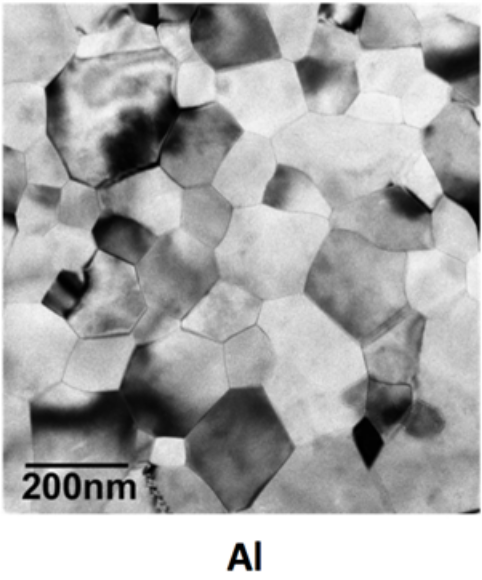
\includegraphics[scale=0.25, valign=t]{figures/extras/aluminum.png}\hspace{2em}
        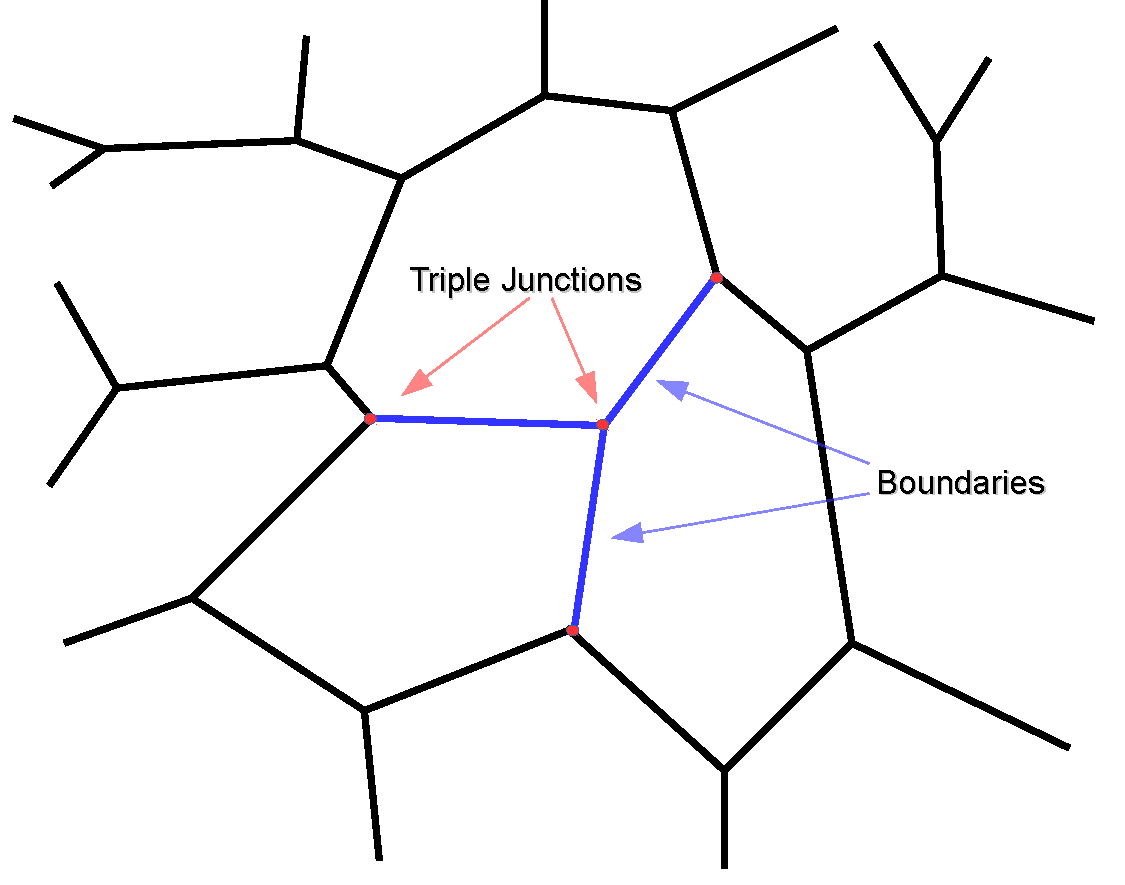
\includegraphics[scale=0.27,valign=t]{figures/extras/scheme.pdf}
    \end{figure}
    {\tiny \emph{Left: Aluminum thin film. Source: Internal communication between Dr. C. Torres and Dr. K. Barmak.}}
\end{frame}

\begin{frame}{Introduction}
    The orientation and shape of these grains define material's properties across wide scales such as thermal and electric conductivity, resistance, fracture toughness, corrosion resistance, among others~\cite{kinderlehrermultiscale, Kinderlehrer2006, Brons2013, torres2015}.

    \begin{figure}
        \centering
        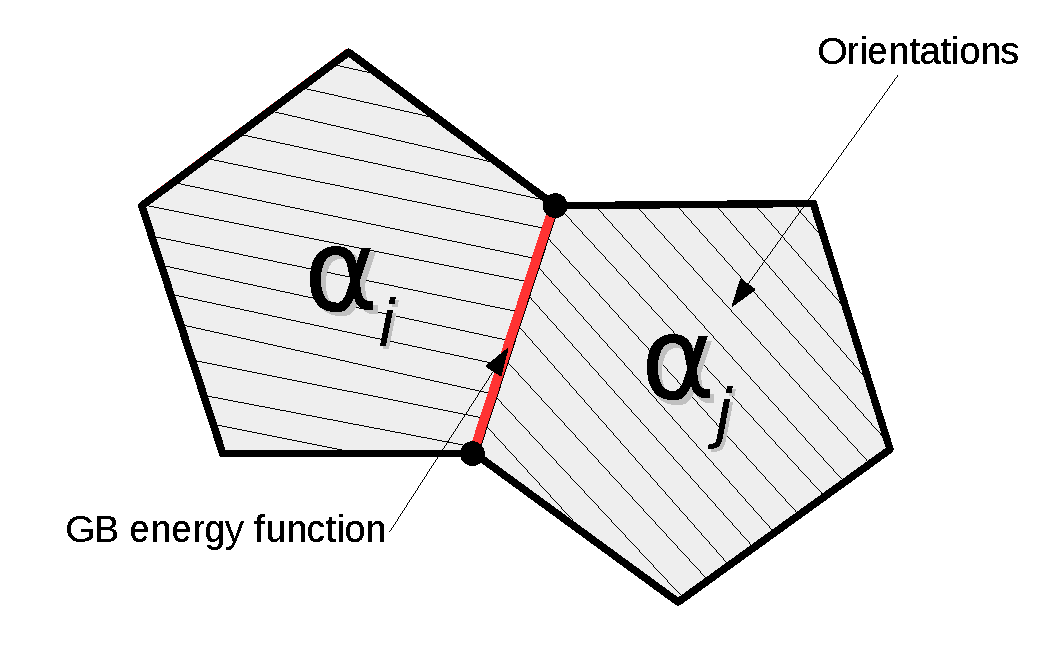
\includegraphics[scale=0.5]{figures/extras/grainenergy.pdf}
    \end{figure}
\end{frame}

\begin{frame}{Introduction}
    All of this allows the extraction of robust statistics that can be compared to the experimental data.  Computational scalability and performance of the implementation is important since running larger in short times is required to obtain more reliable statistics.\\

    This study has a strong emphasis on efficient implementation of the main presented models, specifically taking advantage of the graphic processing units (GPUs) [18, 17], allowing us to run simulations of the order of hundreds of thousands of grains.
\end{frame}

\begin{frame}{Objectives}
To contrast different grain growth mathematical models in 2D and 3D with the experimental data obtained from real materials through statistics related to geometry and energy of the grain structure. These statistics are average area, number of sides of each grain or grain class, dihedral angle at triple junctions, stored energy, grain boundary energy and misorientation.
\end{frame}

\begin{frame}{Objectives}
\begin{itemize}
    \item Analysis of curvature motion for boundaries and and stability study towards the improvement of the Coupled model developed in the bachelor thesis.
    \item Develop two-dimensional as well as three-dimensional models of grain growth and extract relevant statistics.
    \item Use a three-dimensional model of grain growth, generate two-dimensional slices and extract relevant statistics from them to analyze the relation with statistics from two-dimensional models.
\end{itemize}
\end{frame}


%%%% Big picture %%%%
% Define box and box title style
\section{Overview}

\tikzstyle{mybox} = [draw=blue, fill=blue!2, very thick, rectangle, rounded corners, inner sep=10pt, inner ysep=12pt]
\tikzstyle{fancytitle} =[draw=blue, fill=blue!6, very thick, text=black]
\tikzstyle{mybox2} = [draw=orange, fill=orange!2, very thick, rectangle, rounded corners, inner sep=10pt, inner ysep=12pt]
\tikzstyle{fancytitle2} =[draw=orange, fill=orange!6, very thick, text=black]

\begin{frame}
\centering
\begin{figure}[h]
\begin{tikzpicture}
\node [mybox, text width=0.9\textwidth] (box) {
\begin{minipage}[t]{0.46\textwidth}
\scriptsize
\textbf{The Coupled Model}

\vspace{0.5em}
\tiny
    Closed boundary study to capture curvature motion.\\

    Total Velocity as the result of a normal and tangential component.\\

    Multistep Euler and RK2, better estimation of $t_{\text{ext}}$.\\

    The Predictor-Corrector Algorithm.
\end{minipage}%
\hspace{2em}%
\begin{minipage}[t]{0.46\textwidth}
\scriptsize
\textbf{Stored Energy Vertex Model}

\vspace{0.5em}
\tiny
The Matrix-Free approach for estimating vertices velocities.\\

Effect of stored energy on the triple junctions dynamics.\\

How to nucleate, where, and which orientation we can use.
\end{minipage}\\
\vspace{1em}
\begin{minipage}[b]{1.1\textwidth}
\scriptsize
\textbf{The Parallel Polling System}

\vspace{0.5em}
\tiny
Both models are implemented in CUDA. Their topological transitions now are handled in parallel.
\end{minipage}
};
\node[fancytitle] at (box.north) {\small\textbf{2D Grain Growth}};
% %NOde for 3d
\node [mybox2, text width=0.9\textwidth] at ($(box.south)+(0,-2.1)$) (box2) {
\begin{minipage}[t]{0.46\textwidth}
\scriptsize
\textbf{The Implicit-transition Model}

\vspace{0.5em}
\tiny
Complex topological transitions handled.\\

We capture flippings, surface removals, grain removals.\\

Minimize energy asymptotically. Towards minimizing energy monotonically.
\end{minipage}%
\hspace{2em}%
\begin{minipage}[t]{0.46\textwidth}
\scriptsize
\textbf{Get 2D statistics from a 3D Code}

\vspace{0.5em}
\tiny
Perform simulations and store the cube of grains.\\

Get 2D slices and analyze them with image analysis software.
\end{minipage}
};
\node[fancytitle2] at (box2.north) {\small\textbf{3D Grain Growth}};
\end{tikzpicture}
\end{figure}
\end{frame}



%%% Coupled model %%%
\section{The Coupled Model}

\begin{frame}{Boundary Definition}
Consider the following boundary parametrization of $n$ collocation points:
\begin{equation*}
    \vxi(s,t) = \sum_{i=0}^n \x_i(t)\,\phi_i(s),\quad s \in [0, 1].
\end{equation*}
Where $\{\x_1,\x_n\}$ are triple junctions and $\{\x_2, \ldots, \x_{n-1}\}$ are interior points.
\vspace{-0.5em}
\begin{figure}
    \centering
    \begin{minipage}[t]{0.5\textwidth}
    \centering
    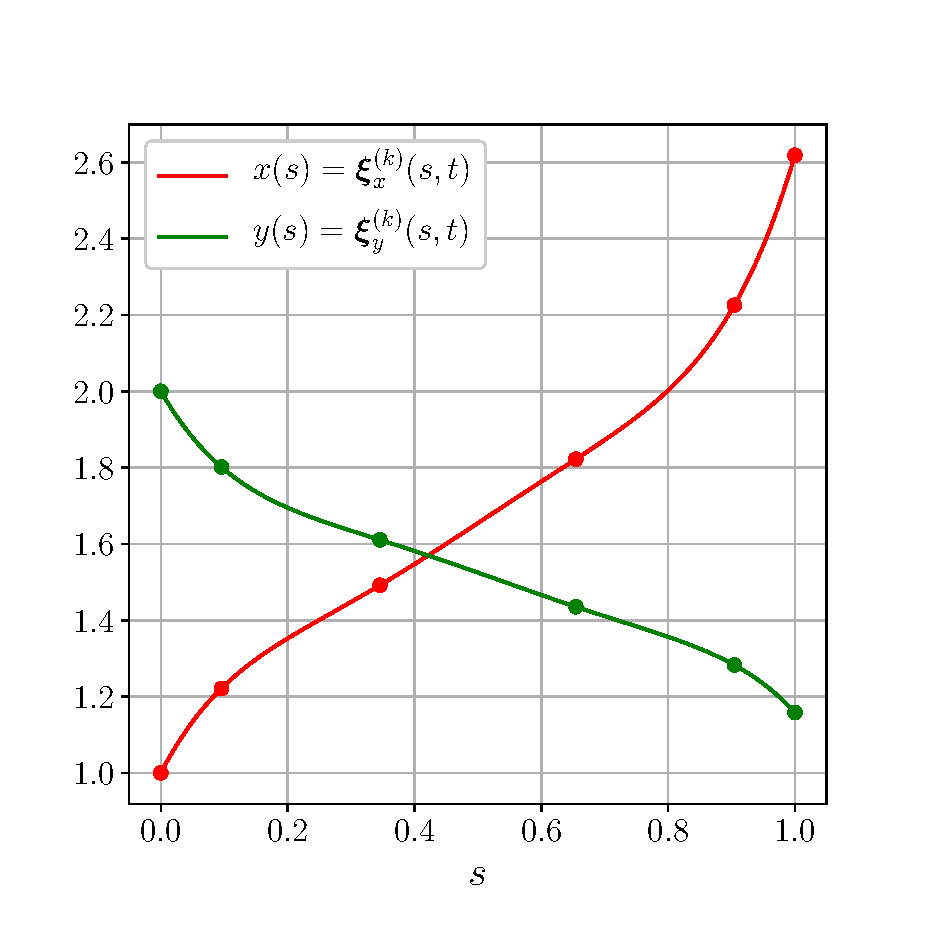
\includegraphics[scale=0.36,trim={0 0 0 3em},clip=true]{figures/coupled_model/xsys.eps}
    \end{minipage}%
    \begin{minipage}[t]{0.5\textwidth}
    \centering
    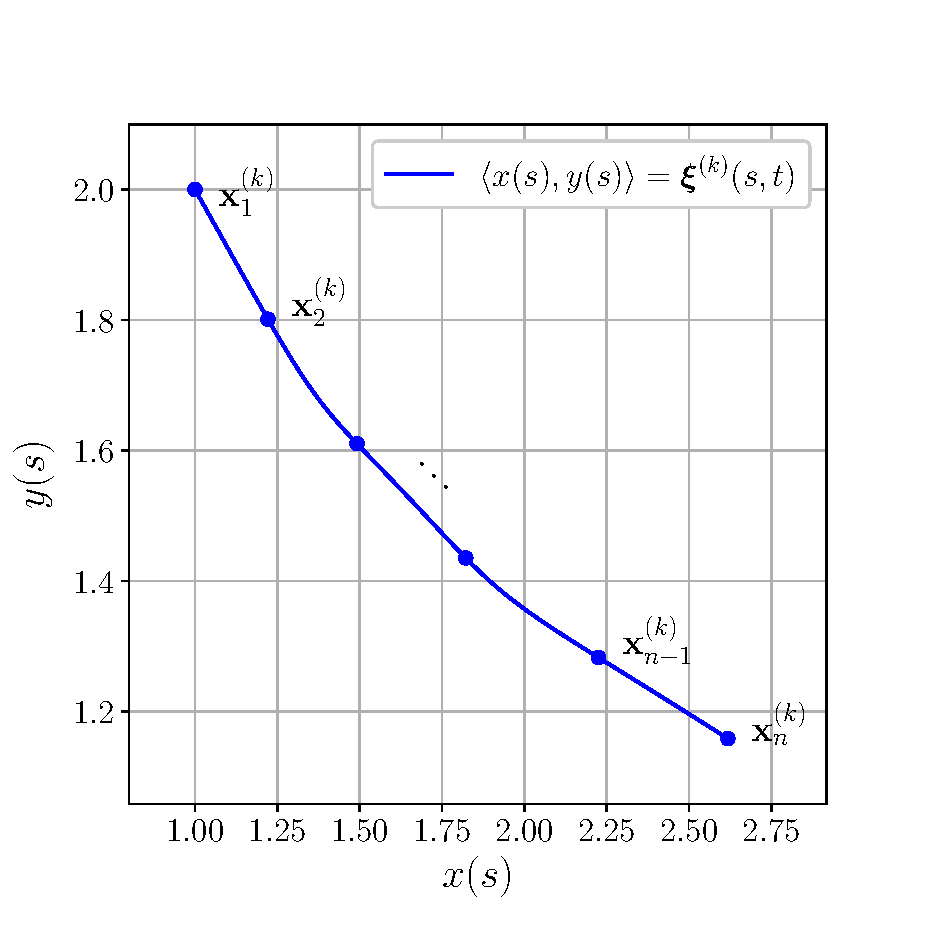
\includegraphics[scale=0.36,trim={0 0 0 3em},clip=true]{figures/coupled_model/xi.eps}
    \end{minipage}
\end{figure}
\end{frame}


\subsection{Model and Evolution Equations}

\begin{frame}{Model and Evolution Equations}
Recall the total energy of the system, given by:
\begin{equation*}
    E(t) = \sum_{k=1}^K \int_0^1 \gamma^{(k)} \norm{\mylvec^{(k)}(s,t)}\,ds,\quad \mylvec(s,t) = \frac{\partial \vxi}{\partial s}(s,t).
\end{equation*}
We evolve using a gradient descent algorithm, thus we compute $dE/dt$:
\vspace{-0.5em}
\small
\begin{multline}
    \frac{dE}{dt} =   -\sum_{k=1}^{K}\left[ \sum_{i=2}^{n-1} \dotx[i][k](t)  \cdot \int_0^1  \gamma^{(k)}\dTds^{(k)}\!\! \phi_i(s)\,ds \right] + \sum_{m=1}^{M} \vel_m(t) \cdot \sum_{l=1}^3 \gamma^{(m,l)}\T^{(m,l)}\\ -\sum_{m=1}^{M} \dotx[m]\,\,(t) \cdot \sum_{l=1}^3 \int_0^1 \gamma^{(m,l)} \dTds^{(m,l)}\phi_{1,m}(s)\,ds.  \label{eq:dEdtcoupled3}
    \end{multline}
\normalsize
The velocity of interior points $\dotx_i$ is defined as the sum of a normal and a tangential component. The normal component in principle is defined from $dE/dt$ as:
\begin{equation}
    \mathbf{N}^{(k)}_{i}(t) \approx \mu \gamma^{(k)}\!\int_0^1  \dTds^{(k)} (s,t) \phi_i(s)\,ds.
    \label{eq:incomplete_normalcomponent}
\end{equation}
\end{frame}

\begin{frame}{Evolution Equations}
\begin{minipage}[t]{0.5\textwidth}
The total velocity of interior points is defined as:
\begin{equation*}
\dotx_i(t) = \underbrace{\dotx_{i,\hatT}(t)}_{\displaystyle{\color{bb}\alpha_i(t) \hatT_i(t)}} + \underbrace{\dotx_{i,\hatN}(t)}_{\displaystyle {\color{red}\beta_i(t) \hatN_i(t)}}
\end{equation*}

\begin{itemize}
\item The {\color{red} normal} component, from Eq.~\eqref{eq:incomplete_normalcomponent}, aims to capture the curvature motion. It needs a correction for such task.

\item The {\color{bb} tangential} component helps to correct the interior points position along the boundary, avoiding coalescence.
\end{itemize}
\end{minipage}%
\begin{minipage}[t]{0.45\textwidth}
\centering
\begin{figure}
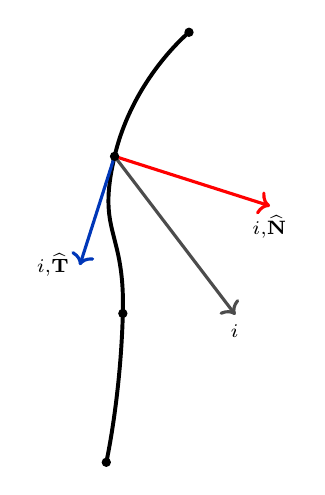
\begin{tikzpicture}[scale=1.05]
\coordinate (xini) at (0,0);
\coordinate (x1) at (0.2, 1.8);
\coordinate (x2) at (0.1, 3.7);
\coordinate (xend) at (1,5.2);
\coordinate (N) at (1.88, -0.6);
\coordinate (T) at (-0.7*0.6, -0.7*1.88);
\draw[line width=0.5mm] plot [smooth, tension=1] coordinates {(xini) (x1) (x2) (xend)};

\draw[->,Red,line width=0.4mm] (x2) -- ($(x2)+(N)$);
\draw[->,bb,line width=0.4mm] (x2) -- ($(x2)+(T)$);
\draw[->,black!70,line width=0.4mm] (x2) -- ($(x2)+(T)+(N)$);
\filldraw [black] (xini) circle (1.4pt);
\filldraw [black] (xend) circle (1.4pt);
\filldraw [black] (x1) circle (1.4pt);
\filldraw [black] (x2) circle (1.4pt);
\node[draw=none, color=black, below] at ($(x2)+(N)$) {$\dotx_{i,\hatN}$};
\node[draw=none, color=black, left] at ($(x2)+(T)$) {$\dotx_{i,\hatT}$};
\node[draw=none, color=black, below] at ($(x2)+(T)+(N)$) {$\dotx_{i}$};
\end{tikzpicture}
\end{figure}
\end{minipage}
\end{frame}

\begin{frame}{Improving the Normal Component}
    The normal component is improved from Eq.~\eqref{eq:incomplete_normalcomponent}.
    \begin{equation*}
         {\color{red}\beta_i(t)\hatN_i(t)} = \dotx_{i,\hatN}(t) = {\redbox}\,\mu\gamma \int_0^1 \dTds(s,t) \phi_i(s)\,ds.%,\quad i \in \{2,\ldots,n-1\}.
     \end{equation*}
    It just needs to be corrected by a factor \redbox\, that induces the curvature motion. Considering the curvature based velocity for a boundary~\cite{Kinderlehrer2006} we found that the missing term is $1/\norm{\mylvec(s,t)}$:
    \begin{equation*}
         {\color{red}\beta_i(t)\hatN_i(t)} = \dotx_{i,\hatN}(t) = \frac{\mu\gamma}{\color{red} \norm{\mylvec(s_i,t)}} \int_0^1 \dTds(s,t) \phi_i(s)\,ds.
     \end{equation*}
    This  correction still decreases the total energy $E(t)$.
    % The normal component is obtained from the previous definition of velocity:
    % \begin{equation*}
    %     {\color{red}\beta_i(t)\hatN_i(t)} = \dotx_{i,\hatN}(t) = {\redbox}\,\mu\gamma \int_0^1 \dTds(s,t) \phi_i(s)\,ds.%,\quad i \in \{2,\ldots,n-1\}.
    % \end{equation*}
    % It just needs to be corrected by a factor \redbox\, that induces the curvature motion. Consider the curvature based velocity for a boundary~\cite{Kinderlehrer2006} as:
    % \begin{equation*}
    %     \vel(s,t) = \kappa(s,t) \N(s,t)
    % \end{equation*}
    % Also, the derivative of the tangent vector to the boundary $\T$ with respect to the arc length yields:
    % \begin{equation*}
    %     \frac{\partial \T}{\partial \AL} = \frac{\partial \T}{\partial s} \frac{ds}{d\AL} = \kappa(s,t) \N(s,t)
    % \end{equation*}
\end{frame}


% \begin{frame}{Improving the Tangential Component}
%     The term $ds/d\AL$ is nothing but $1/\norm{\mylvec(s,t)}$, therefore:
%     \begin{equation*}
%         \vel(s,t) = \kappa(s,t) \N(s,t) = \frac{1}{\norm{\mylvec(s,t)}}\frac{\partial \T}{\partial s}(s,t).
%     \end{equation*}
%     Applying this equation to the  $\dotx_i(t)$ completes the missing \redbox\, term.
%     \begin{equation*}
%         {\color{red}\beta_i(t)\hatN_i(t)} = \dotx_{i,\hatN}(t) = \frac{\mu\gamma}{\color{red} \norm{\mylvec(s_i,t)}} \int_0^1 \dTds(s,t) \phi_i(s)\,ds.
%     \end{equation*}
% \end{frame}

\begin{frame}{Adding a Tangential Component}
    \begin{minipage}[t]{0.55\textwidth}
    Consider an initial equispaced distribution of points along the boundary. To keep them equispaced the following restriction has to be met~\cite{Mikula2001, Barrett2007, Barrett2010}:
    \begin{equation*}
        \dfrac{d}{dt}\left(\dfrac{\norm{\mylvec_i(t)}}{\AL(t)}\right)=0, \quad i\in \{2,\dots,n-2\},
    \end{equation*}
    where $\norm{\mylvec_i(t)}$ denotes the local arc length at collocation point $s_i$.

    This restriction is used to compute $\color{bb} \alpha_i(t)$ that will scale the unit tangent vector $\color{bb} \hatT_i$ orthogonal to the unit normal $\color{red}\hatN_i$.

    This introduced component also ensures decreasing the total energy.
    \end{minipage}%
    \begin{minipage}[t]{0.5\textwidth}
    \centering
\begin{figure}
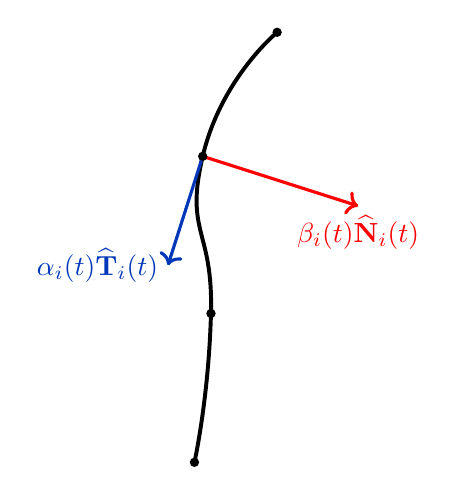
\begin{tikzpicture}[scale=1.05]
\coordinate (xini) at (0,0);
\coordinate (x1) at (0.2, 1.8);
\coordinate (x2) at (0.1, 3.7);
\coordinate (xend) at (1,5.2);
\coordinate (N) at (1.88, -0.6);
\coordinate (T) at (-0.7*0.6, -0.7*1.88);
\draw[line width=0.5mm] plot [smooth, tension=1] coordinates {(xini) (x1) (x2) (xend)};

\draw[->,Red,line width=0.4mm] (x2) -- ($(x2)+(N)$);
%\draw[->,bb,line width=0.4mm] (x2) -- ($(x2)+(T)$);
\draw[->,bb,line width=0.4mm] (x2) -- ($(x2)+(T)$);

%\draw[->,black!70,line width=0.4mm] (x2) -- ($(x2)+(T)+(N)$);
\filldraw [black] (xini) circle (1.4pt);
\filldraw [black] (xend) circle (1.4pt);
\filldraw [black] (x1) circle (1.4pt);
\filldraw [black] (x2) circle (1.4pt);
\node[draw=none, color=black, left] at ($(x2)+(T)$) {$\color{bb} \alpha_i(t)\hatT_i(t)$};
\node[draw=none, color=black, below] at ($(x2)+(N)$) {$\color{red} \beta_i(t)\hatN_i(t)$};

\end{tikzpicture}
\end{figure}
    \end{minipage}%
\end{frame}


\subsection{Flipping and Extinction Time Study}

\begin{frame}{Flipping and Extinction Time}
Topological transitions are the result of coarsening during grain growth.
\begin{itemize}
  \item Flippings
  \item Grain removals.
  \item Nucleations.
\end{itemize}
Flipping consists in the collapse of a boundary and switching neighboring boundaries, the new boundary then grows.
\begin{figure}
    \centering
    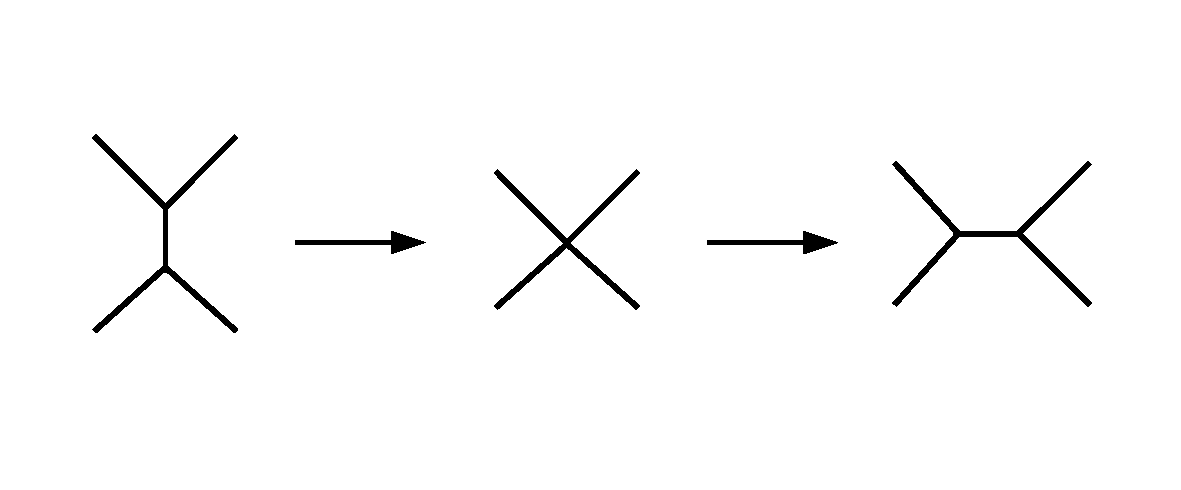
\includegraphics[scale=0.5]{figures/coupled_model/flipping.pdf}
\end{figure}
The time a boundary collapses is known as extinction time $t_\text{ext}$.
\end{frame}


\begin{frame}{Extinction Time Estimation and Flipping Detection}
$t_{\text{ext}}$ comes from a first order approximation and its error is proportional to $\Delta t$. We initially aim to detect flippings in $[0,\Delta t]$.
\begin{figure}
    \centering
    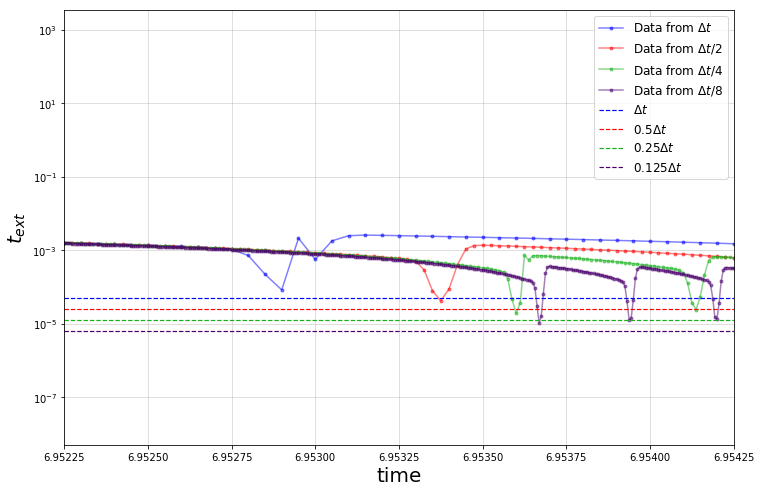
\includegraphics[scale=0.3]{figures/coupled_model/image_preview.png}
\end{figure}
Even if we reduce $\Delta t$ sometimes we will not be able to detect the flippings.
\end{frame}

\begin{frame}{Extinction Time Estimation and Flipping Detection}
    We developed \textbf{Multi-Step Algorithms} to improve $t_\text{ext}$ estimation.
    \begin{itemize}
        \item Euler Method of order $r$ and time step $\Delta \tau = \Delta t / r$
        \item Runge-Kutta 2. It can also be improved using $r$ multi steps.
    \end{itemize}
    \vspace{1em}
    We also improve the interval where we detect flippings as follows:

    \begin{figure}[t]
    \centering
    \begin{adjustbox}{max totalsize={.9\textwidth}{.7\textheight},center}
    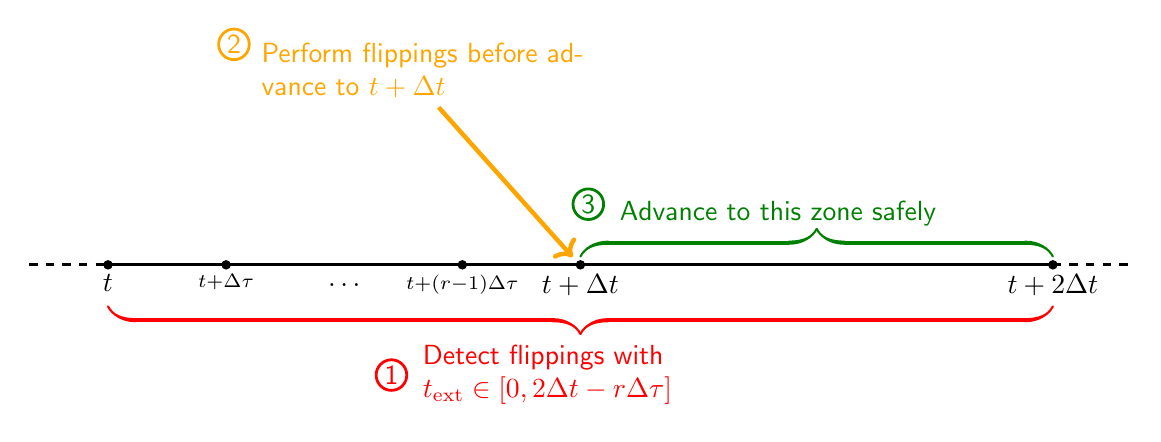
\begin{tikzpicture}
        % coordinates
        \coordinate (x0) at (-1,0);
        \coordinate (x1) at (0,0);
        \coordinate (x2) at (1.5,0);
        \coordinate (x3) at (3,0);
        \coordinate (x4) at (4.5,0);
        \coordinate (x5) at (6,0);
        \coordinate (x6) at (12,0);
        \coordinate (x7) at (13,0);
        \coordinate (A) at (4.2,2);

        % vertices
        \filldraw [black] (x1) circle (1.5pt);
        \filldraw [black] (x2) circle (1.5pt);
        %\filldraw [black] (x3) circle (1.5pt);
        \filldraw [black] (x4) circle (1.5pt);
        \filldraw [black] (x5) circle (1.5pt);
        \filldraw [black] (x6) circle (1.5pt);

        %%%%%%%%%%%%%%%%%%%%%%%%%%%%%%%%%%%%%%%%%%%%%
        % boundaries
        \draw[line width=0.4mm, black] (x1) -- (x6);
        \draw[line width=0.4mm, black, dashed] (x0) -- (x1);
        \draw[line width=0.4mm, black, dashed] (x6) -- (x7);

        \draw[decoration={calligraphic brace,mirror,amplitude=1em,raise=1.5em},decorate,line width=1.5pt, pen colour={Red}]
          (x1) -- node[below=2.5em, color=Red,text width=4cm] {\textsf{Detect flippings with} $t_{\text{ext}} \in [0, 2\Delta t- r\Delta \tau]$} (x6);

        \node[shape=circle,draw,inner sep=1pt,line width=1pt, color=Red] at (3.6,-1.4) {\textsf{1}};

        \node[shape=circle,draw,inner sep=1pt,line width=1pt, color=Green] at (6.1,0.77) {\textsf{3}};

        \draw[pen colour={Green}, decoration={calligraphic brace,amplitude=1em,raise=0.3em},decorate,line width=1.5pt]
          (x5) -- node[above=1em,color=Green,text width=5cm] {\textsf{Advance to this zone safely}} (x6);


         \node[shape=circle,draw,inner sep=1pt,line width=1pt, color=Orange] at (1.6,2.8) {\textsf{2}};

         \draw[->,Orange,ultra thick] (A) -- ($(x5)+(-0.1,0.1)$);
         \node[draw=none, color=Orange, above, text width=4.5cm] at (A) {\textsf{Perform flippings before advance to} $t+\Delta t$};

        % Text
        \node[draw=none, color=black, below] at (x1) {$t$};
        \node[draw=none, color=black, below] at (x2) {$\scriptstyle t+\Delta \tau$};
        \node[draw=none, color=black, below] at (x3) {$\phantom{a}\ldots\phantom{a}$};
        %{$\scriptstyle t+2\Delta \tau$};
        \node[draw=none, color=black, below] at (x4) {$\scriptstyle t+(r-1)\Delta \tau$};
        \node[draw=none, color=black, below] at (x5) {$t+\Delta  t$};
        \node[draw=none, color=black, below] at (x6) {$t+2\Delta  t$};
    \end{tikzpicture}
    \end{adjustbox}
    \end{figure}
\end{frame}


\begin{frame}{Curvature Near Collapse}
%When the boundaries are shrinking close to $t_\text{ext}$ the curvature of the boundary $\kappa(s)$ grows a lot and thus the vector $\beta_i\,\hatN_i$ is large, requiring a very small $\Delta t$ to perform a stable evolution.
Curvature grows as boundaries shrinks. This leads to large vectors $\beta_i\,\hatN_i$ and thus evolution requires very small $\Delta t$.
\vspace{-0.5em}
\begin{figure}
    \centering
    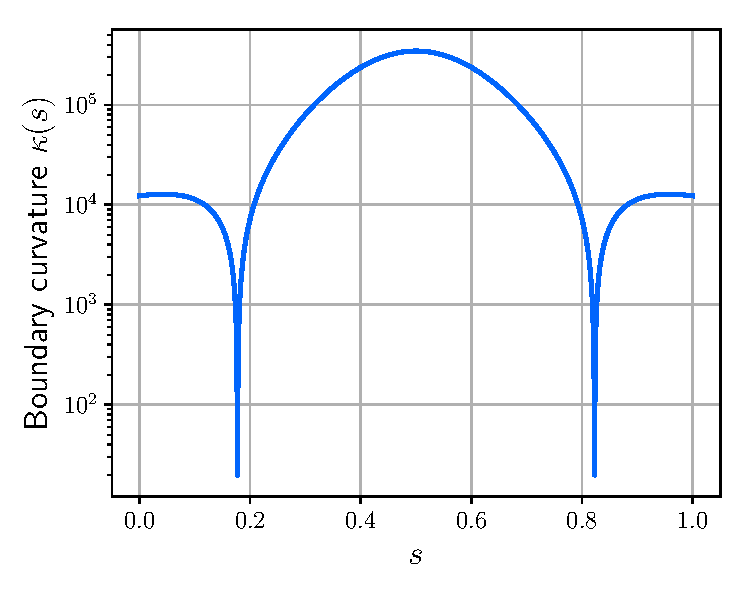
\includegraphics[scale=0.5]{figures/extras/curvature.pdf}
\end{figure}
\vspace{-1em}

Computing $\alpha_i\hatT_i$ depends on $\beta_i\,\hatN_i$ and thus also grows, which leads to unstable boundaries.%This leads to irregular boundary shapes and delayed flippings.

The \textbf{Predictor-Detector Algorithm} is used to overcome the growth.
%We must detect this behavior and prevent it by looking at the total velocity.
\end{frame}

\begin{frame}
    \begin{minipage}{0.45\textwidth}
    \small
    We begin by showing the interior points (\bluedot) and their \emph{candidate} steady state(\reddot) on the \emph{candidate} boundary steady state in dashed line.%. Notice that triple junctions have evolved to $t+\Delta t$.
    \end{minipage}\hspace{0.5em}%
    \begin{minipage}{0.53\textwidth}
    \begin{adjustbox}{max totalsize={\textwidth}{.7\textheight},center}
     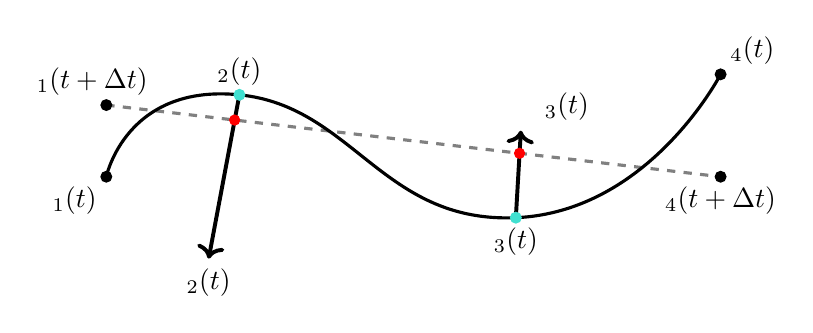
\begin{tikzpicture}[scale=1.3]
        % Vertices at time t
        \coordinate (x0) at (0,0);
        \coordinate (x1) at (6,1);
        % interior points at time t
        \coordinate (i0) at (1.3,0.8);
        \coordinate (i1) at (4,-0.4);
        % Vertices at time t+dt
        \coordinate (x2) at (0,0.7);
        \coordinate (x3) at (6,0);
        % interior points at time t+dt
        %\coordinate (i2) at (0.25, 4.5);
        %\coordinate (i3) at (4,-0.4);

        % Labels
        \node[draw=none, color=black, above left] at ($(x2) + (0.5,0)$) {$\x_1(t+\Delta t)$};
        \node[draw=none, color=black, below] at (x3) {$\x_4(t+\Delta t)$};
        \node[draw=none, color=black, below left] at (x0) {$\x_1(t)$};
        \node[draw=none, color=black, above right] at (x1) {$\x_4(t)$};
        \node[draw=none, color=black, above] at (i0) {$\x_2(t)$};
        \node[draw=none, color=black, below] at (i1) {$\x_3(t)$};

        \node[draw=none, color=black, below] at (1,-0.8) {$\dotx_2(t)$};
        \node[draw=none, color=black, above] at (4.5,0.45) {$\dotx_3(t)$};
        % Vertices have evolved and we mark de future steady state
         \draw[line width=0.4mm, black!50, dashed] (x2) -- (x3);
        % Draw the boundary as seen by the interior points which have not been moved
        \draw[line width=0.4mm] plot [smooth, tension=1] coordinates {(x0) (i0) (i1) (x1)};

        % Draw velocities
        \draw[->,black,line width=0.5mm] (i0) -- (1,-0.8);
        %\draw[->,black,line width=0.5mm] (i1) -- (4.1,1.3);
        \draw[->,black,line width=0.5mm] (i1) -- (4.05,0.45);

        % Draw vertices
        \filldraw [black] (x0) circle (1.5pt);
        \filldraw [black] (x1) circle (1.5pt);
        \filldraw [black] (x2) circle (1.5pt);
        \filldraw [black] (x3) circle (1.5pt);
        % Draw inner points
        \filldraw [Turquoise] (i0) circle (1.5pt);
        \filldraw [Turquoise] (i1) circle (1.5pt);
        %\filldraw [red] (i2) circle (1.5pt);
        %\filldraw [red] (i3) circle (1.5pt);
        \filldraw [red] (1.25382, 0.55372) circle (1.4pt);
        \filldraw [red] (4.037, 0.229015) circle (1.4pt);
    \end{tikzpicture}
    \end{adjustbox}
    \end{minipage}\\
    \textcolor{bb!50}{\rule{\textwidth}{0.1mm}}
    \begin{minipage}{0.45\textwidth}
    \small
    \textbf{Prediction}: Interior points predict their future positions (\bluedot) given the current velocities $\dotx_i(t)$.
    \end{minipage}\hspace{0.5em}%
    \begin{minipage}{0.53\textwidth}
      \begin{adjustbox}{max totalsize={\textwidth}{.7\textheight},center}
      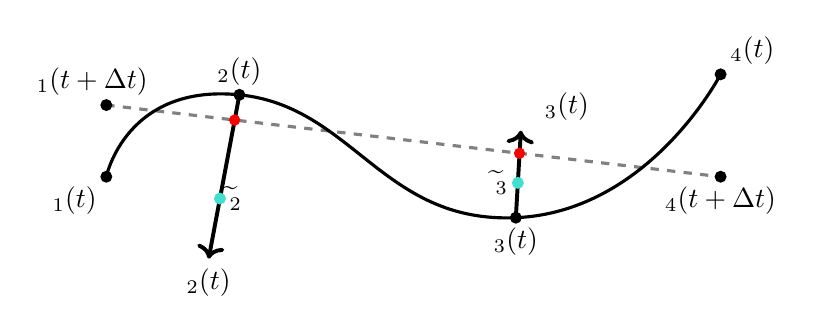
\begin{tikzpicture}[scale=1.3]
        % Vertices at time t
        \coordinate (x0) at (0,0);
        \coordinate (x1) at (6,1);
        % interior points at time t
        \coordinate (i0) at (1.3,0.8);
        \coordinate (i1) at (4,-0.4);
        % Vertices at time t+dt
        \coordinate (x2) at (0,0.7);
        \coordinate (x3) at (6,0);
        % interior points at time t+dt
        %\coordinate (i2) at (0.25, 4.5);
        %\coordinate (i3) at (4,-0.4);

        % Labels
        \node[draw=none, color=black, above left] at ($(x2) + (0.5,0)$) {$\x_1(t+\Delta t)$};
        \node[draw=none, color=black, below] at (x3) {$\x_4(t+\Delta t)$};
        \node[draw=none, color=black, below left] at (x0) {$\x_1(t)$};
        \node[draw=none, color=black, above right] at (x1) {$\x_4(t)$};
        \node[draw=none, color=black, above] at (i0) {$\x_2(t)$};
        \node[draw=none, color=black, below] at (i1) {$\x_3(t)$};

        \node[draw=none, color=black, below] at (1,-0.8) {$\dotx_2(t)$};
        \node[draw=none, color=black, above] at (4.5,0.45) {$\dotx_3(t)$};
        % Vertices have evolved and we mark de future steady state
         \draw[line width=0.4mm, black!50, dashed] (x2) -- (x3);
        % Draw the boundary as seen by the interior points which have not been moved
        \draw[line width=0.4mm] plot [smooth, tension=1] coordinates {(x0) (i0) (i1) (x1)};

        % Draw velocities
        \draw[->,black,line width=0.5mm] (i0) -- (1,-0.8);
        %\draw[->,black,line width=0.5mm] (i1) -- (4.1,1.3);
        \draw[->,black,line width=0.5mm] (i1) -- (4.05,0.45);

        % Draw vertices
        \filldraw [black] (x0) circle (1.5pt);
        \filldraw [black] (x1) circle (1.5pt);
        \filldraw [black] (x2) circle (1.5pt);
        \filldraw [black] (x3) circle (1.5pt);
        % Draw inner points
        \filldraw [black] (i0) circle (1.5pt);
        \filldraw [black] (i1) circle (1.5pt);

        \coordinate (pred1) at (1.11, -0.213333);
        \coordinate (pred2) at (4.02,-0.06);
        % Draw predictions
        \filldraw [Turquoise] (pred1) circle (1.5pt);
        \filldraw [Turquoise] (pred2) circle (1.5pt);

        \node[draw=none, color=black, right] at (pred1) {$\widetilde{\x}_2$};
        \node[draw=none, color=black, left] at (pred2) {$\widetilde{\x}_3$};

        \filldraw [red] (1.25382, 0.55372) circle (1.4pt);
        \filldraw [red] (4.037, 0.229015) circle (1.4pt);
    \end{tikzpicture}
    \end{adjustbox}
    \end{minipage}\\
    \textcolor{bb!50}{\rule{\textwidth}{0.1mm}}
    \begin{minipage}{0.45\textwidth}
    \small
    Velocities are recomputed such that interior points position at $t+\Delta t$ (\bluedot) is at most the \emph{candidate} steady state.
    \end{minipage}\hspace{0.5em}%
    \begin{minipage}{0.53\textwidth}
    \begin{adjustbox}{max totalsize={\textwidth}{.7\textheight},center}
       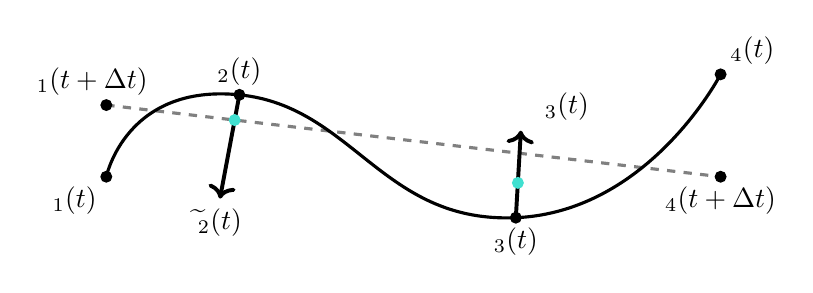
\begin{tikzpicture}[scale=1.3]
        % Vertices at time t
        \coordinate (x0) at (0,0);
        \coordinate (x1) at (6,1);
        % interior points at time t
        \coordinate (i0) at (1.3,0.8);
        \coordinate (i1) at (4,-0.4);
        % Vertices at time t+dt
        \coordinate (x2) at (0,0.7);
        \coordinate (x3) at (6,0);
        \coordinate (pred1) at (1.25382, 0.55372);
        \coordinate (pred2) at (4.02,-0.06);
        % Labels
        \node[draw=none, color=black, above left] at ($(x2)+(0.5,0)$) {$\x_1(t+\Delta t)$};
        \node[draw=none, color=black, below] at (x3) {$\x_4(t+\Delta t)$};
        \node[draw=none, color=black, below left] at (x0) {$\x_1(t)$};
        \node[draw=none, color=black, above right] at (x1) {$\x_4(t)$};
        \node[draw=none, color=black, above] at (i0) {$\x_2(t)$};
        \node[draw=none, color=black, below] at (i1) {$\x_3(t)$};

        \coordinate (endvel) at (1.11, -0.21333);
        \node[draw=none, color=black, below] at (endvel) {$\widetilde{\dotx}_2(t)$};
        \node[draw=none, color=black, above] at (4.5,0.45) {$\dotx_3(t)$};

        % Vertices have evolved and we mark de future steady state
         \draw[line width=0.4mm, black!50, dashed] (x2) -- (x3);
        % Draw the boundary as seen by the interior points which have not been moved
        \draw[line width=0.4mm] plot [smooth, tension=1] coordinates {(x0) (i0) (i1) (x1)};

        % Draw velocities
        %\draw[->,black,line width=0.5mm] (i0) -- (1,-0.8);
        \draw[->,black,line width=0.5mm] (i0) -- (endvel);
        \draw[->,black,line width=0.5mm] (i1) -- (4.05,0.45);

        % Draw vertices
        \filldraw [black] (x0) circle (1.5pt);
        \filldraw [black] (x1) circle (1.5pt);
        \filldraw [black] (x2) circle (1.5pt);
        \filldraw [black] (x3) circle (1.5pt);
        % Draw inner points
        \filldraw [black] (i0) circle (1.5pt);
        \filldraw [black] (i1) circle (1.5pt);


        % Draw predictions
        \filldraw [Turquoise] (pred1) circle (1.5pt);
        \filldraw [Turquoise] (pred2) circle (1.5pt);
    \end{tikzpicture}
    \end{adjustbox}
    \end{minipage}\\
    \textcolor{bb!50}{\rule{\textwidth}{0.1mm}}
    \begin{minipage}{0.45\textwidth}
     \vspace{1em}
    \small
    %The \textbf{correction} stage: The interior points are moved with the corrected velocities. Now the boundary has evolved completely to $t+\Delta t$.
    \textbf{Correction}: Interior points are moved with the corrected velocities. Now the boundary has evolved completely to $t+\Delta t$.
    \end{minipage}\hspace{0.5em}%
    \begin{minipage}{0.53\textwidth}
    \begin{adjustbox}{max totalsize={\textwidth}{.7\textheight},center}
    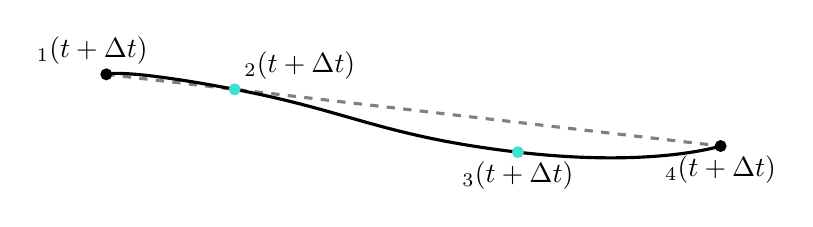
\begin{tikzpicture}[scale=1.3]
        % Vertices at time t
        %\coordinate (x0) at (0,0);
        %\coordinate (x1) at (6,1);
        % Vertices at time t+dt
        \coordinate (x2) at (0,0.7);
        \coordinate (x3) at (6,0);

        \coordinate (pred1) at (1.25382, 0.55372);
        \coordinate (pred2) at (4.02,-0.06);


        % Labels
        \node[draw=none, color=black, above left] at ($(x2)+(0.5,0)$) {$\x_1(t+\Delta t)$};
        \node[draw=none, color=black, below] at (x3) {$\x_4(t+\Delta t)$};
        %\node[draw=none, color=black, below left] at (x0) {$\x_1(t)$};
        %\node[draw=none, color=black, above right] at (x1) {$\x_4(t)$};
        \node[draw=none, color=black, above right] at (pred1) {$\x_2(t+\Delta t)$};
        \node[draw=none, color=black, below] at (pred2) {$\x_3(t+\Delta t)$};

        % Vertices have evolved and we mark de future steady state
         \draw[line width=0.4mm, black!50, dashed] (x2) -- (x3);
        % Draw the boundary as seen by the interior points which have not been moved
        \draw[line width=0.4mm] plot [smooth, tension=1] coordinates {(x2) (pred1) (pred2) (x3)};

        % Draw vertices
        \filldraw [black] (x2) circle (1.5pt);
        \filldraw [black] (x3) circle (1.5pt);

        % Draw predictions
        \filldraw [Turquoise] (pred1) circle (1.5pt);
        \filldraw [Turquoise] (pred2) circle (1.5pt);
    \end{tikzpicture}
    \end{adjustbox}
    \end{minipage}
\end{frame}

% \begin{frame}{The Predictor-Corrector Algorithm}
%  \begin{tikzpicture}[scale=1.3]
%         % Vertices at time t
%         \coordinate (x0) at (0,0);
%         \coordinate (x1) at (6,1);
%         % interior points at time t
%         \coordinate (i0) at (1.3,0.8);
%         \coordinate (i1) at (4,-0.4);
%         % Vertices at time t+dt
%         \coordinate (x2) at (0,0.7);
%         \coordinate (x3) at (6,0);
%         % interior points at time t+dt
%         %\coordinate (i2) at (0.25, 4.5);
%         %\coordinate (i3) at (4,-0.4);

%         % Labels
%         \node[draw=none, color=black, above left] at (x2) {$\x_1(t+\Delta t)$};
%         \node[draw=none, color=black, below right] at (x3) {$\x_4(t+\Delta t)$};
%         \node[draw=none, color=black, below left] at (x0) {$\x_1(t)$};
%         \node[draw=none, color=black, above right] at (x1) {$\x_4(t)$};
%         \node[draw=none, color=black, above] at (i0) {$\x_2(t)$};
%         \node[draw=none, color=black, below] at (i1) {$\x_3(t)$};

%         \node[draw=none, color=black, below] at (1,-0.8) {$\dotx_2(t)$};
%         \node[draw=none, color=black, above] at (4.5,0.45) {$\dotx_3(t)$};
%         % Vertices have evolved and we mark de future steady state
%          \draw[line width=0.4mm, black!50, dashed] (x2) -- (x3);
%         % Draw the boundary as seen by the interior points which have not been moved
%         \draw[line width=0.4mm] plot [smooth, tension=1] coordinates {(x0) (i0) (i1) (x1)};

%         % Draw velocities
%         \draw[->,black,line width=0.5mm] (i0) -- (1,-0.8);
%         %\draw[->,black,line width=0.5mm] (i1) -- (4.1,1.3);
%         \draw[->,black,line width=0.5mm] (i1) -- (4.05,0.45);

%         % Draw vertices
%         \filldraw [black] (x0) circle (1.5pt);
%         \filldraw [black] (x1) circle (1.5pt);
%         \filldraw [black] (x2) circle (1.5pt);
%         \filldraw [black] (x3) circle (1.5pt);
%         % Draw inner points
%         \filldraw [Turquoise] (i0) circle (1.5pt);
%         \filldraw [Turquoise] (i1) circle (1.5pt);
%         %\filldraw [red] (i2) circle (1.5pt);
%         %\filldraw [red] (i3) circle (1.5pt);
%         \filldraw [red] (1.25382, 0.55372) circle (1.4pt);
%         \filldraw [red] (4.037, 0.229015) circle (1.4pt);
%     \end{tikzpicture}
% We begin by showing the interior points (\bluedot) and the \emph{candidate} steady state for each one (\reddot) on the \emph{candidate} boundary steady state (\bndsteady). Notice that triple junctions have evolved to $t+\Delta t$.
% \end{frame}

% \begin{frame}{The Predictor-Corrector Algorithm}
%     \begin{tikzpicture}[scale=1.3]
%         % Vertices at time t
%         \coordinate (x0) at (0,0);
%         \coordinate (x1) at (6,1);
%         % interior points at time t
%         \coordinate (i0) at (1.3,0.8);
%         \coordinate (i1) at (4,-0.4);
%         % Vertices at time t+dt
%         \coordinate (x2) at (0,0.7);
%         \coordinate (x3) at (6,0);
%         % interior points at time t+dt
%         %\coordinate (i2) at (0.25, 4.5);
%         %\coordinate (i3) at (4,-0.4);

%         % Labels
%         \node[draw=none, color=black, above left] at (x2) {$\x_1(t+\Delta t)$};
%         \node[draw=none, color=black, below right] at (x3) {$\x_4(t+\Delta t)$};
%         \node[draw=none, color=black, below left] at (x0) {$\x_1(t)$};
%         \node[draw=none, color=black, above right] at (x1) {$\x_4(t)$};
%         \node[draw=none, color=black, above] at (i0) {$\x_2(t)$};
%         \node[draw=none, color=black, below] at (i1) {$\x_3(t)$};

%         \node[draw=none, color=black, below] at (1,-0.8) {$\dotx_2(t)$};
%         \node[draw=none, color=black, above] at (4.5,0.45) {$\dotx_3(t)$};
%         % Vertices have evolved and we mark de future steady state
%          \draw[line width=0.4mm, black!50, dashed] (x2) -- (x3);
%         % Draw the boundary as seen by the interior points which have not been moved
%         \draw[line width=0.4mm] plot [smooth, tension=1] coordinates {(x0) (i0) (i1) (x1)};

%         % Draw velocities
%         \draw[->,black,line width=0.5mm] (i0) -- (1,-0.8);
%         %\draw[->,black,line width=0.5mm] (i1) -- (4.1,1.3);
%         \draw[->,black,line width=0.5mm] (i1) -- (4.05,0.45);

%         % Draw vertices
%         \filldraw [black] (x0) circle (1.5pt);
%         \filldraw [black] (x1) circle (1.5pt);
%         \filldraw [black] (x2) circle (1.5pt);
%         \filldraw [black] (x3) circle (1.5pt);
%         % Draw inner points
%         \filldraw [black] (i0) circle (1.5pt);
%         \filldraw [black] (i1) circle (1.5pt);

%         \coordinate (pred1) at (1.11, -0.213333);
%         \coordinate (pred2) at (4.02,-0.06);
%         % Draw predictions
%         \filldraw [Turquoise] (pred1) circle (1.5pt);
%         \filldraw [Turquoise] (pred2) circle (1.5pt);

%         \node[draw=none, color=black, right] at (pred1) {$\widetilde{\x}_2$};
%         \node[draw=none, color=black, left] at (pred2) {$\widetilde{\x}_3$};

%         \filldraw [red] (1.25382, 0.55372) circle (1.4pt);
%         \filldraw [red] (4.037, 0.229015) circle (1.4pt);
%     \end{tikzpicture}
% The \textbf{prediction} stage: The interior points predict their future positions (\bluedot) given the current velocities $\dotx_i(t)$.
% \end{frame}

% \begin{frame}{The Predictor-Corrector Algorithm}
%      \begin{tikzpicture}[scale=1.3]
%         % Vertices at time t
%         \coordinate (x0) at (0,0);
%         \coordinate (x1) at (6,1);
%         % interior points at time t
%         \coordinate (i0) at (1.3,0.8);
%         \coordinate (i1) at (4,-0.4);
%         % Vertices at time t+dt
%         \coordinate (x2) at (0,0.7);
%         \coordinate (x3) at (6,0);
%         \coordinate (pred1) at (1.25382, 0.55372);
%         \coordinate (pred2) at (4.02,-0.06);
%         % Labels
%         \node[draw=none, color=black, above left] at (x2) {$\x_1(t+\Delta t)$};
%         \node[draw=none, color=black, below right] at (x3) {$\x_4(t+\Delta t)$};
%         \node[draw=none, color=black, below left] at (x0) {$\x_1(t)$};
%         \node[draw=none, color=black, above right] at (x1) {$\x_4(t)$};
%         \node[draw=none, color=black, above] at (i0) {$\x_2(t)$};
%         \node[draw=none, color=black, below] at (i1) {$\x_3(t)$};

%         \coordinate (endvel) at (1.11, -0.21333);
%         \node[draw=none, color=black, below] at (endvel) {$\widetilde{\dotx}_2(t)$};
%         \node[draw=none, color=black, above] at (4.5,0.45) {$\dotx_3(t)$};

%         % Vertices have evolved and we mark de future steady state
%          \draw[line width=0.4mm, black!50, dashed] (x2) -- (x3);
%         % Draw the boundary as seen by the interior points which have not been moved
%         \draw[line width=0.4mm] plot [smooth, tension=1] coordinates {(x0) (i0) (i1) (x1)};

%         % Draw velocities
%         %\draw[->,black,line width=0.5mm] (i0) -- (1,-0.8);
%         \draw[->,black,line width=0.5mm] (i0) -- (endvel);
%         \draw[->,black,line width=0.5mm] (i1) -- (4.05,0.45);

%         % Draw vertices
%         \filldraw [black] (x0) circle (1.5pt);
%         \filldraw [black] (x1) circle (1.5pt);
%         \filldraw [black] (x2) circle (1.5pt);
%         \filldraw [black] (x3) circle (1.5pt);
%         % Draw inner points
%         \filldraw [black] (i0) circle (1.5pt);
%         \filldraw [black] (i1) circle (1.5pt);


%         % Draw predictions
%         \filldraw [Turquoise] (pred1) circle (1.5pt);
%         \filldraw [Turquoise] (pred2) circle (1.5pt);
%     \end{tikzpicture}

% \vspace{1em}
% Velocities are recomputed such that the interior points position at $t+\Delta t$ (\bluedot) is at most the \emph{candidate} steady state.
% \end{frame}

% \begin{frame}{}
%     \begin{tikzpicture}[scale=1.3]
%         % Vertices at time t
%         %\coordinate (x0) at (0,0);
%         %\coordinate (x1) at (6,1);
%         % Vertices at time t+dt
%         \coordinate (x2) at (0,0.7);
%         \coordinate (x3) at (6,0);

%         \coordinate (pred1) at (1.25382, 0.55372);
%         \coordinate (pred2) at (4.02,-0.06);


%         % Labels
%         \node[draw=none, color=black, above left] at (x2) {$\x_1(t+\Delta t)$};
%         \node[draw=none, color=black, below right] at (x3) {$\x_4(t+\Delta t)$};
%         %\node[draw=none, color=black, below left] at (x0) {$\x_1(t)$};
%         %\node[draw=none, color=black, above right] at (x1) {$\x_4(t)$};
%         \node[draw=none, color=black, above right] at (pred1) {$\x_2(t+\Delta t)$};
%         \node[draw=none, color=black, below] at (pred2) {$\x_3(t+\Delta t)$};

%         % Vertices have evolved and we mark de future steady state
%          \draw[line width=0.4mm, black!50, dashed] (x2) -- (x3);
%         % Draw the boundary as seen by the interior points which have not been moved
%         \draw[line width=0.4mm] plot [smooth, tension=1] coordinates {(x2) (pred1) (pred2) (x3)};

%         % Draw vertices
%         %\filldraw [black] (x0) circle (1.5pt);
%         %\filldraw [black] (x1) circle (1.5pt);
%         \filldraw [black] (x2) circle (1.5pt);
%         \filldraw [black] (x3) circle (1.5pt);

%         % Draw predictions
%         \filldraw [Turquoise] (pred1) circle (1.5pt);
%         \filldraw [Turquoise] (pred2) circle (1.5pt);
%     \end{tikzpicture}

% \vspace{2em}
% The \textbf{correction} stage: The interior points are moved with the corrected velocities. Now the boundary has evolved completely to $t+\Delta t$.
% \end{frame}

\subsection{Numerical Experiments}

\begin{frame}{Numerical Experiments}
   \centering
   \movie[width=\textwidth,height=\textheight]{Simulation}{/home/asazo/Escritorio/coupled.mov}
\end{frame}

\begin{frame}{Numerical Experiments}
\begin{figure}
    %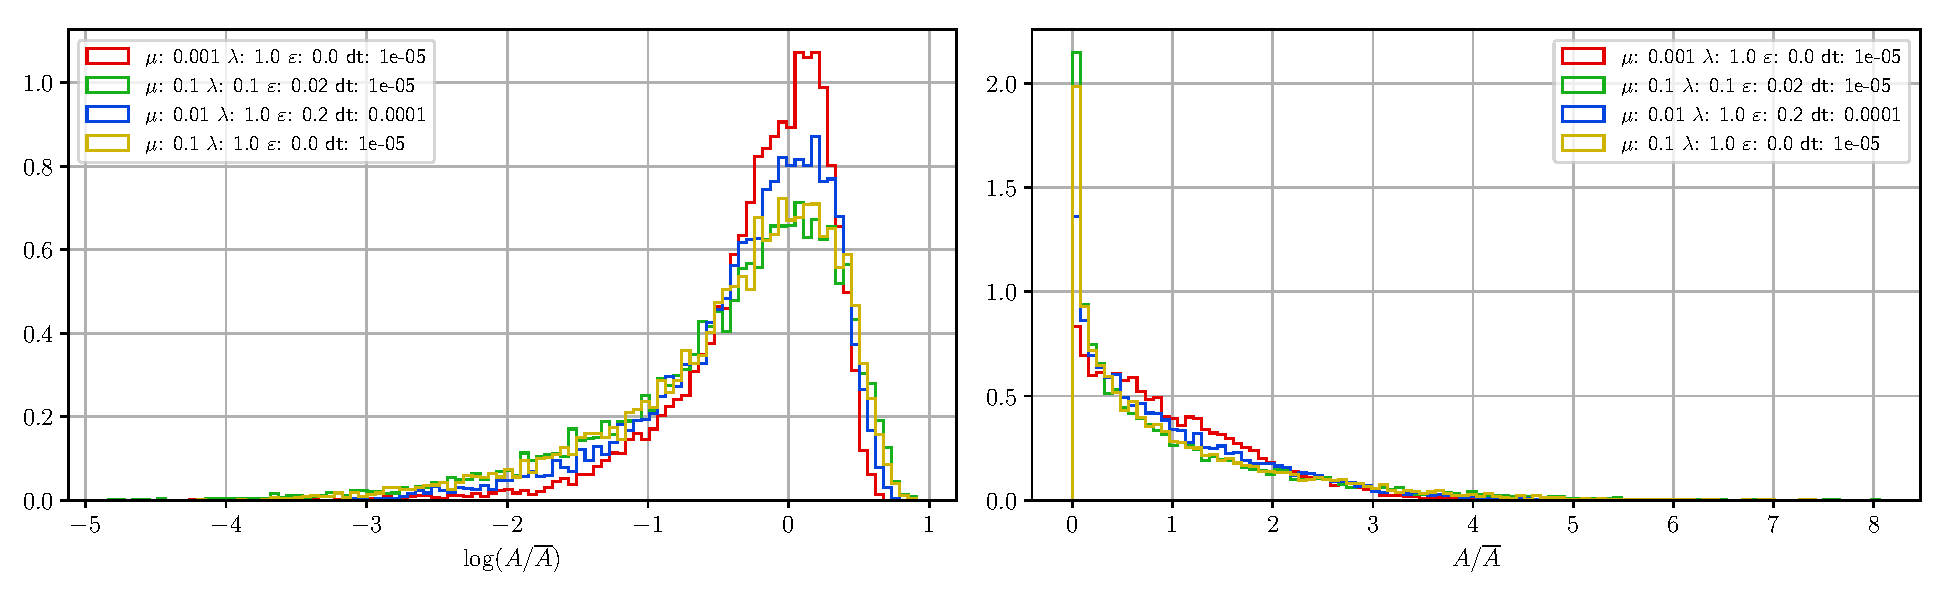
\includegraphics[trim={0 0 44em 0},clip=true,scale=0.4]{figures/coupled_model/new_data/areas.pdf}
    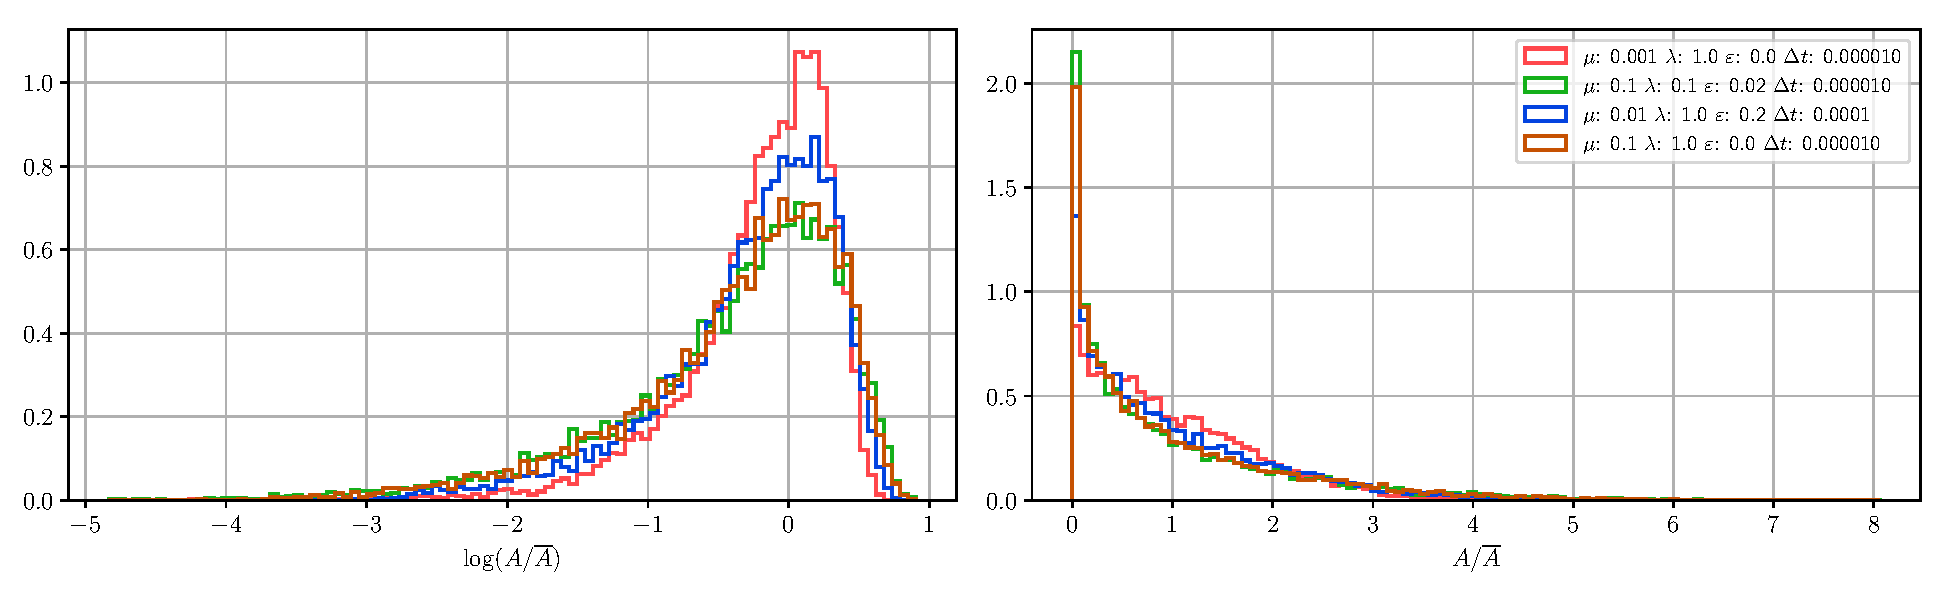
\includegraphics[trim={0 0 44em 0},clip=true,scale=0.4]{figures/coupled_model/alt/areas.pdf}
\end{figure}
\vspace{-1.5em}
\begin{figure}
    %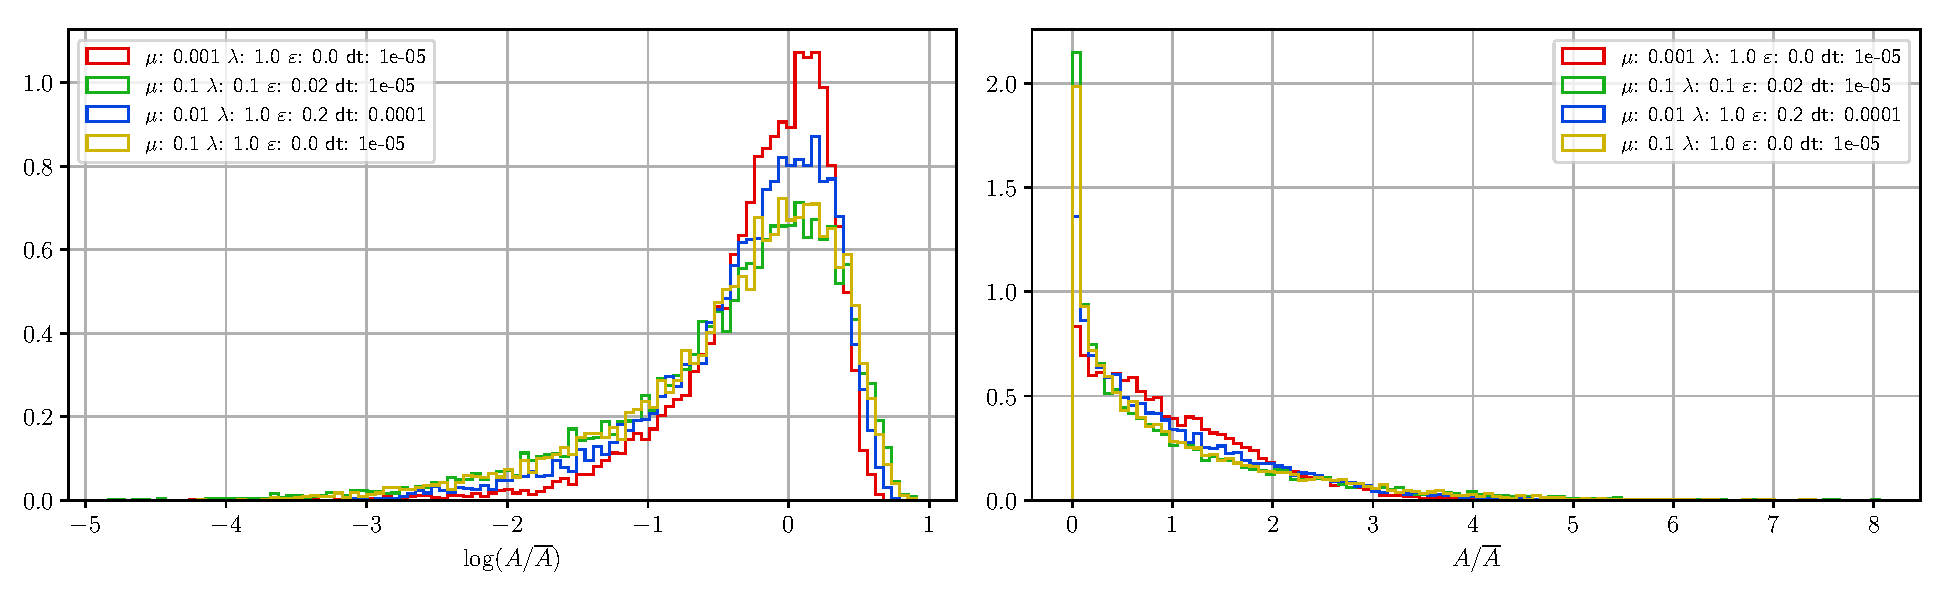
\includegraphics[trim={43em 0 0 0},clip=true,scale=0.4]{figures/coupled_model/new_data/areas.pdf}
    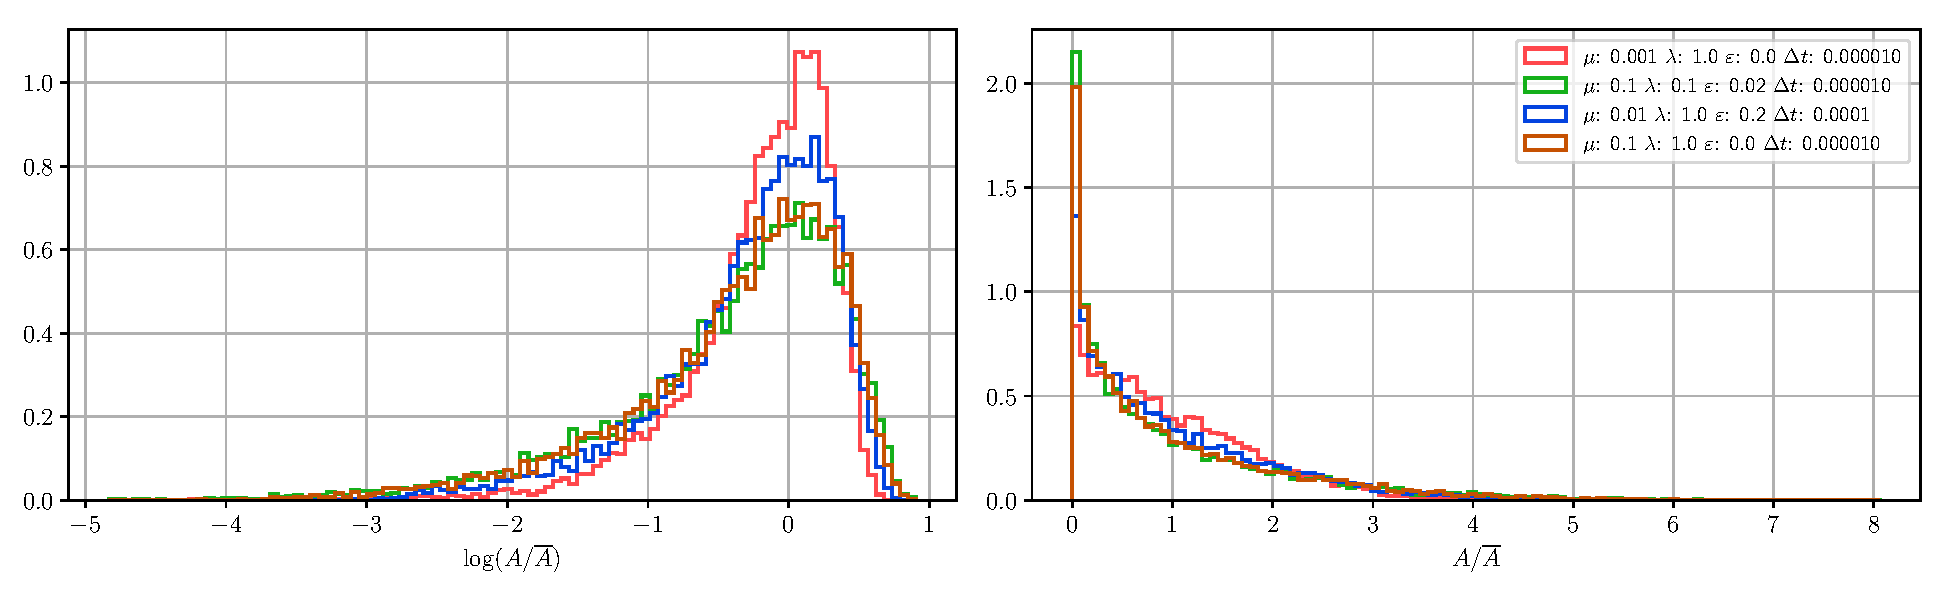
\includegraphics[trim={43em 0 0 0},clip=true,scale=0.4]{figures/coupled_model/alt/areas.pdf}
\end{figure}
\end{frame}

\begin{frame}{Numerical Experiments}
\vspace{-0.5em}
\begin{minipage}{0.5\textwidth}
\begin{figure}
    %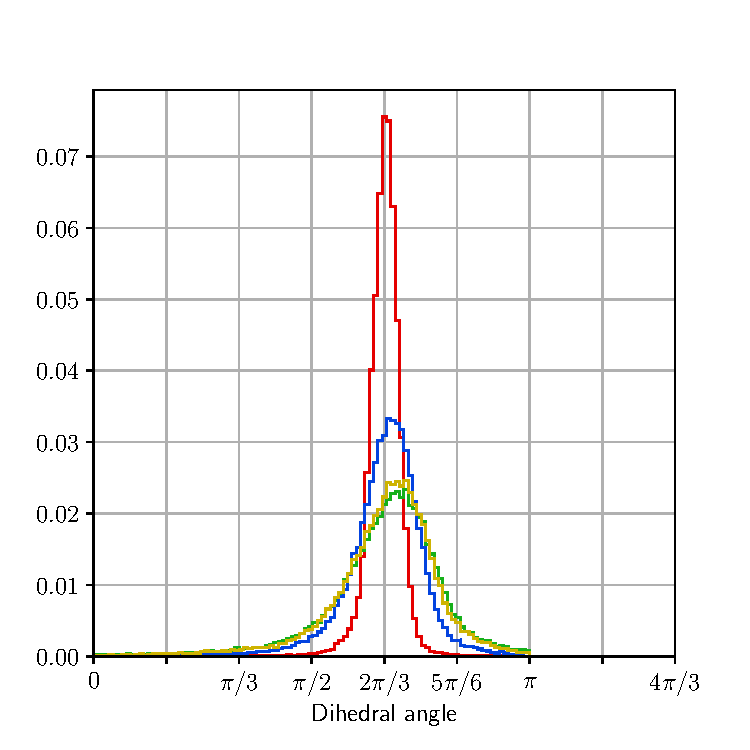
\includegraphics[trim={0 1em 0 3em},clip=true,scale=0.35]{figures/coupled_model/new_data/ang.pdf}
    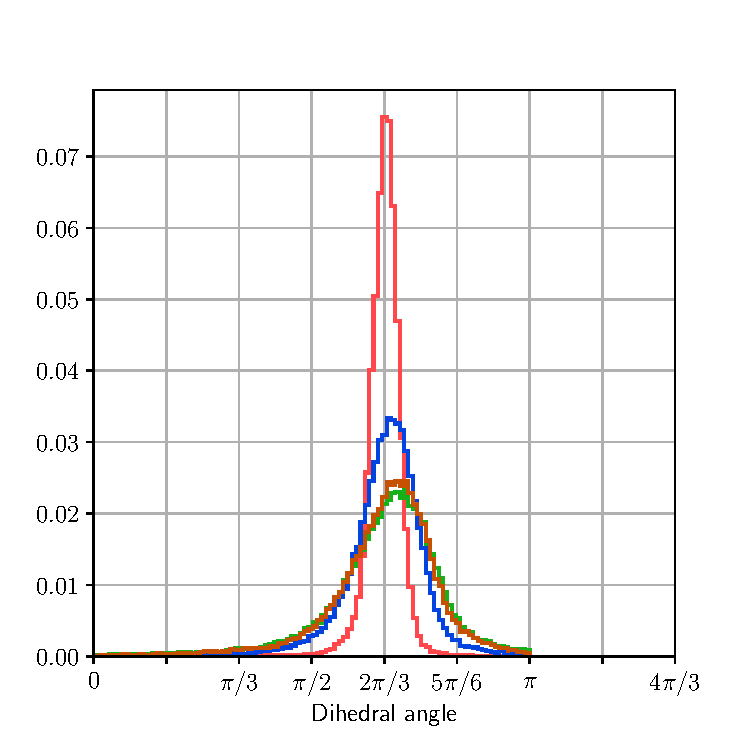
\includegraphics[trim={0 1em 0 3em},clip=true,scale=0.35]{figures/coupled_model/alt/ang.pdf}
\end{figure}
\end{minipage}%
\begin{minipage}{0.5\textwidth}
\begin{figure}
   %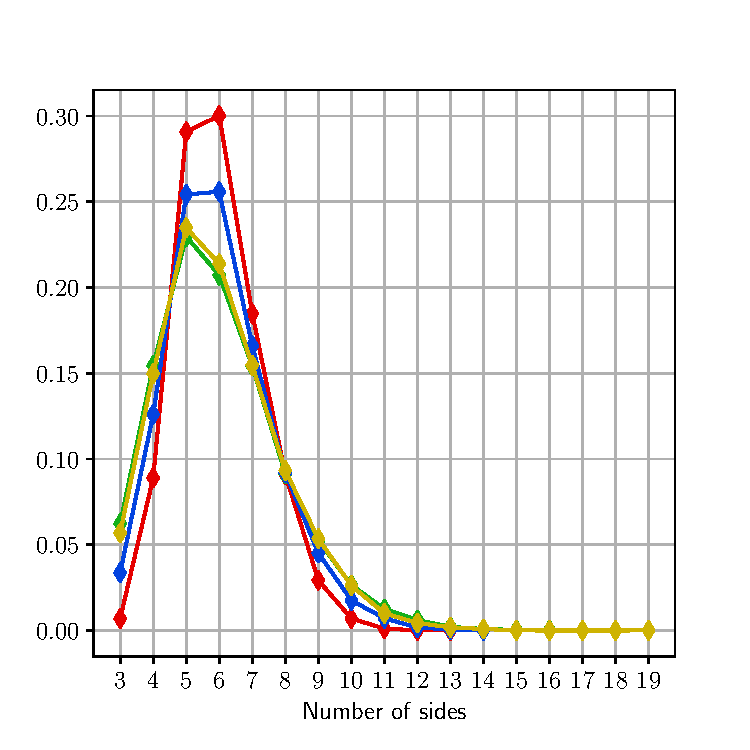
\includegraphics[trim={0 1em 0 3em},clip=true,scale=0.35]{figures/coupled_model/new_data/nsides.pdf}
   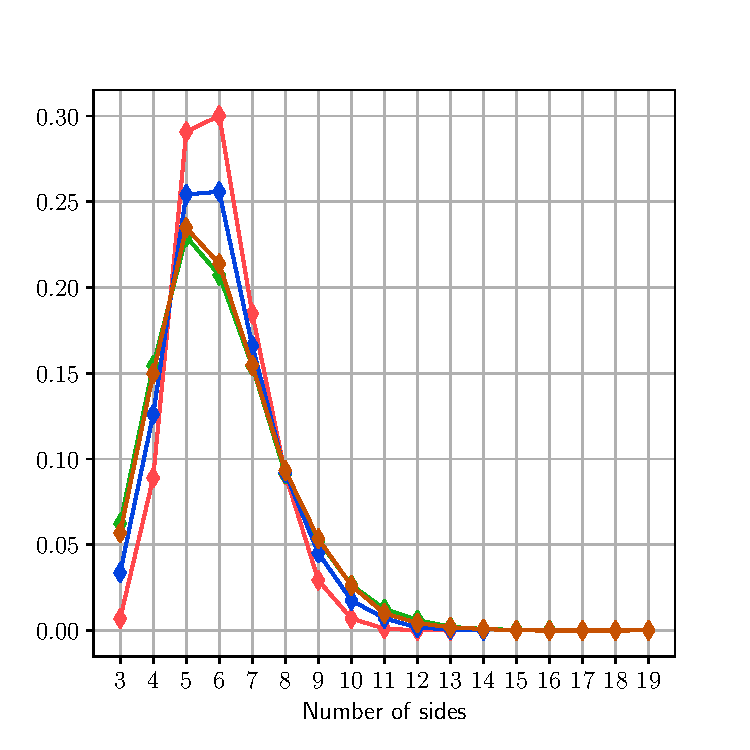
\includegraphics[trim={0 1em 0 3em},clip=true,scale=0.35]{figures/coupled_model/alt/nsides.pdf}
\end{figure}
\end{minipage}\\
\begin{minipage}{0.5\textwidth}
\begin{figure}
%    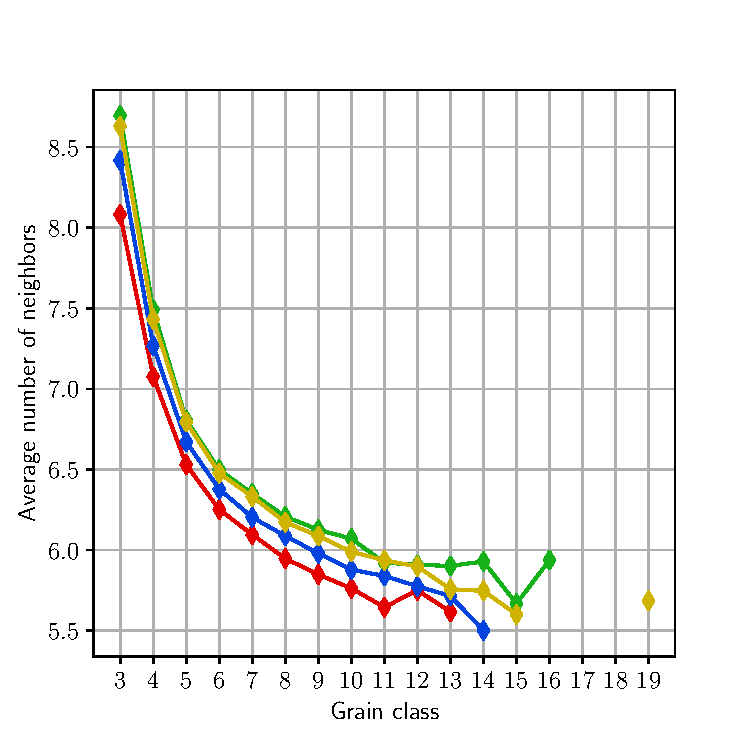
\includegraphics[trim={0 1em 0 3em},clip=true,scale=0.35]{figures/coupled_model/new_data/avg.pdf}
	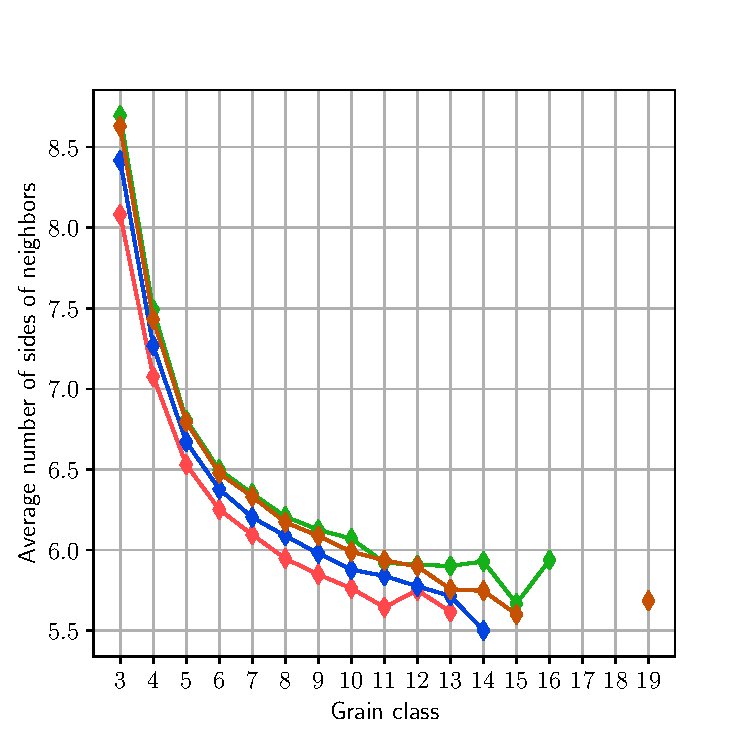
\includegraphics[trim={0 1em 0 3em},clip=true,scale=0.35]{figures/coupled_model/alt/avg.pdf}
\end{figure}
\end{minipage}%
\begin{minipage}{0.5\textwidth}
\begin{figure}
    %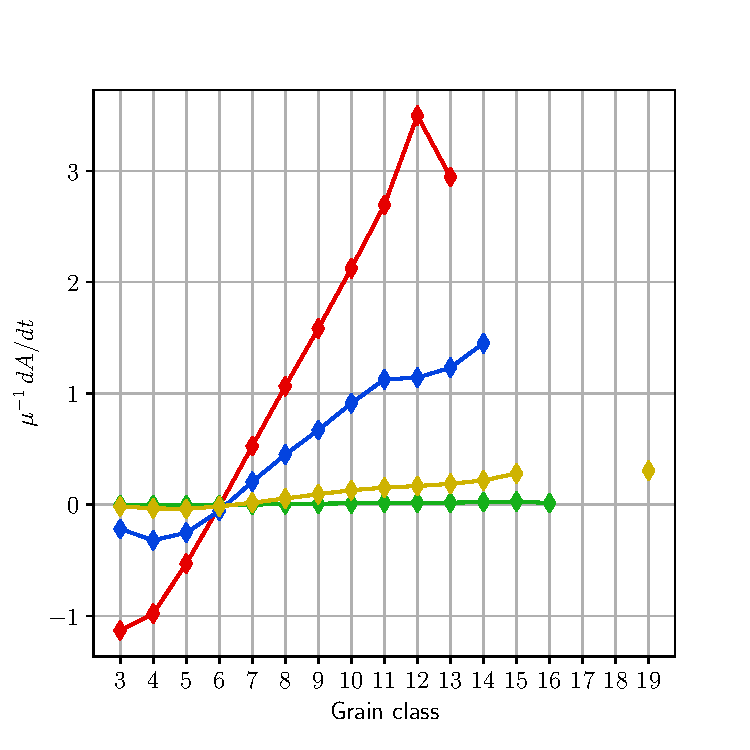
\includegraphics[trim={0 1em 0 3em},clip=true,scale=0.35]{figures/coupled_model/new_data/dAdt.pdf}
    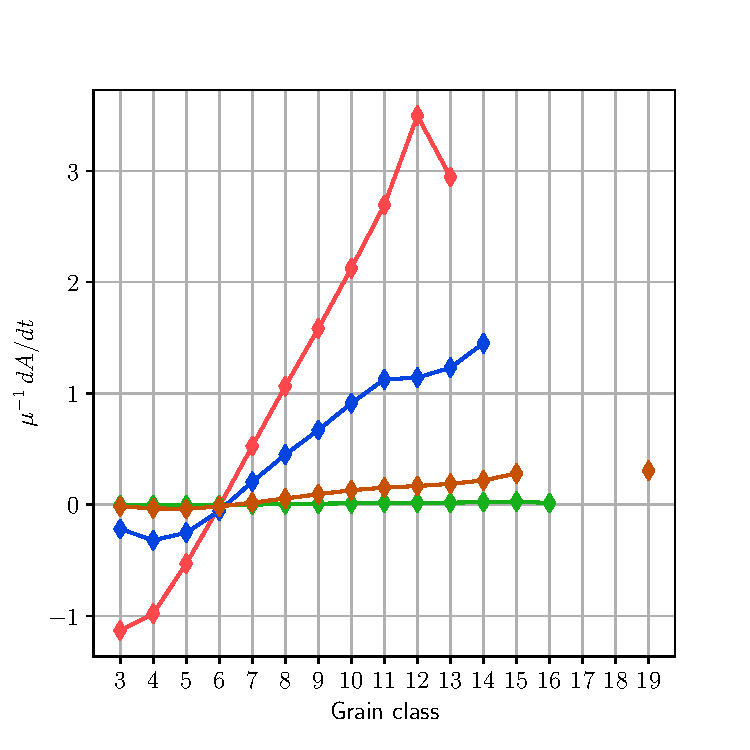
\includegraphics[trim={0 1em 0 3em},clip=true,scale=0.35]{figures/coupled_model/alt/dAdt.pdf}
\end{figure}
\end{minipage}
\end{frame}

%\begin{frame}{Numerical Experiments}
%\begin{minipage}{0.5\textwidth}
%\begin{figure}
    %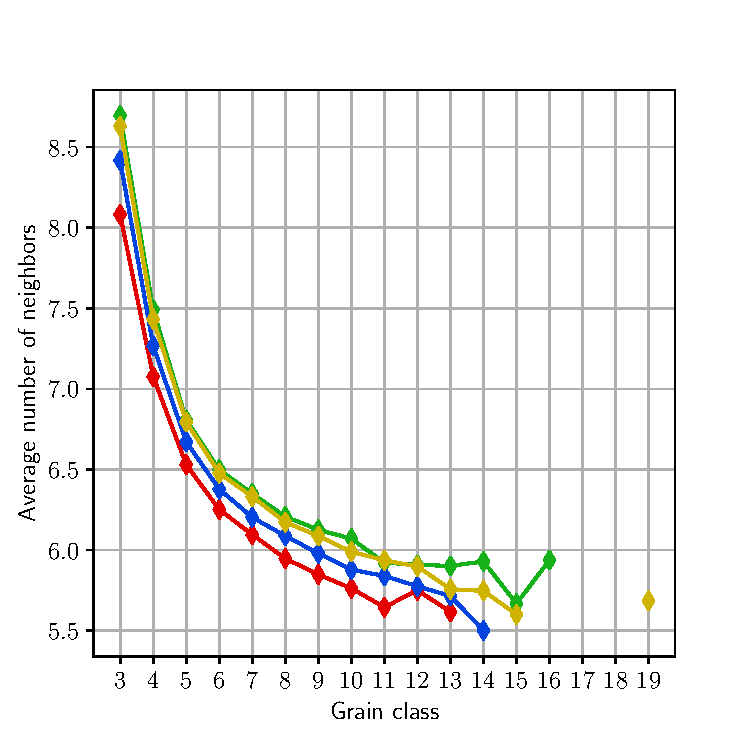
\includegraphics[scale=0.45]{figures/coupled_model/new_data/avg.pdf}
%\end{figure}
%\end{minipage}%
%\begin{minipage}{0.5\textwidth}
%\begin{figure}
    %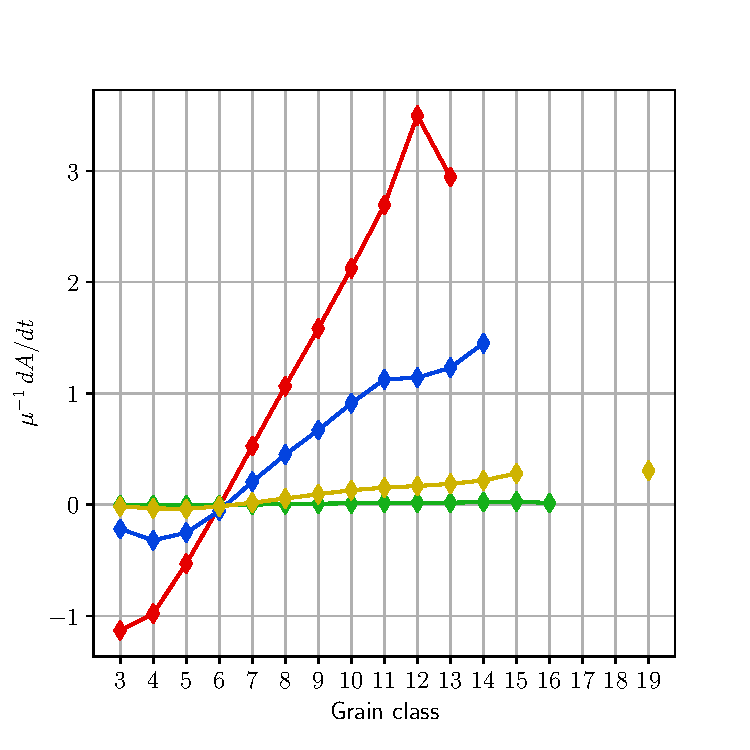
\includegraphics[scale=0.45]{figures/coupled_model/new_data/dAdt.pdf}
%\end{figure}
%\end{minipage}
%\end{frame}


\section[Stored Energy Model with Nucleation]{A Continuous Stored Energy Vertex
Model with Nucleation}

\begin{frame}{A Continuous Stored Energy Vertex
Model with Nucleation}

This extension of the Vertex Model~\cite{torres2015} considers the introduction of an stored energy term $\SE$ for each grain which plays a key role in recrystallization, that is, the nucleation of new grains~\cite{pikekos2008generalized, pikekos2008stochastic}.

We discuss the numerical algorithm for triple junction evolution, the stored energy effect on triple junctions, the nucleation process and numerical experiments.
\end{frame}


\subsection{Numerical Algorithm}
\begin{frame}{Numerical Algorithm}
\begin{minipage}{0.6\textwidth}
Consider the total energy of the system
\begin{equation*}
    E = \sum_{k=1}^K \gamma^{(k)}\AL_k + \sum_{g = 1}^N \SE_g A_g,
\end{equation*}
\end{minipage}%
\begin{minipage}{0.4\textwidth}
\begin{figure}[t]
    \centering
    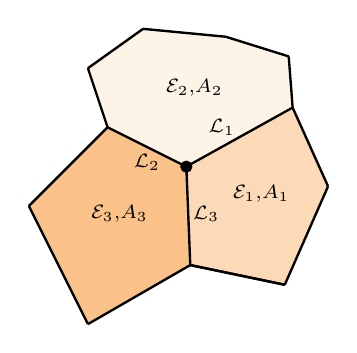
\begin{tikzpicture}[scale=0.5]
        \coordinate (v1) at (0,0);
        \coordinate (v2) at (2.7, 1.5);
        \coordinate (v3) at (3.6, -0.5);
        \coordinate (v4) at (2.5, -3);
        \coordinate (v5) at (0.1, -2.5);
        \coordinate (v6) at (-2,1);
        \coordinate (v7) at (-4, -1);
        \coordinate (v8) at (-2.5, -4);
        \coordinate (v9) at (-2.5, 2.5);
        \coordinate (v10) at (-1.1, 3.5);
        \coordinate (v11) at (1, 3.3);
        \coordinate (v12) at (2.6,2.8);
        
        % Fill perturbed area
        \fill[opacity=0.5, BurntOrange] (v1) -- (v6) -- (v7) -- (v8) -- (v5) -- cycle;
        \fill[opacity=0.3, BurntOrange] (v1) -- (v2) -- (v3) -- (v4) -- (v5) -- cycle;
          \fill[opacity=0.1, BurntOrange] (v6) -- (v9) -- (v10) -- (v11) -- (v12) -- (v2) -- (v1) -- cycle;
        
        % grain 1
        \draw[line width=0.3mm, black] (v1) -- (v2);
        \draw[line width=0.3mm, black] (v2) -- (v3);
        \draw[line width=0.3mm, black] (v3) -- (v4);
        \draw[line width=0.3mm, black] (v4) -- (v5);
        \draw[line width=0.3mm, black] (v5) -- (v1);
        % grain 2
        \draw[line width=0.3mm, black] (v4) -- (v5);
        \draw[line width=0.3mm, black] (v1) -- (v6);
        \draw[line width=0.3mm, black] (v6) -- (v7);
        \draw[line width=0.3mm, black] (v7) -- (v8);
        \draw[line width=0.3mm, black] (v8) -- (v5);
        % grain 3
        \draw[line width=0.3mm, black] (v6) -- (v9);
        \draw[line width=0.3mm, black] (v9) -- (v10);
        \draw[line width=0.3mm, black] (v10) -- (v11);
        \draw[line width=0.3mm, black] (v11) -- (v12);
        \draw[line width=0.3mm, black] (v12) -- (v2);

        \filldraw [black] (v1) circle (4pt);

        % Labels
        %\node[draw=none, color=black] at (-0.3, -0.2) {$\x_i$};
        %\node[draw=none, color=black, right] at (v2) {$\x_{j1}$};
        %\node[draw=none, color=black] at (-2.5, 1) {$\x_{j2}$};
        %\node[draw=none, color=black] at (0.1, -3) {$\x_{j3}$};
        \node[draw=none, color=black] at (0.2, 2) {$\scriptstyle \SE_2, A_2$};
        \node[draw=none, color=black] at (-1.7, -1.2) {$\scriptstyle \SE_3, A_3$};
        \node[draw=none, color=black] at (1.9, -0.7) {$\scriptstyle \SE_1, A_1$};
        
        \node[draw=none, color=Black] at (0.9,1) {$\scriptstyle \AL_1$};
        \node[draw=none, color=Black] at (-1,0.1) {$\scriptstyle \AL_2$};
        \node[draw=none, color=Black] at (0.5,-1.2) {$\scriptstyle \AL_3$};
    \end{tikzpicture}
\end{figure}
\end{minipage}

where $\gamma$ is the grain boundary energy, $\AL$ is the boundary arc length, $\SE$ is the stored energy term and $A$ is the grain area. We evolve the system by a gradient descent method. The velocity of triple junctions $\{\x_i\}$ is computed as:
\begin{equation*}
    \dotx_i = \left\langle -\frac{\partial E}{\partial x_i}, -\frac{\partial E}{\partial y_i} \right\rangle.
\end{equation*}
For this computation we use a {\color{red}matrix-free} approach. We only need to define the total energy $E$ of the system.
\end{frame}

\begin{frame}{Numerical Algorithm}
Consider the vector $\X \in \mathbb{R}^{2M}$ of stacked components of
$\x_i$, this is $
    \X = (x_1, x_2, \cdots, x_M, y_1, y_2, \cdots, y_M)^T$. Each component $m$ of the gradient of this vector, say $\partial E / \partial \X_m$ can be approximated as
\begin{equation*}
    \frac{\partial E(\X)}{\partial \X_m} \approx \frac{E(\X + \delta\,  \ei{m}) - E(\X)}{\delta},
\end{equation*}
where $\ei{m}$ is the $m$-th canonical vector in $\mathbb{R}^{2M}$. The energy of the system must be recomputed twice for each vertex where a small perturbation is added to the $m$-th component.
\end{frame}

\begin{frame}{Numerical Algorithm}
%
\begin{figure}[t]
    \centering
    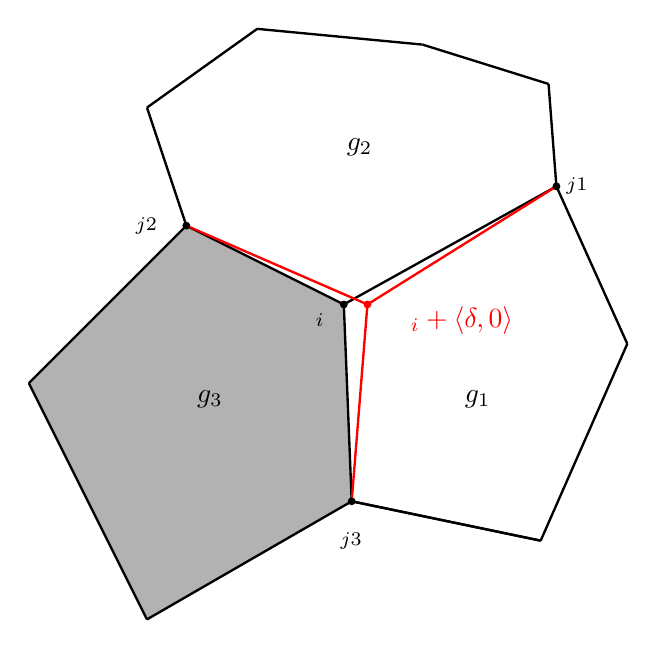
\begin{tikzpicture}
        \coordinate (v1) at (0,0);
        \coordinate (v2) at (2.7, 1.5);
        \coordinate (v3) at (3.6, -0.5);
        \coordinate (v4) at (2.5, -3);
        \coordinate (v5) at (0.1, -2.5);
        \coordinate (v6) at (-2,1);
        \coordinate (v7) at (-4, -1);
        \coordinate (v8) at (-2.5, -4);
        \coordinate (v9) at (-2.5, 2.5);
        \coordinate (v10) at (-1.1, 3.5);
        \coordinate (v11) at (1, 3.3);
        \coordinate (v12) at (2.6,2.8);
        \coordinate (pert) at ($(v1) + (0.3, 0)$);
        % grain 1
        \draw[line width=0.3mm, black] (v1) -- (v2);
        \draw[line width=0.3mm, black] (v2) -- (v3);
        \draw[line width=0.3mm, black] (v3) -- (v4);
        \draw[line width=0.3mm, black] (v4) -- (v5);
        \draw[line width=0.3mm, black] (v5) -- (v1);
        % grain 2
        \draw[line width=0.3mm, black] (v4) -- (v5);
        \draw[line width=0.3mm, black] (v1) -- (v6);
        \draw[line width=0.3mm, black] (v6) -- (v7);
        \draw[line width=0.3mm, black] (v7) -- (v8);
        \draw[line width=0.3mm, black] (v8) -- (v5);
        % grain 3
        \draw[line width=0.3mm, black] (v6) -- (v9);
        \draw[line width=0.3mm, black] (v9) -- (v10);
        \draw[line width=0.3mm, black] (v10) -- (v11);
        \draw[line width=0.3mm, black] (v11) -- (v12);
        \draw[line width=0.3mm, black] (v12) -- (v2);
        % Perturbed data
        \draw[line width=0.3mm, red] (pert) -- (v2);
        \draw[line width=0.3mm, red] (pert) -- (v6);
        \draw[line width=0.3mm, red] (pert) -- (v5);
        % vertices
        \filldraw [black] (v1) circle (1.2pt);
        \filldraw [black] (v2) circle (1.2pt);
        \filldraw [black] (v6) circle (1.2pt);
        \filldraw [black] (v5) circle (1.2pt);
        \filldraw [red] (pert) circle (1.2pt);

        % Fill perturbed area
        \fill[opacity=0.3, black] (v1) -- (v6) -- (v7) -- (v8) -- (v5) -- cycle;

        % Labels
        \node[draw=none, color=black] at (-0.3, -0.2) {$\x_i$};
        \node[draw=none, color=red] at (1.5, -0.2) {$\x_i + \langle \delta,0 \rangle$};
        \node[draw=none, color=black, right] at (v2) {$\x_{j1}$};
        \node[draw=none, color=black] at (-2.5, 1) {$\x_{j2}$};
        \node[draw=none, color=black] at (0.1, -3) {$\x_{j3}$};
        \node[draw=none, color=black] at (0.2, 2) {$g_2$};
        \node[draw=none, color=black] at (-1.7, -1.2) {$g_3$};
        \node[draw=none, color=black] at (1.7, -1.2) {$g_1$};
    \end{tikzpicture}
\end{figure}
\end{frame}


\begin{frame}[noframenumbering]{Numerical Algorithm}
 \begin{figure}[t]
     \centering
     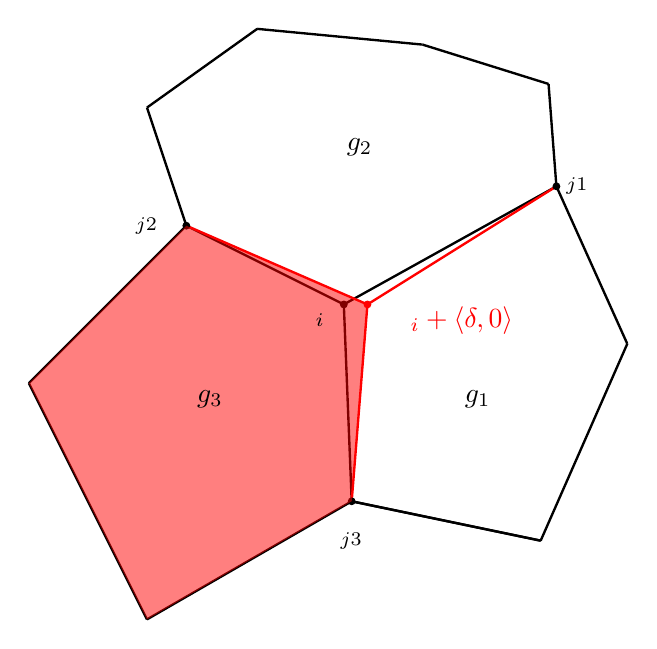
\begin{tikzpicture}
        \coordinate (v1) at (0,0);
        \coordinate (v2) at (2.7, 1.5);
        \coordinate (v3) at (3.6, -0.5);
        \coordinate (v4) at (2.5, -3);
        \coordinate (v5) at (0.1, -2.5);
        \coordinate (v6) at (-2,1);
        \coordinate (v7) at (-4, -1);
        \coordinate (v8) at (-2.5, -4);
        \coordinate (v9) at (-2.5, 2.5);
        \coordinate (v10) at (-1.1, 3.5);
        \coordinate (v11) at (1, 3.3);
        \coordinate (v12) at (2.6,2.8);
        \coordinate (pert) at ($(v1) + (0.3, 0)$);
          % grain 1
          \draw[line width=0.3mm, black] (v1) -- (v2);
          \draw[line width=0.3mm, black] (v2) -- (v3);
          \draw[line width=0.3mm, black] (v3) -- (v4);
          \draw[line width=0.3mm, black] (v4) -- (v5);
          \draw[line width=0.3mm, black] (v5) -- (v1);
          % grain 2
          \draw[line width=0.3mm, black] (v4) -- (v5);
          \draw[line width=0.3mm, black] (v1) -- (v6);
          \draw[line width=0.3mm, black] (v6) -- (v7);
          \draw[line width=0.3mm, black] (v7) -- (v8);
          \draw[line width=0.3mm, black] (v8) -- (v5);
          % grain 3
          \draw[line width=0.3mm, black] (v6) -- (v9);
          \draw[line width=0.3mm, black] (v9) -- (v10);
          \draw[line width=0.3mm, black] (v10) -- (v11);
          \draw[line width=0.3mm, black] (v11) -- (v12);
          \draw[line width=0.3mm, black] (v12) -- (v2);
          % Perturbed data
          \draw[line width=0.3mm, red] (pert) -- (v2);
          \draw[line width=0.3mm, red] (pert) -- (v6);
          \draw[line width=0.3mm, red] (pert) -- (v5);
          % vertices
          \filldraw [black] (v1) circle (1.2pt);
          \filldraw [black] (v2) circle (1.2pt);
          \filldraw [black] (v6) circle (1.2pt);
          \filldraw [black] (v5) circle (1.2pt);
          \filldraw [red] (pert) circle (1.2pt);

          % Fill perturbed area
          \fill[opacity=0.5, red] (pert) -- (v6) -- (v7) -- (v8) -- (v5) -- cycle;

          % Labels
          \node[draw=none, color=black] at (-0.3, -0.2) {$\x_i$};
          \node[draw=none, color=red] at (1.5, -0.2) {$\x_i + \langle \delta,0 \rangle$};
          %\node[draw=none, color=black] at (3.5, 0.6) {$\x_{j1}$};
          \node[draw=none, color=black, right] at (v2) {$\x_{j1}$};
          \node[draw=none, color=black] at (-2.5, 1) {$\x_{j2}$};
          \node[draw=none, color=black] at (0.1, -3) {$\x_{j3}$};
          \node[draw=none, color=black] at (0.2, 2) {$g_2$};
          \node[draw=none, color=black] at (-1.7, -1.2) {$g_3$};
          \node[draw=none, color=black] at (1.7, -1.2) {$g_1$};
     \end{tikzpicture}
  \end{figure}
\end{frame}

\begin{frame}{Numerical Algorithm}
Since we are perturbing only three arc lengths and there grain areas, we do not need to recompute the total energy but only the difference of energies:
\begin{align*}
    E(\X+\delta\,  \ei{m}) - E(\X) &=
    \sum_{k =1}^K \gamma^{(k)}\Delta{\AL}_{k} +
     \sum_{g=1}^N \SE_{g}\Delta{A}_{g}\\
    &= \sum_{j=1}^3 \gamma^{(k_{i,j})} \Delta \AL_{k_{i,j}} + \sum_{j=1}^3 \SE_{g_{i,j}} \Delta A_{g_{i,j}},
\end{align*}
Therefore,
\begin{equation*}
    \frac{\partial E(\X)}{\partial \X_m} \approx
    \frac{E(\X+\delta\,  \ei{m}) - E(\X)}{\delta} = \sum_{j=1}^3 \gamma^{(k_{i,j})}  \frac{\Delta \AL_{k_{i,j}}}{\delta}+ \sum_{j=1}^3 \SE_{g_{i,j}} \frac{\Delta A_{g_{i,j}}}{\delta}.
\end{equation*}
\end{frame}

%%%%%%%%%%%%%%%%%%%%%%%%%%%%%%%%%%%%%%%%%%%%%%%%%%%%%%%%%%%%%%%

\subsection[Effect of Stored Energy over TJ]{Effect of Stored Energy over TJ Evolution}
\begin{frame}{Effect of Stored Energy over TJ Evolution}
    Consider the following domain $[a \times b]$ with isotropic grain setting:
    \begin{figure}
        \centering
        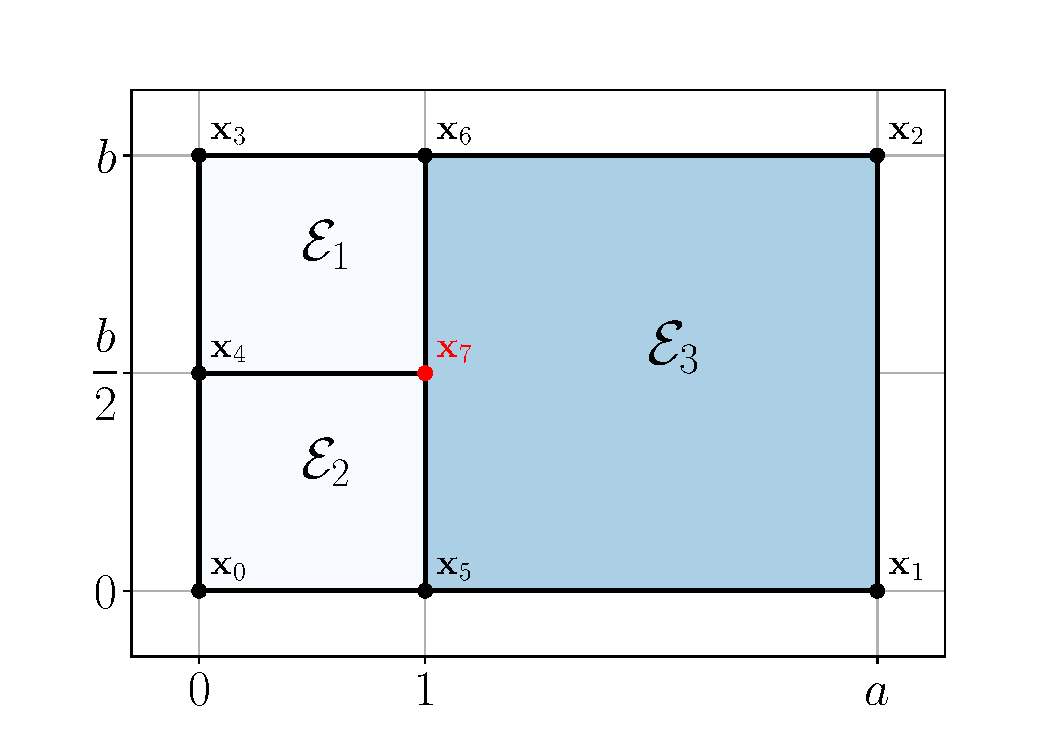
\includegraphics[trim={1em 2em 1em 3em}, clip=true, scale=0.5]{figures/stored_energy/SE_analysis.pdf}
    \end{figure}
    where $\SE_1, \SE_2$ and $\SE_3$ are the stored energies for each grain.

    The triple junction {\color{red}$\x_7$} can freely move along x-axis.
\end{frame}


% \begin{frame}{Effect of Stored Energy over TJ Evolution}
%     Let's suppose $\SE_1 = \SE_2$. The steady state of {\color{red} $\x_7$} depends on $\Delta \SE = \SE_3 - \SE_1$.
%     The analysis of the steady state of {\color{red} $\x_7$} shows that stable configurations can be found for $b\Delta \SE < 6$.
%     \begin{figure}
%         \centering
%         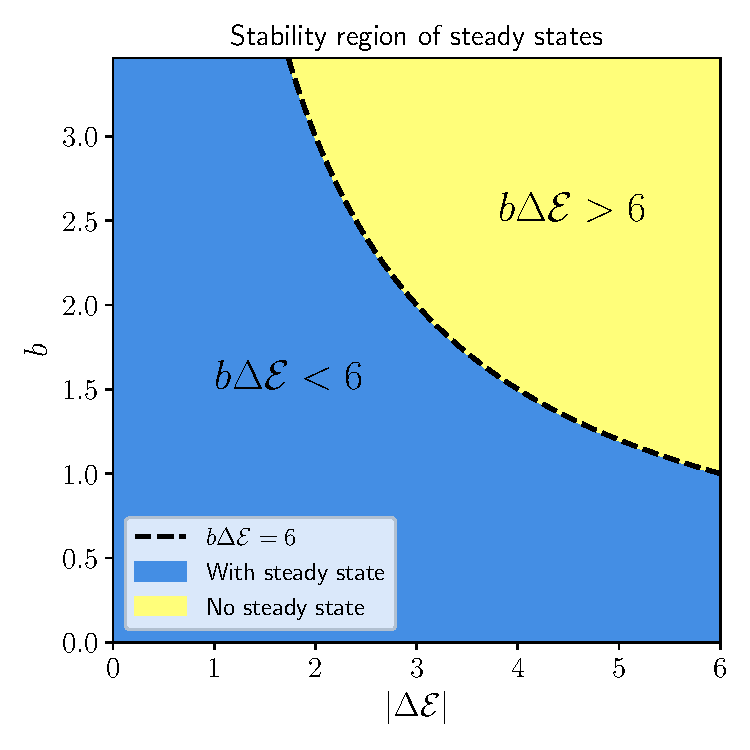
\includegraphics[scale=0.48]{figures/stored_energy/SE_stability.pdf}
%     \end{figure}
% \end{frame}


\begin{frame}{Effect of Stored Energy over TJ Evolution}
    %\vspace{-0.5em}
    \begin{tabular}{m{0.46\textwidth} m{0.50\textwidth}}
    If $\Delta \SE = 0$ the steady state of {\color{red} $\x_7$} is at $x = 1 - \frac{b}{2\sqrt{3}}$. Here the dihedral angles stays at $2\pi/3$.
     & 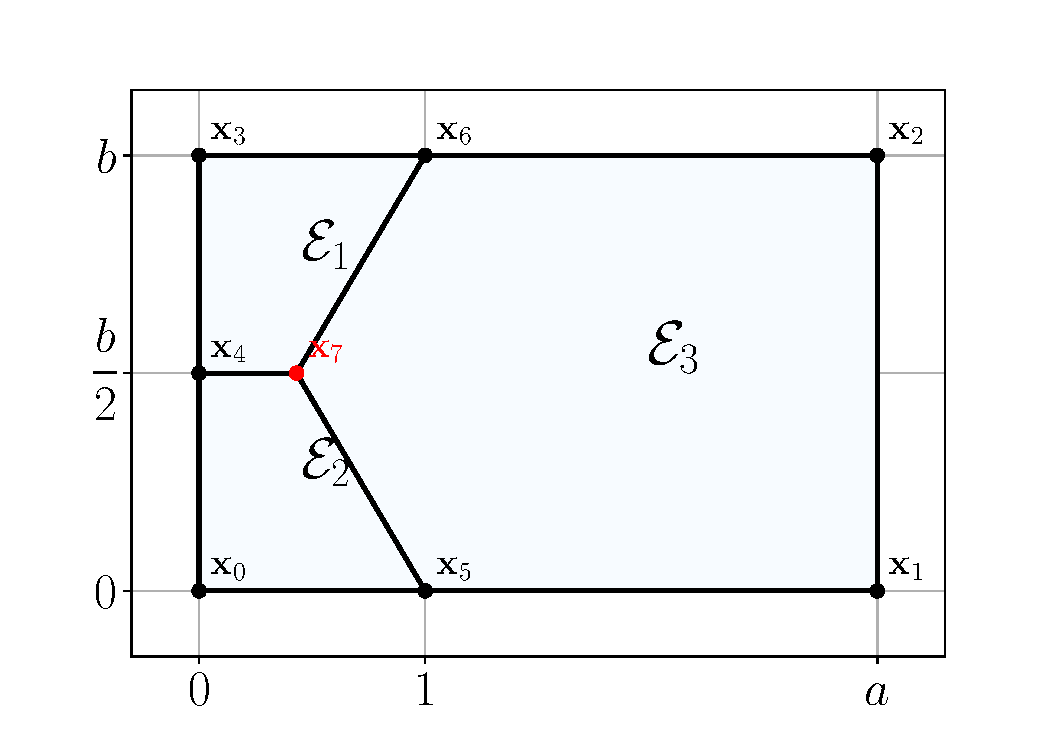
\includegraphics[trim={1em 2em 1em 3em}, clip=true,,scale=0.35]{figures/stored_energy/SE_analysis_SE0.pdf}\\
    %\vspace{-0.5em}
    If $0 < \Delta \SE < 6$ the steady state {\color{red} $\x_7$} will move towards
    the grain with high stored energy value. & 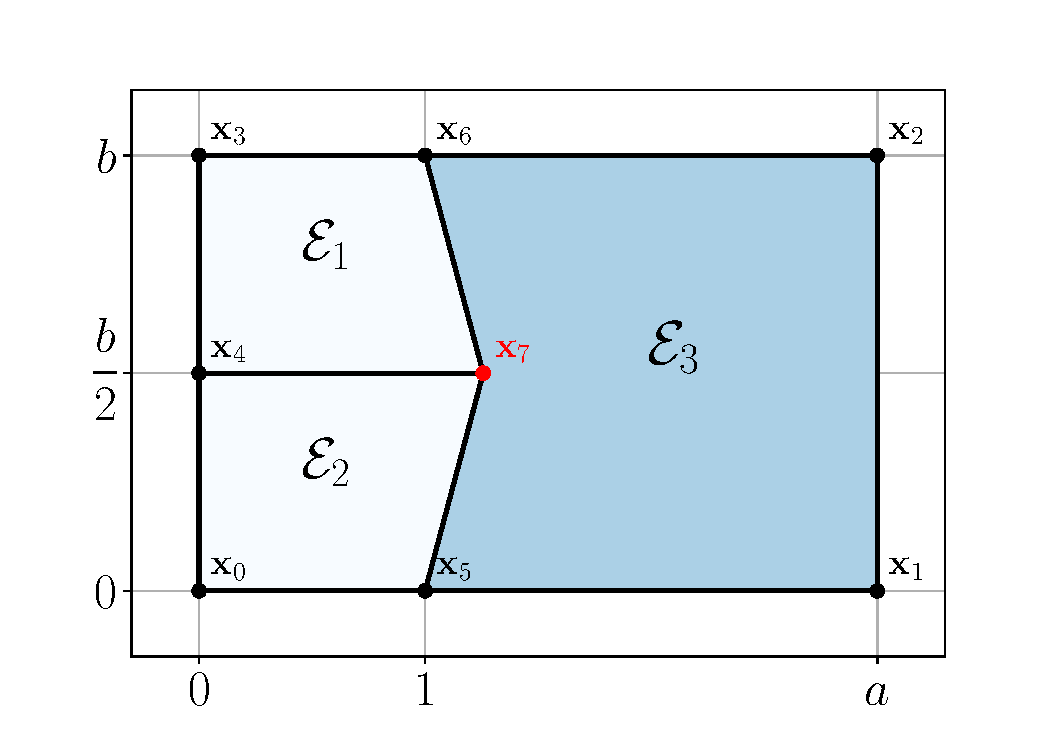
\includegraphics[trim={1em 2em 1em 3em}, clip=true,scale=0.35]{figures/stored_energy/SE_analysis_SE1dot5.pdf}
    \end{tabular}
\end{frame}

% \begin{frame}{Effect of Stored Energy over TJ Evolution}
%     If $\Delta \SE \geq 6$ the are no steady states and solutions for {\color{red} $\x_7$} becomes unbounded.
%     \begin{figure}
%         \centering
%         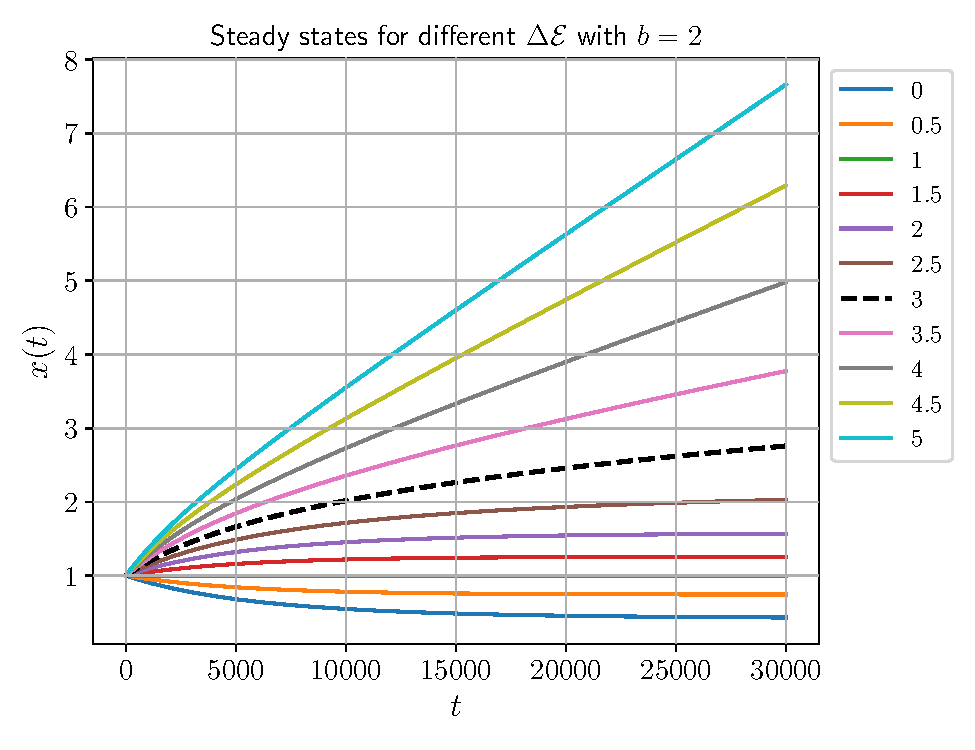
\includegraphics[trim={1em 1em 1em 1em}, clip=true,scale=0.4]{figures/stored_energy/SE_experiments.pdf}
%     \end{figure}
%     This estimation can be used as an upper bound for numerical simulations of this model, ensuring that no grains will suffer from instabilities.
%     The interpretation is that the parameter $b$ of this study can be compared to boundaries arc lengths.
% \end{frame}

\begin{frame}{Effect of Stored Energy over TJ Evolution}
The analysis of the steady state of {\color{red} $\x_7$} shows that stable configurations can be found for $b\Delta \SE < 6$.
\begin{figure}
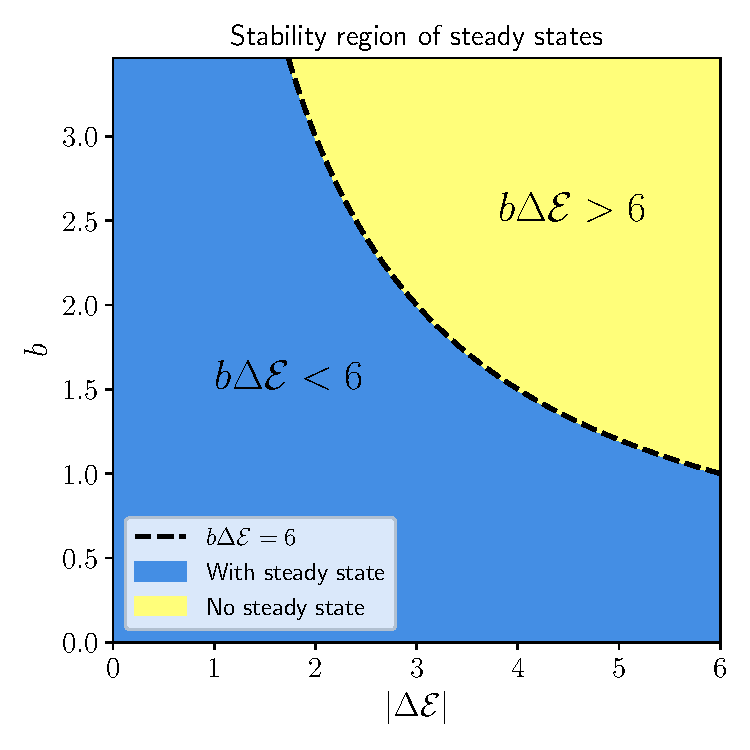
\includegraphics[scale=0.38,valign=t, trim={0 0 0 1em}]{figures/stored_energy/SE_stability.pdf}\hfill
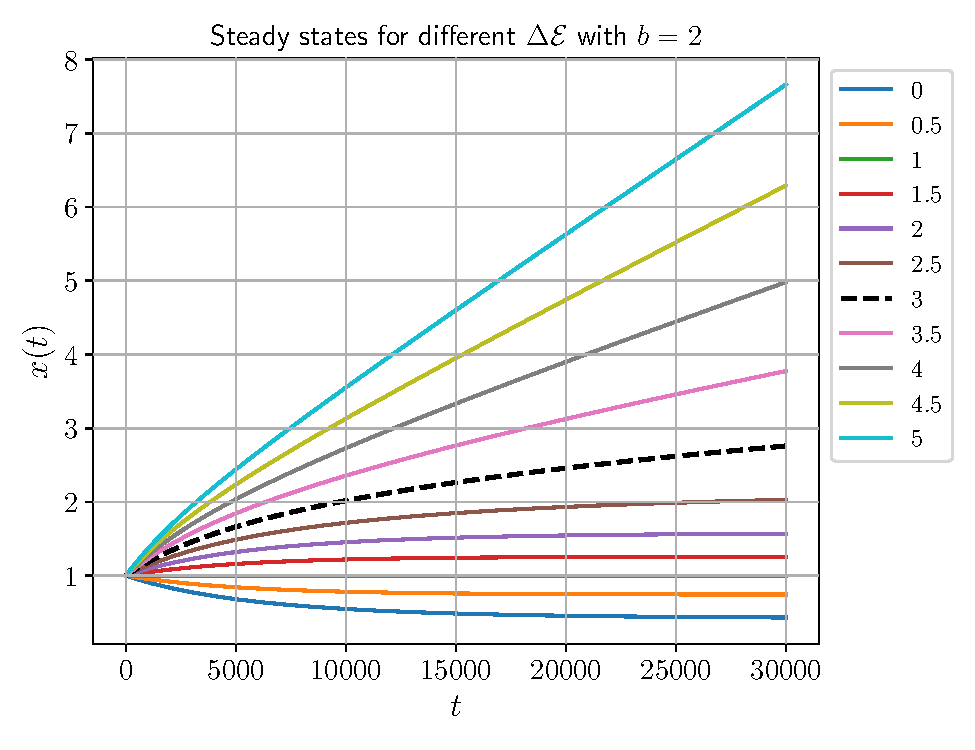
\includegraphics[trim={1em 1em 1em 1em}, clip=true,scale=0.38,valign=t]{figures/stored_energy/SE_experiments.pdf}
\end{figure}
%This estimation can be used as an upper bound for numerical simulations of this model, ensuring that no grains will suffer from instabilities.
%The interpretation is that the parameter $b$ of this study can be compared to boundaries arc lengths.
\end{frame}

\subsection{The Nucleation Process}
\begin{frame}{The Nucleation Process}
    This topological transition adds a new grain at a specific vertex. Consider the vertex $\x_1$ and its neighbors $\{\x_2, \x_3, \x_4\}$. We will add a grain at this \emph{candidate site} and analyze whether if it will grow or shrink.
    \begin{figure}[t]
    \centering
    \begin{minipage}{0.3\textwidth}
        \centering
        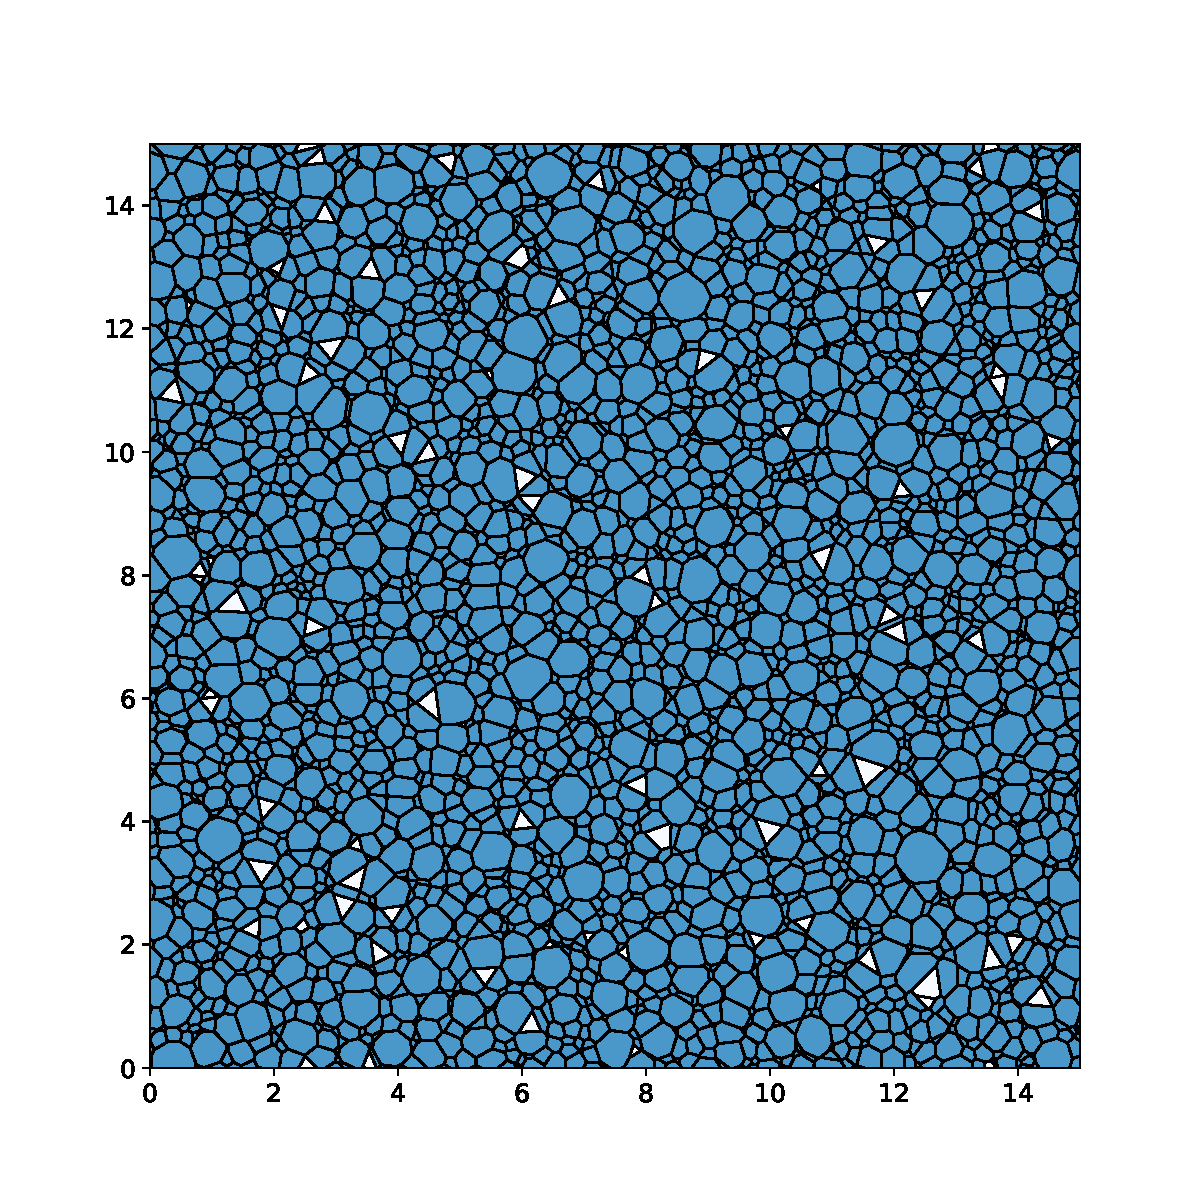
\includegraphics[trim={8cm 8cm 8cm 8cm},clip=true,scale=0.8]{figures/stored_energy/SE/snaps/000070.pdf}
    \end{minipage}%
    \begin{minipage}{0.25\textwidth}
        \centering
        \begin{turn}{60}
        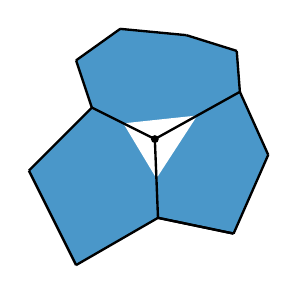
\begin{tikzpicture}[scale=0.4]
            \coordinate (v1) at (0,0);
            \coordinate (v2) at (2.7, 1.5);
            \coordinate (v3) at (3.6, -0.5);
            \coordinate (v4) at (2.5, -3);
            \coordinate (v5) at (0.1, -2.5);
            \coordinate (v6) at (-2,1);
            \coordinate (v7) at (-4, -1);
            \coordinate (v8) at (-2.5, -4);
            \coordinate (v9) at (-2.5, 2.5);
            \coordinate (v10) at (-1.1, 3.5);
            \coordinate (v11) at (1, 3.3);
            \coordinate (v12) at (2.6,2.8);
            
            \coordinate (a1) at ($0.5*(v1)+0.5*(v2)$);
            \coordinate (a2) at ($0.5*(v1)+0.5*(v6)$);
            \coordinate (a3) at ($0.5*(v1)+0.5*(v5)$);
            
            % Fill perturbed area
            \fill[bluegrain] (v1) -- (v6) -- (v7) -- (v8) -- (v5) -- cycle;
            \fill[bluegrain] (v1) -- (v2) -- (v3) -- (v4) -- (v5) -- cycle;
            \fill[bluegrain] (v6) -- (v9) -- (v10) -- (v11) -- (v12) -- (v2) -- (v1) -- cycle;
            
             \fill[white] (a1) -- (a2) -- (a3) -- cycle;
            
            % grain 1
            \draw[line width=0.3mm, black] (v1) -- (v2);
            \draw[line width=0.3mm, black] (v2) -- (v3);
            \draw[line width=0.3mm, black] (v3) -- (v4);
            \draw[line width=0.3mm, black] (v4) -- (v5);
            \draw[line width=0.3mm, black] (v5) -- (v1);
            % grain 2
            \draw[line width=0.3mm, black] (v4) -- (v5);
            \draw[line width=0.3mm, black] (v1) -- (v6);
            \draw[line width=0.3mm, black] (v6) -- (v7);
            \draw[line width=0.3mm, black] (v7) -- (v8);
            \draw[line width=0.3mm, black] (v8) -- (v5);
            % grain 3
            \draw[line width=0.3mm, black] (v6) -- (v9);
            \draw[line width=0.3mm, black] (v9) -- (v10);
            \draw[line width=0.3mm, black] (v10) -- (v11);
            \draw[line width=0.3mm, black] (v11) -- (v12);
            \draw[line width=0.3mm, black] (v12) -- (v2);
    
            \filldraw [black] (v1) circle (3pt);
        \end{tikzpicture}
        \end{turn}
    \end{minipage}\hspace{3em}%
    \begin{minipage}{0.3\textwidth}
        \centering
        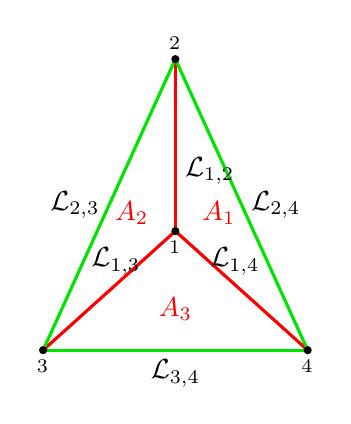
\begin{tikzpicture}[scale=0.84]
        % coordinates
        \coordinate (x1) at (0,-0.5);
        \coordinate (x2) at (0,2.1);
        \coordinate (x3) at (-2,-2.3);
        \coordinate (x4) at (2, -2.3);
        % boundaries
        \draw[line width=0.4mm, red] (x1) -- (x2);
        \draw[line width=0.4mm, red] (x1) -- (x3);
        \draw[line width=0.4mm, red] (x1) -- (x4);
        \draw[line width=0.4mm, black!10!green] (x2) -- (x3);
        \draw[line width=0.4mm, black!10!green] (x3) -- (x4);
        \draw[line width=0.4mm, black!10!green] (x2) -- (x4);

        % vertices
        \filldraw [black] (x1) circle (1.5pt);
        \filldraw [black] (x2) circle (1.5pt);
        \filldraw [black] (x3) circle (1.5pt);
        \filldraw [black] (x4) circle (1.5pt);

        % Text
        \node[draw=none, color=black, below] at (x1) {$\x_{1}$};
        \node[draw=none, color=black, above] at (x2) {$\x_{2}$};
        \node[draw=none, color=black, below] at (x3) {$\x_{3}$};
        \node[draw=none, color=black, below] at (x4) {$\x_{4}$};

        \node[draw=none, color=black, right] at ($(x2)!0.5!(x4)$) {$\AL_{2,4}$};
        \node[draw=none, color=black,left] at ($(x2)!0.5!(x3)$) {$\AL_{2,3}$};
        \node[draw=none, color=black, below] at ($(x3)!0.5!(x4)$) {$\AL_{3,4}$};

        \node[draw=none, color=black, right] at ($(x1)!0.35!(x2)$) {$\AL_{1,2}$};
        \node[draw=none, color=black, above] at ($(x1)!0.45!(x3)$) {$\AL_{1,3}$};
        \node[draw=none, color=black, above] at ($(x1)!0.45!(x4)$) {$\AL_{1,4}$};

        \node[draw=none, color=black] at ($0.33*(x1)+0.33*(x4)+0.33*(x2)$) {$\color{red}{A_{1}}$};
        \node[draw=none, color=black] at ($0.33*(x1)+0.33*(x2)+0.33*(x3)$) {$\color{red}{A_{2}}$};
        \node[draw=none, color=black] at ($0.33*(x1)+0.33*(x3)+0.33*(x4)$) {$\color{red}{A_{3}}$};
        \end{tikzpicture}
    \end{minipage}
    \end{figure}

    Consider the energy prior to nucleation $E_0^{\triangle}$ and the candidate energy $E_1^{\triangle}$. We need $\Delta E^{\triangle} = E_1^{\triangle} - E_0^{\triangle} < 0$ to ensure growth.
\end{frame}

\begin{frame}{The Nucleation Process - Symmetric Case}
\begin{minipage}{0.5\textwidth}
Consider each arc length $\AL_{1,i} = r$ and $\AL_{2,3}=\AL_{2,4}=\AL_{3,4}=L$ and dihedral angle $2\pi/3$. The energy difference simplifies to:
\begin{equation*}
    \Delta E^{\triangle} = 3\,r\,\left(\sqrt{3}-1-\frac{\sqrt{3}}{12}\,\bar{\SE}\,r\right).
\end{equation*}
 The critical points of $\Delta E$ are:
\begin{equation*}
     r_0 = 0\quad\text{and}\quad r_c = \dfrac{4\,(3 - \sqrt{3})}{\bar{\SE}}%\approx \frac{5.071796}{\bar{\SE}}
\end{equation*}
\end{minipage}\hfill
\begin{minipage}{0.45\textwidth}
\begin{figure}
    \centering
    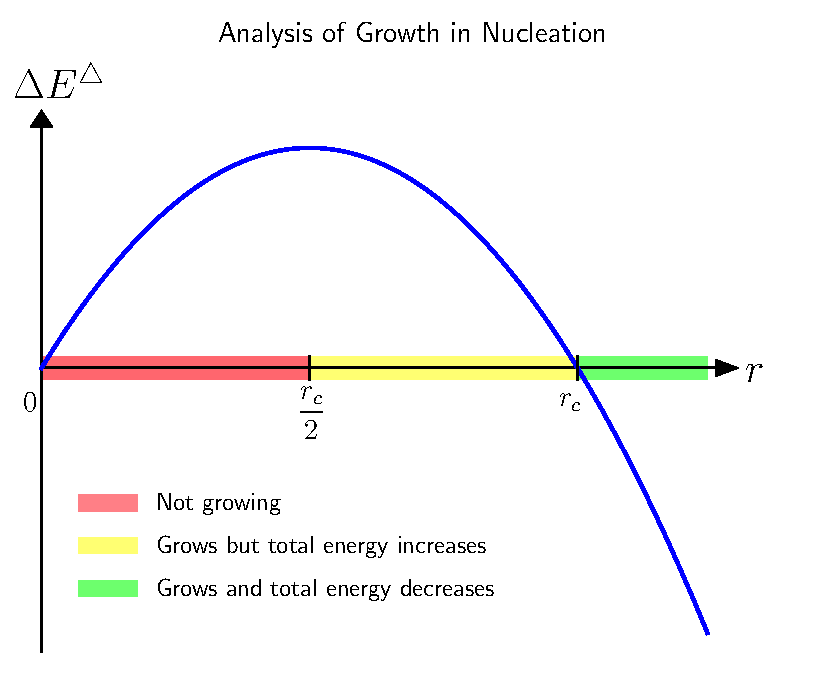
\includegraphics[trim={0 1em 0 2.5em},clip=true,scale=0.44]{figures/stored_energy/DeltaETriangle.pdf}
\end{figure}
\end{minipage}\\
\begin{minipage}{\textwidth}
\vspace{1em}
We will look at the slope of the plot, that is $\Delta(\Delta E^{\triangle}):= \Delta^2E^{\triangle}$.
\end{minipage}
% \begin{equation*}
%     \Delta E^{\triangle} = 3L - 3r - \underbrace{(\SE_1 + \SE_2 + \SE_3)}_{\displaystyle{\bar{\SE}}}A.
% \end{equation*}
% By symmetry the energy difference becomes:

% The critical points of $\Delta E$ are:
% \begin{equation*}
%     r_0 = 0\quad\text{and}\quad r_c = \dfrac{4\,(3 - \sqrt{3})}{\bar{\SE}}\approx \frac{5.071796}{\bar{\SE}}
% \end{equation*}
\end{frame}

% \begin{frame}{The Nucleation Process - Symmetric Case}
% The interesting case is $r_c$ since will allow a grain to grow without increasing the energy of the system.
% \begin{figure}
%     \centering
%     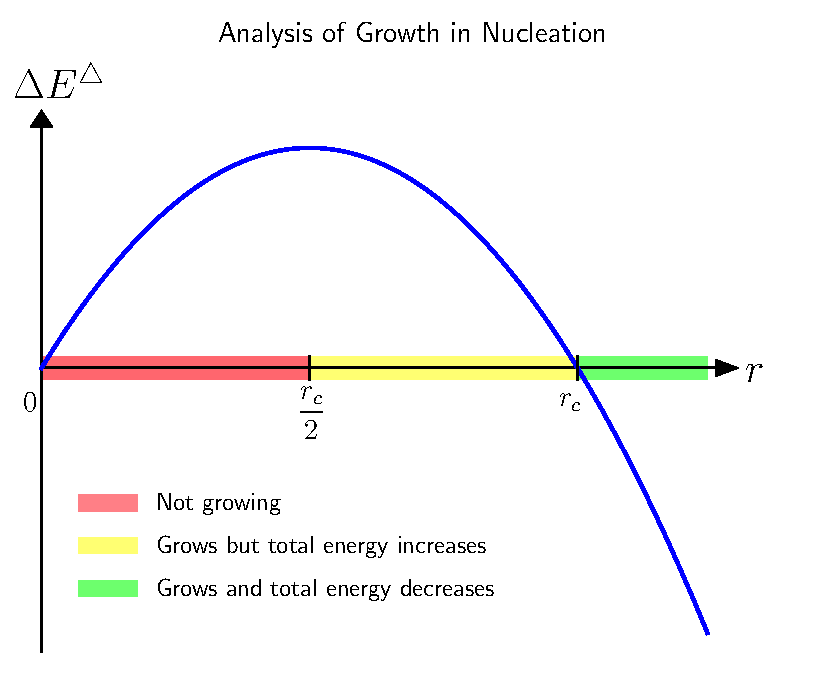
\includegraphics[trim={0 1em 0 2.5em},clip=true,scale=0.45]{figures/stored_energy/DeltaETriangle.pdf}
% \end{figure}
% If we choose $r > r_c/2$ we ensure growth. if we choose $r > r_c$ we also ensure decreasing energy. We will look at the slope of the plot, that is $\Delta(\Delta E^{\triangle}):= \Delta^2E^{\triangle}$
% \end{frame}

\begin{frame}{The Nucleation Process - Symmetric Case}
We estimate $\Delta^2E^{\triangle} = \Delta E^{\triangle}_1 - \Delta E^{\triangle}_0$ by performing virtual nucleations.
\begin{figure}[t]
    \centering
    \subfloat[$\Delta E^{\triangle}_1$] {
    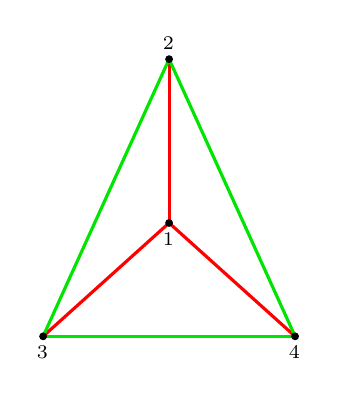
\begin{tikzpicture}[scale=0.8]
        % coordinates
        \coordinate (x1) at (0,-0.5);
        \coordinate (x2) at (0,2.1);
        \coordinate (x3) at (-2,-2.3);
        \coordinate (x4) at (2, -2.3);
        % boundaries
        \draw[line width=0.4mm, red] (x1) -- (x2);
        \draw[line width=0.4mm, red] (x1) -- (x3);
        \draw[line width=0.4mm, red] (x1) -- (x4);
        \draw[line width=0.4mm, black!10!green] (x2) -- (x3);
        \draw[line width=0.4mm, black!10!green] (x3) -- (x4);
        \draw[line width=0.4mm, black!10!green] (x2) -- (x4);

        % vertices
        \filldraw [black] (x1) circle (1.5pt);
        \filldraw [black] (x2) circle (1.5pt);
        \filldraw [black] (x3) circle (1.5pt);
        \filldraw [black] (x4) circle (1.5pt);

        % Text
        \node[draw=none, color=black, below] at (x1) {$\x_{1}$};
        \node[draw=none, color=black, above] at (x2) {$\x_{2}$};
        \node[draw=none, color=black, below] at (x3) {$\x_{3}$};
        \node[draw=none, color=black, below] at (x4) {$\x_{4}$};

    \end{tikzpicture}
    \label{fig:delta2_1}
    }\hspace{5em}
    \subfloat[$\Delta E^{\triangle}_0$] {
    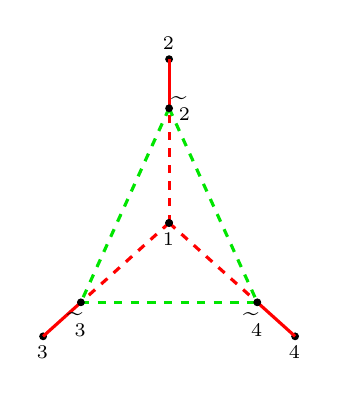
\begin{tikzpicture}[scale=0.8]
        % coordinates
        \coordinate (x1) at (0,-0.5);
        \coordinate (x2) at (0,2.1);
        \coordinate (x3) at (-2,-2.3);
        \coordinate (x4) at (2, -2.3);

        % vertices
        \filldraw [black] (x1) circle (1.5pt);
        \filldraw [black] (x2) circle (1.5pt);
        \filldraw [black] (x3) circle (1.5pt);
        \filldraw [black] (x4) circle (1.5pt);

        %%%%%%%%%%%%%%%%%%%%%%%%%%%%%%%%%%%%%%%%%%%%%
        % coordinates
        \coordinate (x12) at (x1);
        \coordinate (x22) at ($(x2)!0.3!(x1)$);
        \coordinate (x32) at ($(x3)!0.3!(x1)$);
        \coordinate (x42) at ($(x4)!0.3!(x1)$);

        % boundaries
        \draw[line width=0.4mm, red] (x22) -- (x2);
        \draw[line width=0.4mm, red, dashed] (x1) -- (x22);
        \draw[line width=0.4mm, red] (x32) -- (x3);
        \draw[line width=0.4mm, red, dashed] (x1) -- (x32);
        \draw[line width=0.4mm, red] (x42) -- (x4);
        \draw[line width=0.4mm, red, dashed] (x1) -- (x42);
        % boundaries
        \draw[line width=0.4mm, black!10!green, dashed] (x22) -- (x32);
        \draw[line width=0.4mm, black!10!green, dashed] (x32) -- (x42);
        \draw[line width=0.4mm, black!10!green, dashed] (x22) -- (x42);

        % vertices
        \filldraw [black] (x12) circle (1.5pt);
        \filldraw [black] (x22) circle (1.5pt);
        \filldraw [black] (x32) circle (1.5pt);
        \filldraw [black] (x42) circle (1.5pt);

        % Text
        \node[draw=none, color=black, below] at (x1) {$\x_{1}$};
        \node[draw=none, color=black, above] at (x2) {$\x_{2}$};
        \node[draw=none, color=black, below] at (x3) {$\x_{3}$};
        \node[draw=none, color=black, below] at (x4) {$\x_{4}$};

        % Text
        \node[draw=none, color=black, right] at (x22) {$\widetilde{\x}_{2}$};
        \node[draw=none, color=black, below] at (x32) {$\widetilde{\x}_{3}$};
        \node[draw=none, color=black, below] at (x42) {$\widetilde{\x}_{4}$};

    \end{tikzpicture}
    \label{fig:delta2_2}
    }
\end{figure}
We call $\Delta^2 E^{\triangle}$ the \emph{nucleation factor}. We compute it for each vertex and we choose the site with the minimum negative value.
\end{frame}

\begin{frame}{The Nucleation Process - Orientations}
    In practice we need to choose an orientation for the nucleated grain.
    \begin{itemize}
        \item The {\color{red}basic nucleation} considers orientation $\alpha = 0$.
        \item The {\color{blue}alternative nucleation} considers a local optimization choosing an orientation as $\alpha = \min_{\widehat{\alpha} \in [0,2\pi)} E_1^\triangle$, that is, we minimize the energy introduced by nucleation.
    \end{itemize}
\end{frame}

\subsection{Numerical Experiments}

\begin{frame}{Numerical Experiments}
      \centering
   \movie[width=\textwidth,height=\textheight]{Simulation}{/home/asazo/Escritorio/se.mov}
\end{frame}

\begin{frame}{Energy Behavior}
We compared the energy behavior by nucleating grains with the two described orientation choices.
\begin{minipage}{0.5\textwidth}
\vspace{1em}
\begin{figure}
    \centering
    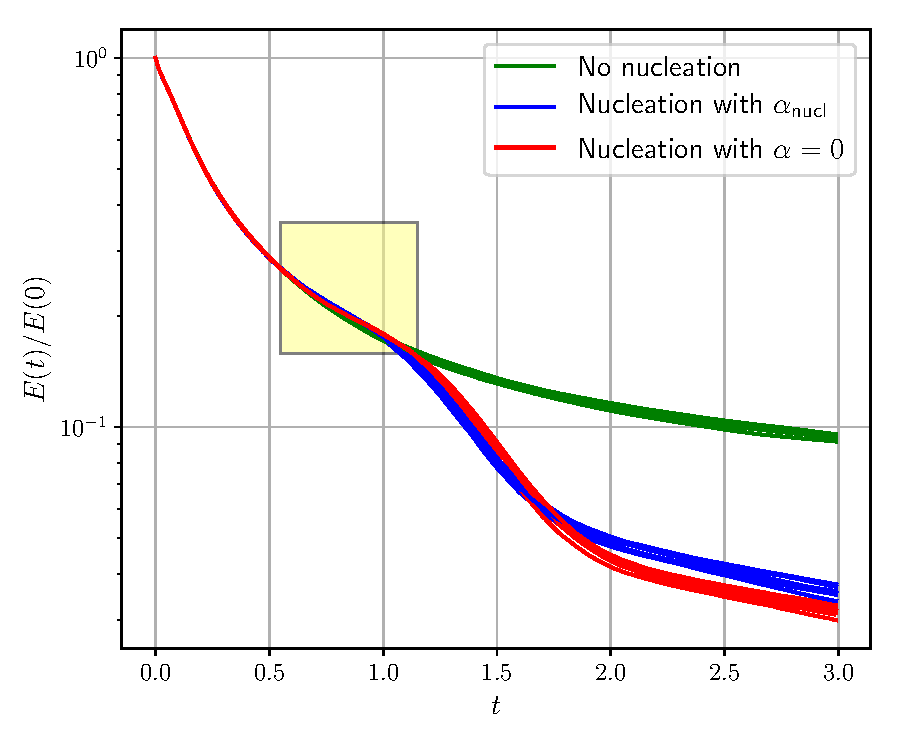
\includegraphics[scale=0.4]{figures/stored_energy/SE_energy.pdf}
\end{figure}
\end{minipage}%
\begin{minipage}{0.5\textwidth}
\vspace{1em}
\begin{figure}
    \centering
    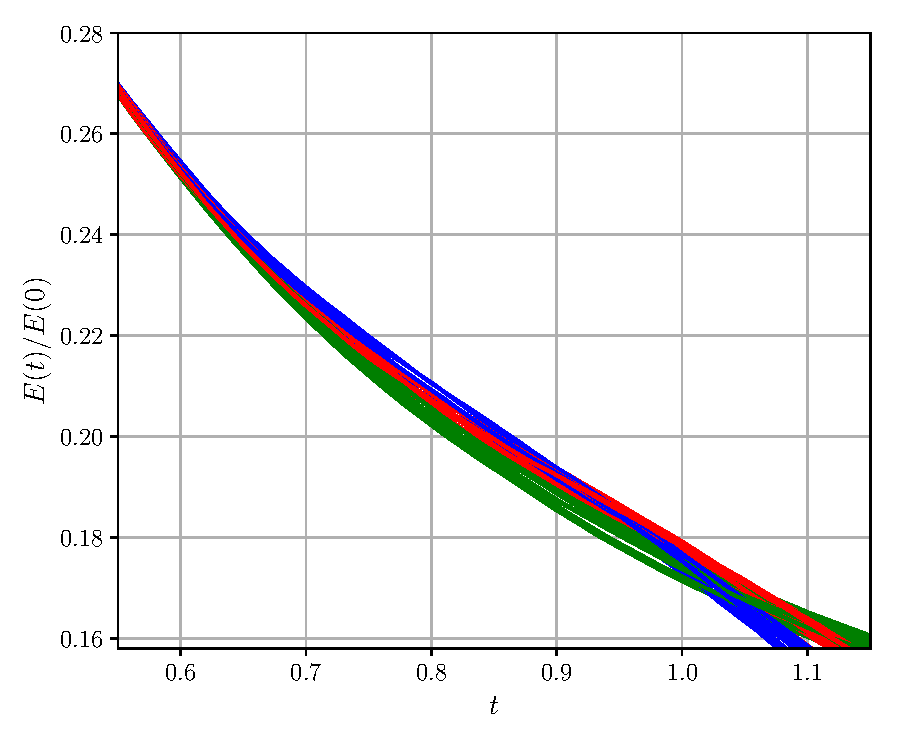
\includegraphics[scale=0.4]{figures/stored_energy/SE_energy_zoom.pdf}
\end{figure}
\end{minipage}
\end{frame}

\begin{frame}{Statistics - Nucleation $\alpha = 0$ - Relative area}
\small
\centering
    \vspace{-0.5em}
    \begin{figure}
        \centering
        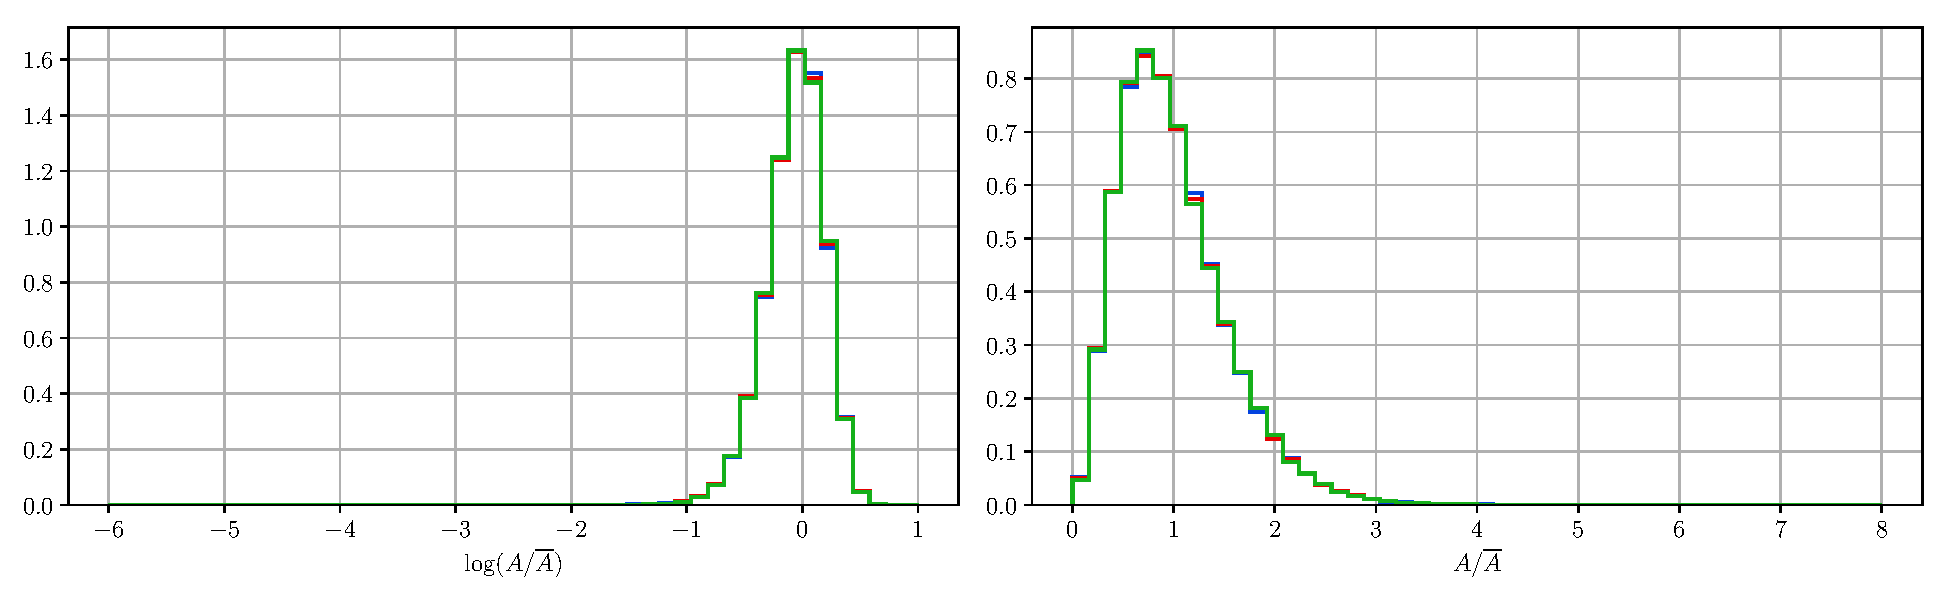
\includegraphics[scale=0.35]{figures/stored_energy/SE/areas/000000_nuclconstant_set.pdf}
    \end{figure}
    \vspace{-1em}
    Initial condition
    \begin{figure}
        \centering
        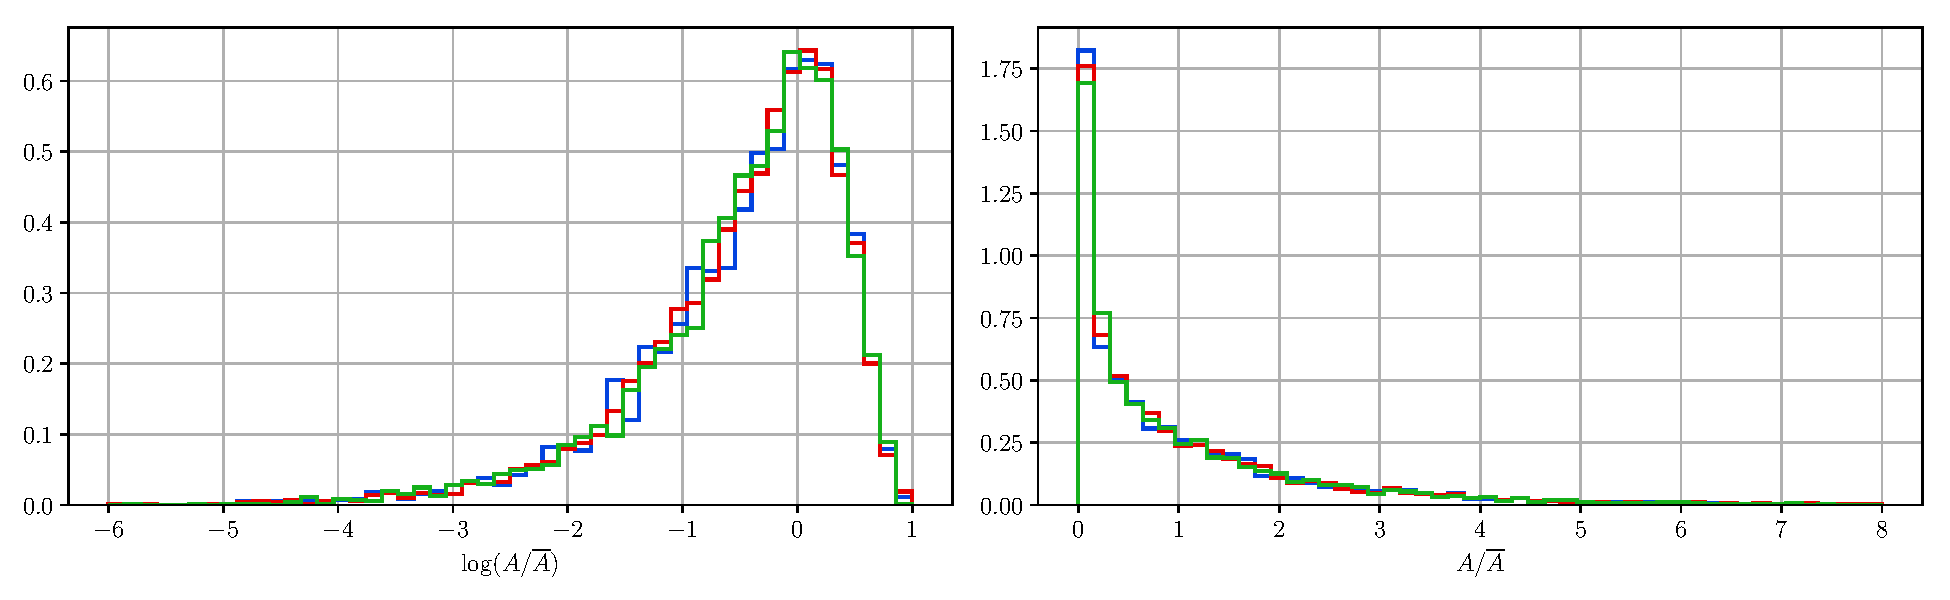
\includegraphics[scale=0.35]{figures/stored_energy/SE/areas/000070_nuclconstant_set.pdf}
    \end{figure}
    \vspace{-1em}
    First nucleations
\end{frame}

\begin{frame}{Statistics - Nucleation $\alpha = 0$ - Relative area}
\small
\centering
    \vspace{-0.5em}
    \begin{figure}
        \centering
        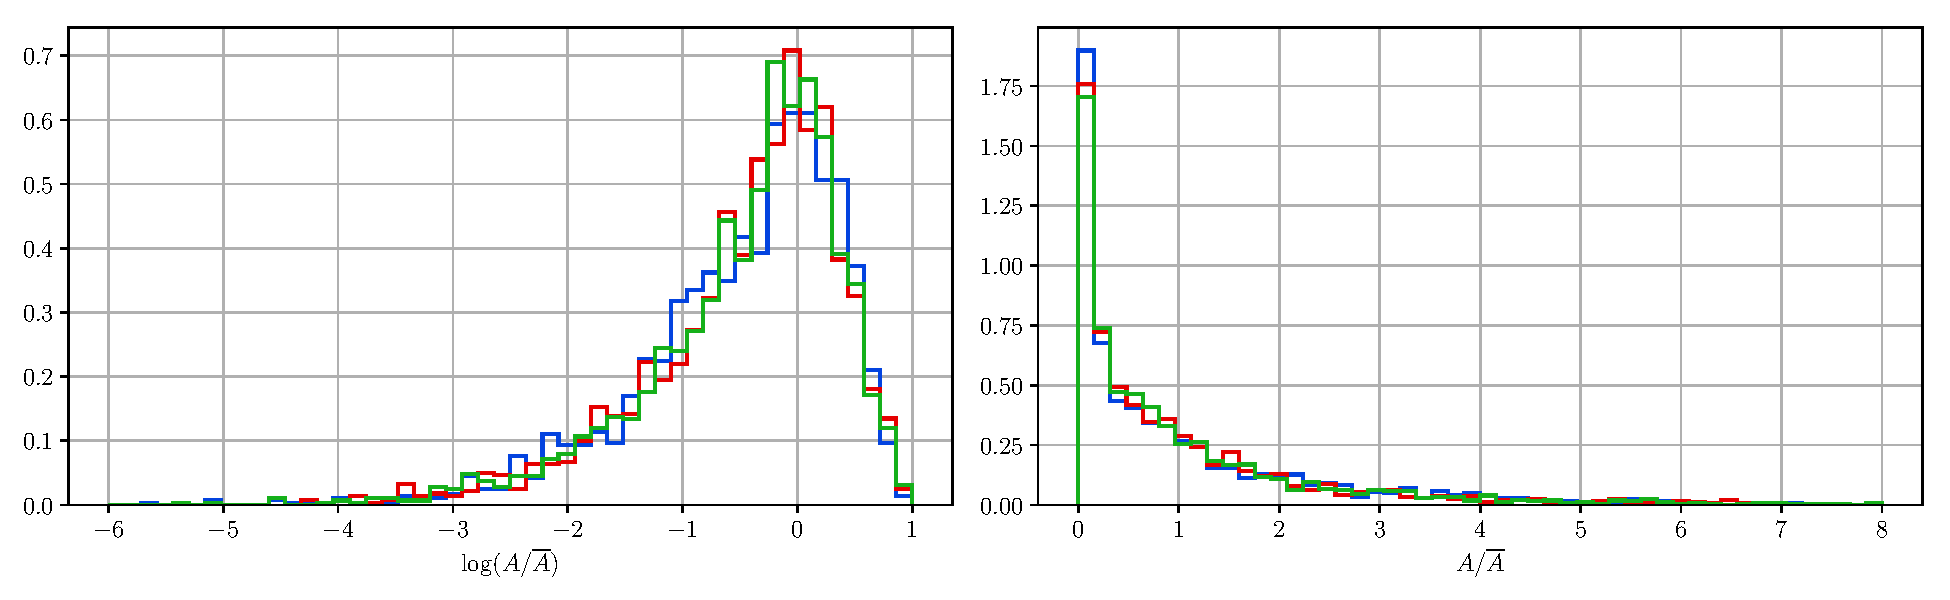
\includegraphics[scale=0.35]{figures/stored_energy/SE/areas/000110_nuclconstant_set.pdf}
    \end{figure}
    \vspace{-1em}
    Nucleation stage
    \begin{figure}
        \centering
        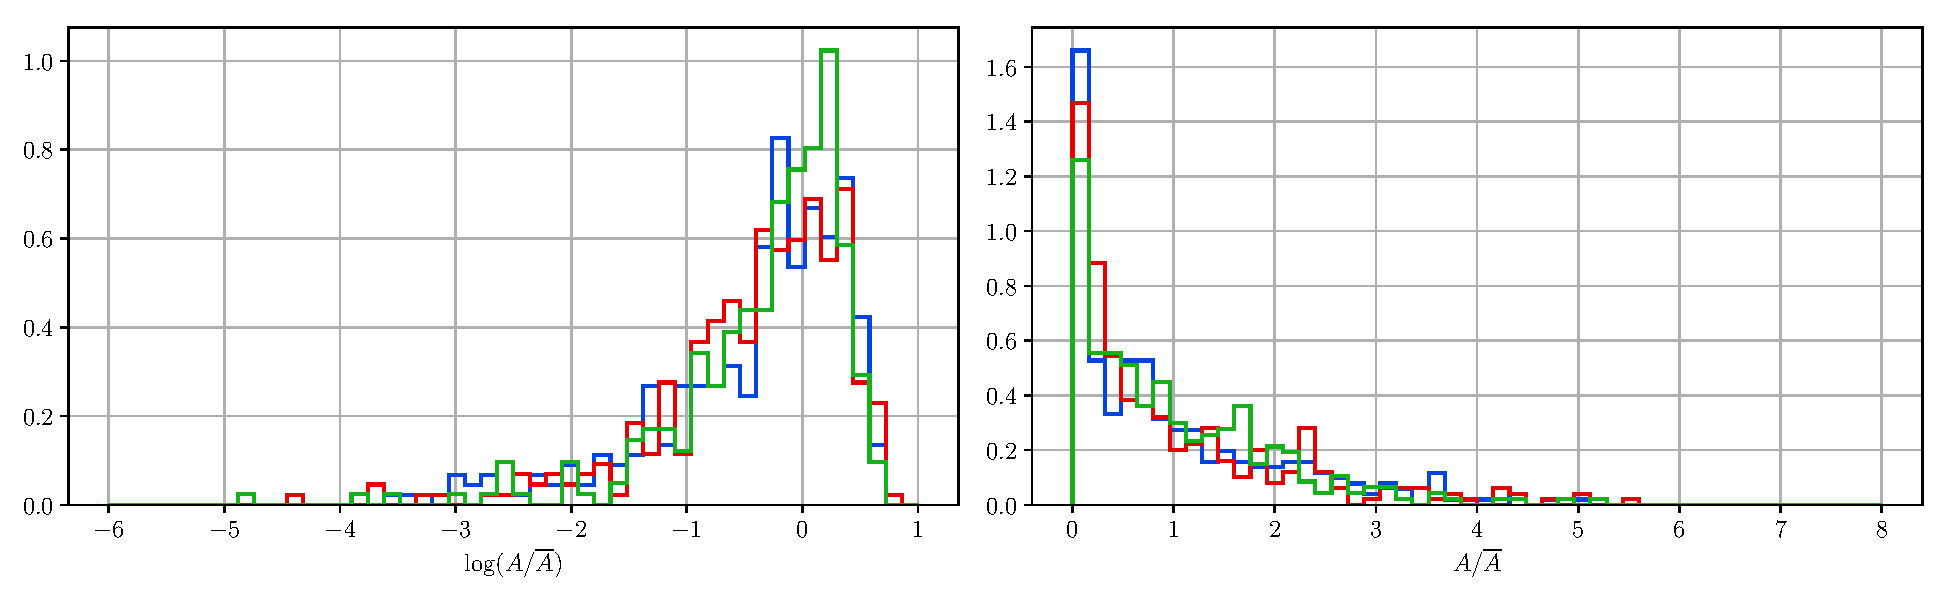
\includegraphics[scale=0.35]{figures/stored_energy/SE/areas/000240_nuclconstant_set.pdf}
    \end{figure}
    \vspace{-1em}
    Recrystallization
\end{frame}

\begin{frame}{Statistics - Nucleation $\alpha = 0$ - Dihedral angle}
    \begin{minipage}{0.5\textwidth}
    \centering
    \scriptsize
    Initial condition
    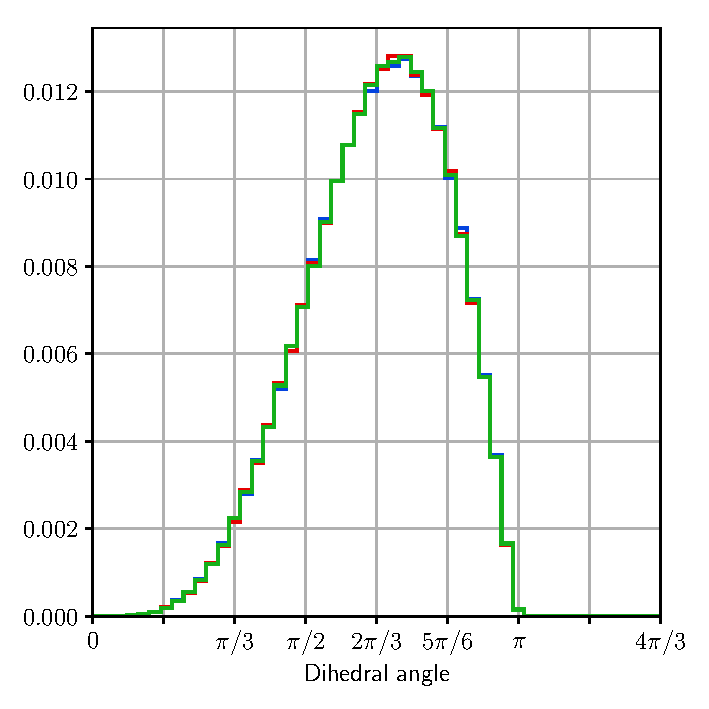
\includegraphics[trim={0 2.6em 0 1.1em},clip=true,scale=0.34]{figures/stored_energy/SE/dihedral/000000_nuclconstant_set.pdf}
    \end{minipage}%
    \begin{minipage}{0.5\textwidth}
    \centering
    \scriptsize
    First nucleations
    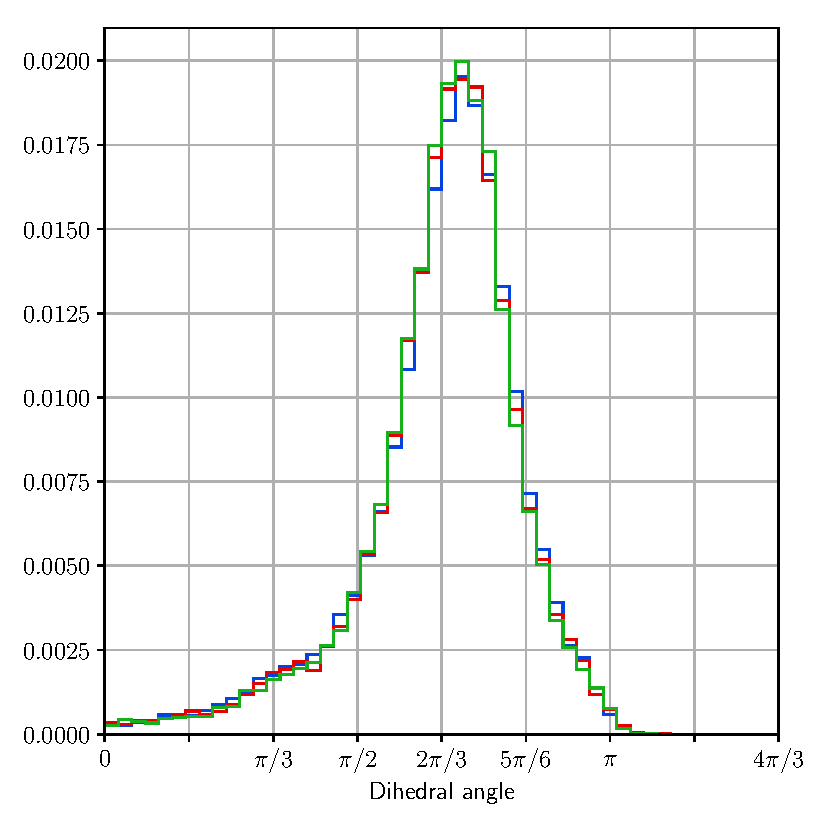
\includegraphics[trim={0 2.6em 0 1.1em},clip=true,scale=0.34]{figures/stored_energy/SE/dihedral/000070_nuclconstant_set.pdf}
    \end{minipage}\\
    \vfill
    \begin{minipage}{0.5\textwidth}
    \centering
    \scriptsize
    Nucleation stage
    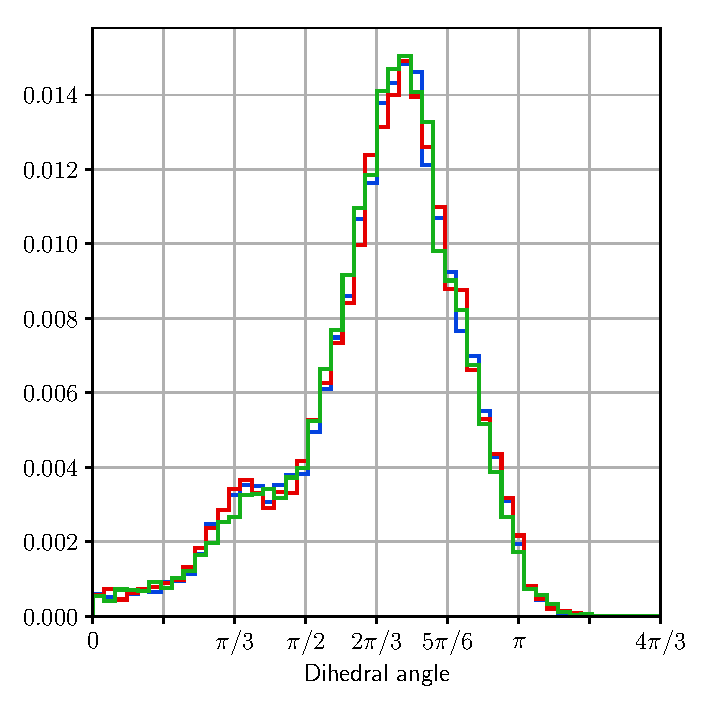
\includegraphics[trim={0 2.6em 0 1.1em},clip=true,scale=0.34]{figures/stored_energy/SE/dihedral/000110_nuclconstant_set.pdf}
    \end{minipage}%
    \begin{minipage}{0.5\textwidth}
    \centering
    \scriptsize
    Recrystallization
    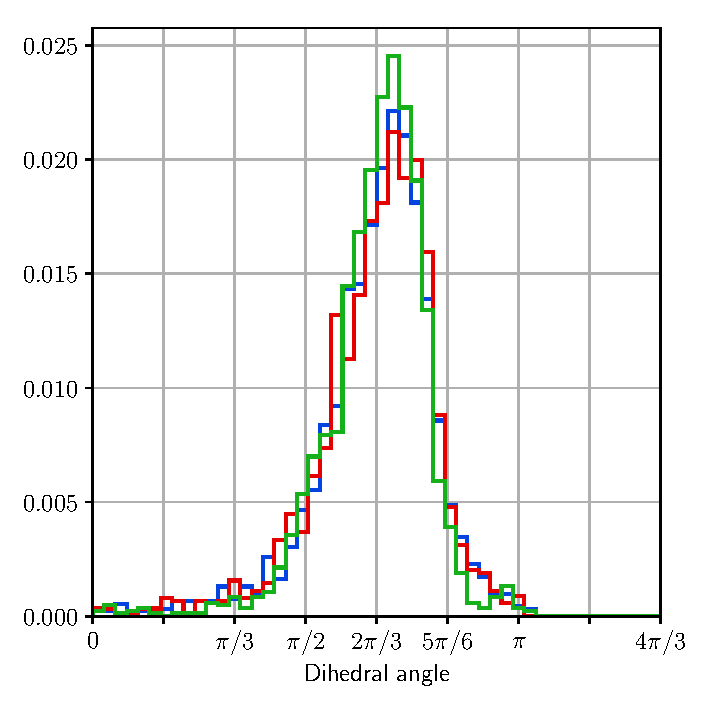
\includegraphics[trim={0 2.6em 0 1.1em},clip=true,scale=0.34]{figures/stored_energy/SE/dihedral/000240_nuclconstant_set.pdf}
    \end{minipage}
\end{frame}
\begin{frame}{Statistics - Nucleation $\alpha = 0$ - GBCD}
\small
    \begin{minipage}{\textwidth}
    \centering
    \vspace{-0.5em}
    \begin{figure}
    \centering
    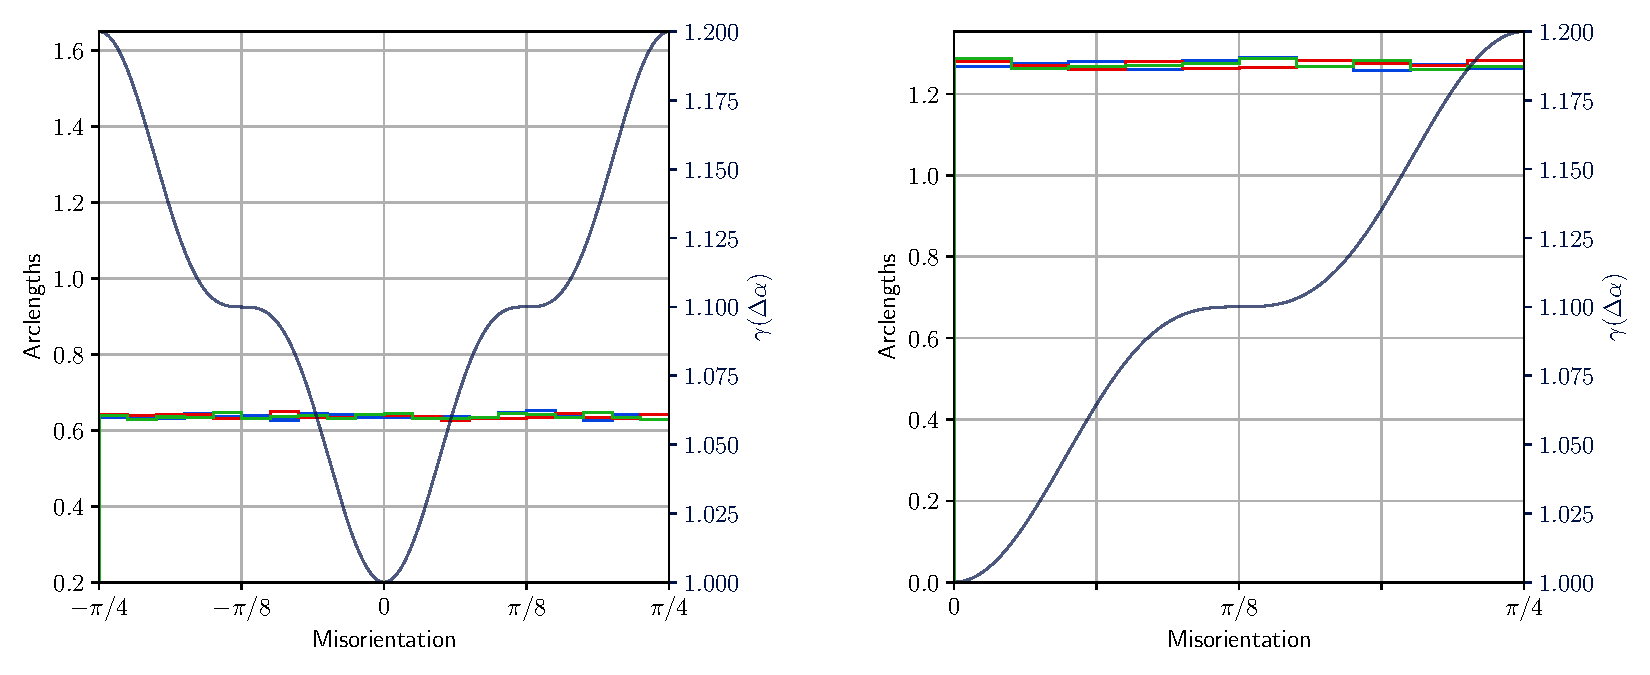
\includegraphics[scale=0.33]{figures/stored_energy/SE/gbcd/000000_nuclconstant_set.pdf}
    \end{figure}
    \vspace{-2em}
    Initial condition
    \end{minipage}\\
    \begin{minipage}{\textwidth}
    \centering
    \begin{figure}
    \centering
    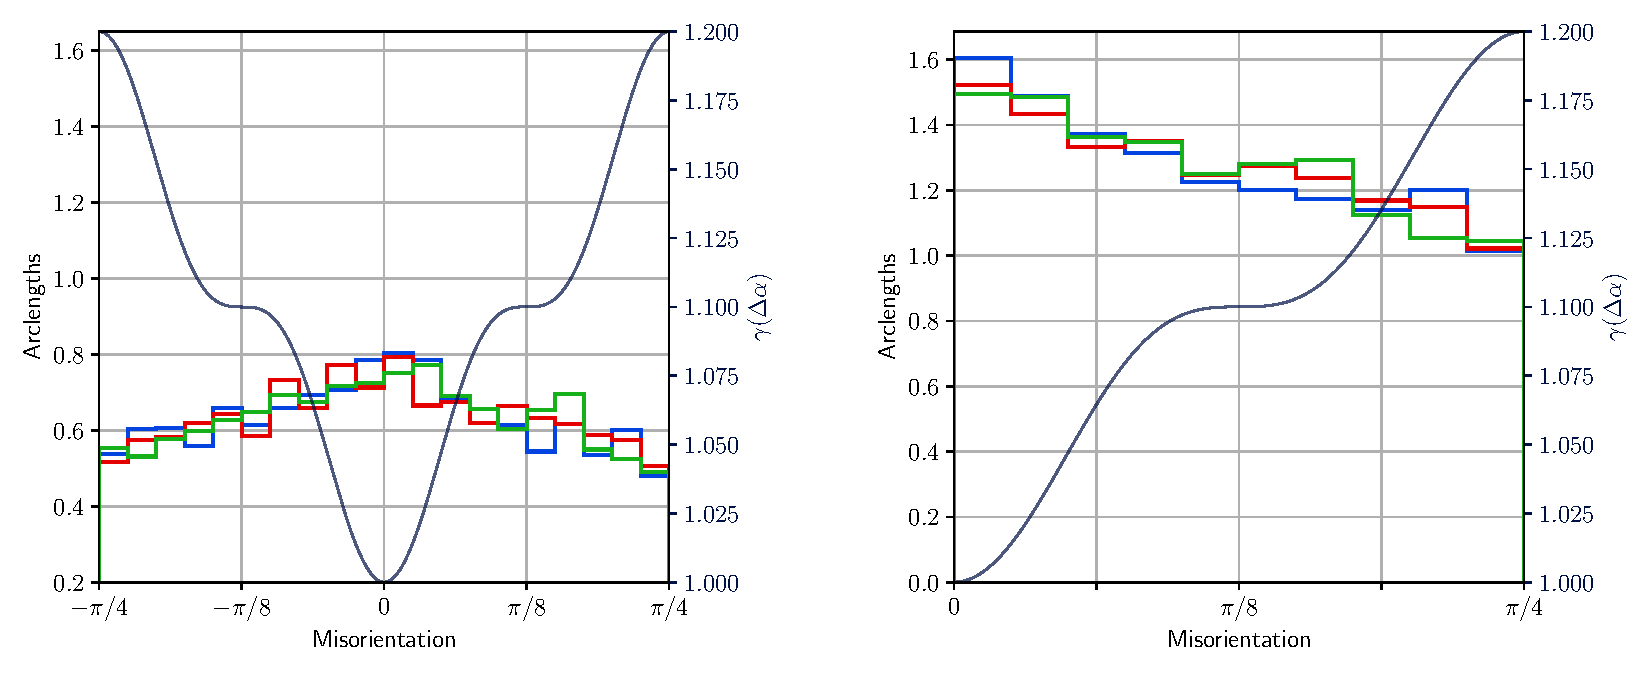
\includegraphics[scale=0.33]{figures/stored_energy/SE/gbcd/000070_nuclconstant_set.pdf}
    \end{figure}
    \vspace{-2em}
    First nucleations
    \end{minipage}
\end{frame}

\begin{frame}{Statistics - Nucleation $\alpha = 0$ - GBCD}
\small
    \begin{minipage}{\textwidth}
    \centering
    \vspace{-0.5em}
    \begin{figure}
    \centering
    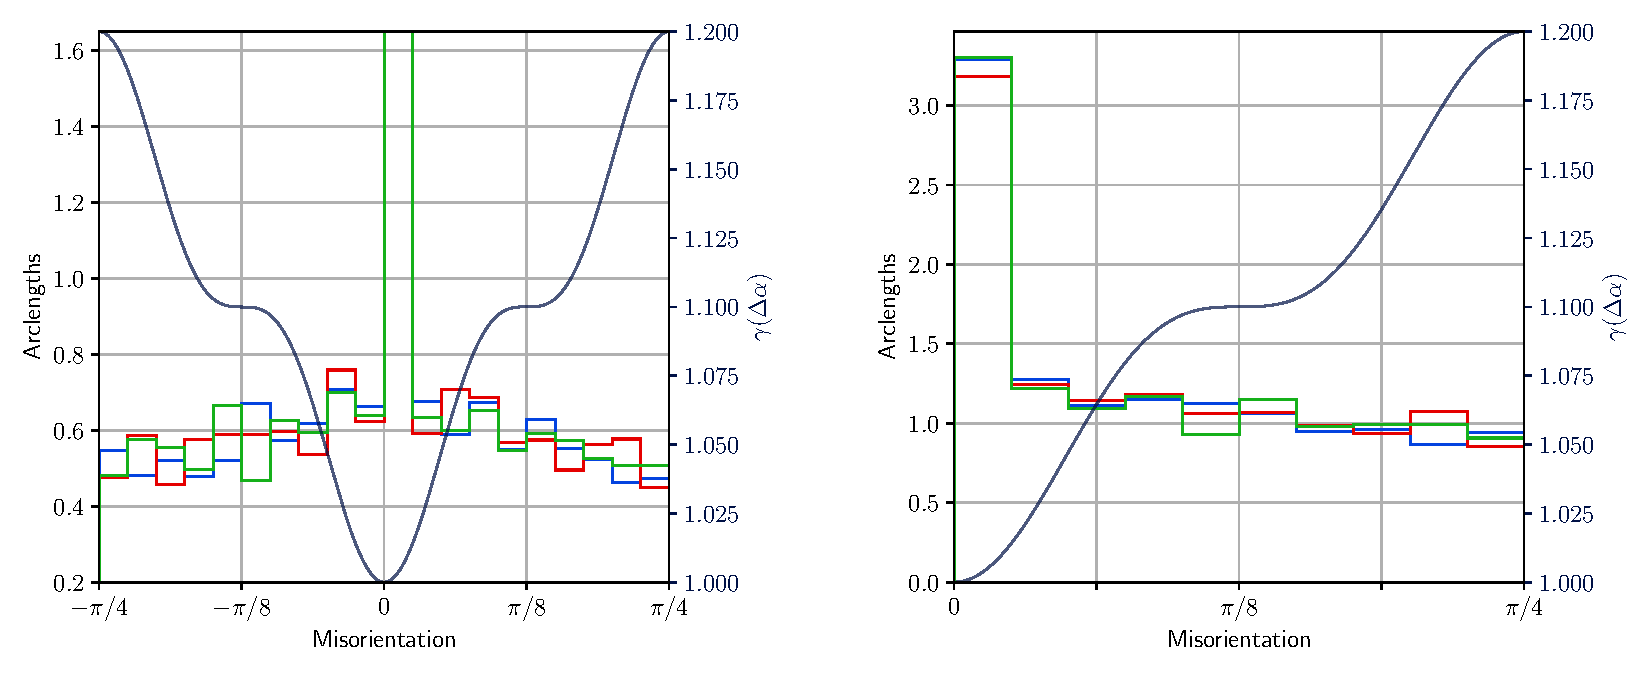
\includegraphics[scale=0.33]{figures/stored_energy/SE/gbcd/000110_nuclconstant_set.pdf}
    \end{figure}
    \vspace{-2em}
    Nucleation stage
    \end{minipage}\\
    \begin{minipage}{\textwidth}
    \centering
    \begin{figure}
    \centering
    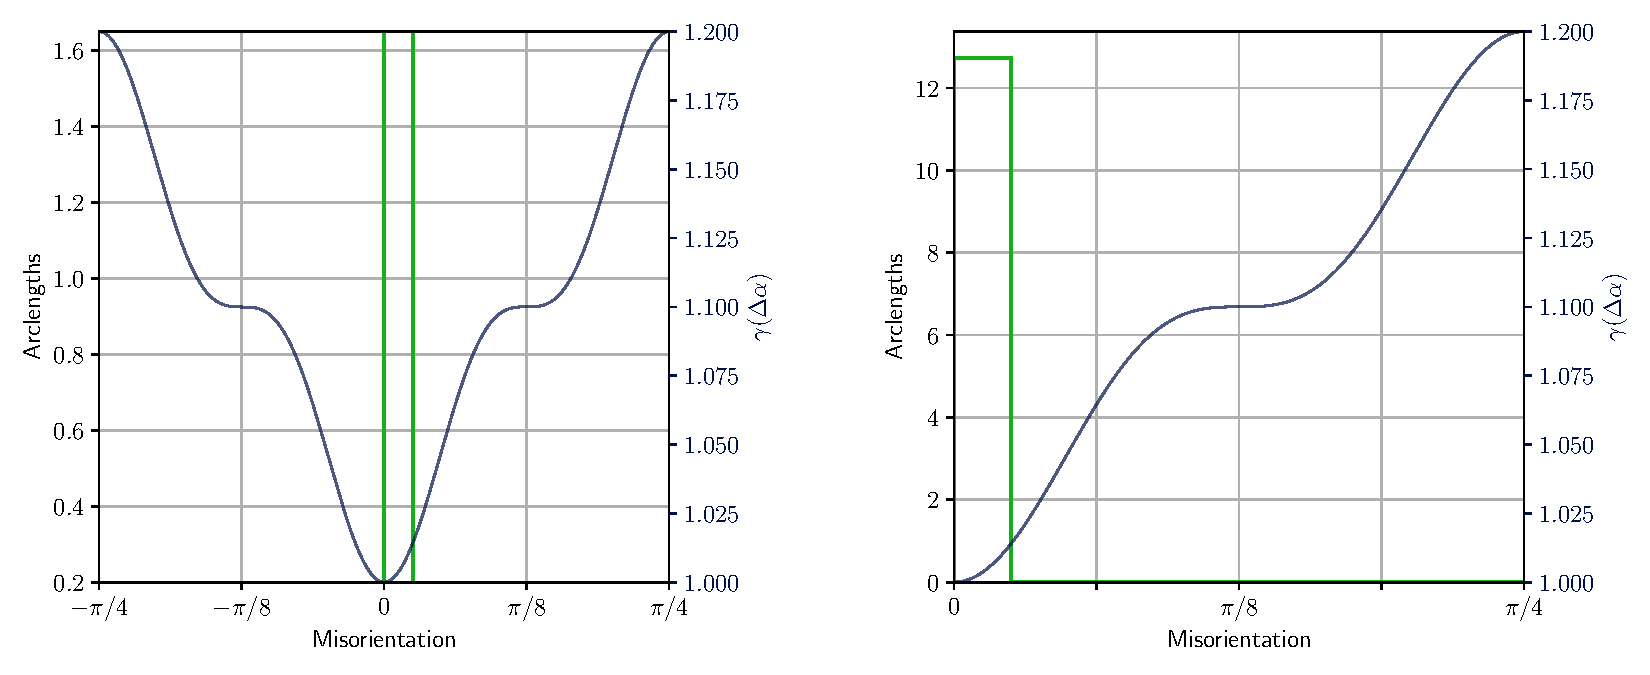
\includegraphics[scale=0.33]{figures/stored_energy/SE/gbcd/000240_nuclconstant_set.pdf}
    \end{figure}
    \vspace{-2em}
    Recrystallization
    \end{minipage}
\end{frame}

\begin{frame}{Statistics - Nucleation $\alpha = 0$ - Number of sides}
\small
    \begin{minipage}{0.5\textwidth}
    \centering
    \scriptsize
    Initial condition
    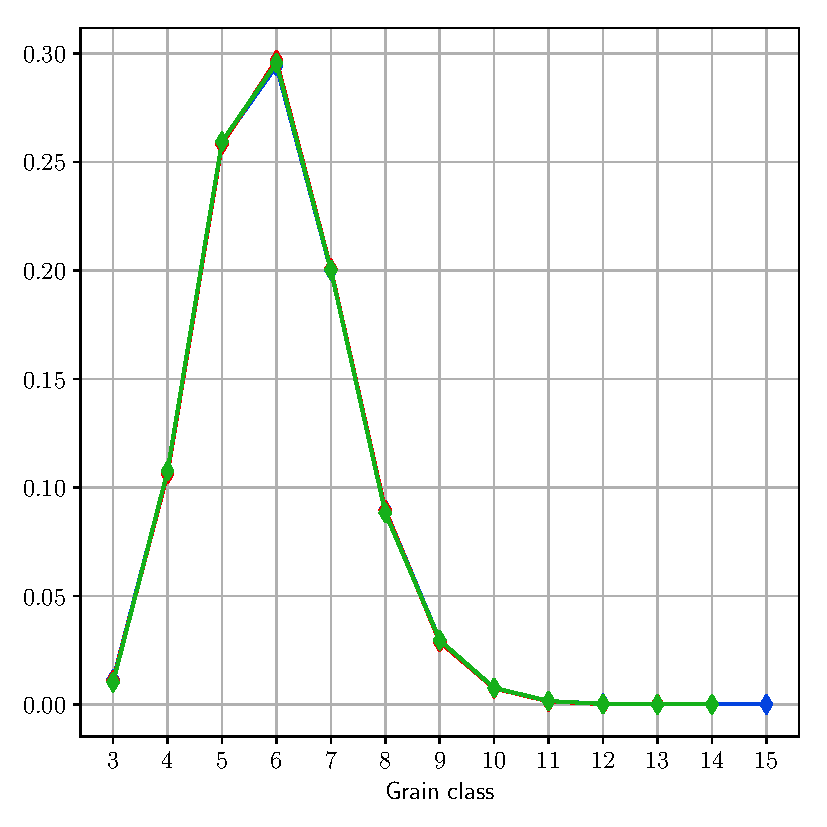
\includegraphics[trim={0 1em 0 1.1em},clip=true,scale=0.335]{figures/stored_energy/SE/nsides/000000_nuclconstant_set.pdf}
    \end{minipage}%
    \begin{minipage}{0.5\textwidth}
    \centering
    \scriptsize
    First nucleations
    \includegraphics[trim={0 1em 0 1.1em},clip=true,scale=0.335]{figures/stored_energy/SE/nsides/000070_nuclconstant_set.pdf}\\
    \end{minipage}\\
    \begin{minipage}{0.5\textwidth}
    \centering
    \scriptsize
    Nucleation Stage
    \includegraphics[trim={0 1em 0 1.1em},clip=true,scale=0.335]{figures/stored_energy/SE/nsides/000110_nuclconstant_set.pdf}
    \end{minipage}%
    \begin{minipage}{0.5\textwidth}
    \centering
    \scriptsize
    Recrystallization
    \includegraphics[trim={0 1em 0 1.1em},clip=true,scale=0.335]{figures/stored_energy/SE/nsides/000240_nuclconstant_set.pdf}
    \end{minipage}
\end{frame}
\begin{frame}{Statistics - Nucleation $\alpha = 0$  - Stored Energy distribution}
\small
    \begin{minipage}{0.5\textwidth}
    \centering
    \scriptsize
    Initial condition
    \includegraphics[trim={0 1em 0 1.1em},clip=true,scale=0.35]{figures/stored_energy/SE/se/000000_nuclconstant_set.pdf}
    \end{minipage}%
    \begin{minipage}{0.5\textwidth}
    \centering
    \scriptsize
    First nucleations
    \includegraphics[trim={0 1em 0 1.1em},clip=true,scale=0.35]{figures/stored_energy/SE/se/000070_nuclconstant_set.pdf}
    \end{minipage}\\
    \begin{minipage}{0.5\textwidth}
    \centering
    \scriptsize
    Nucleation Stage
    \includegraphics[trim={0 1em 0 1.1em},clip=true,scale=0.35]{figures/stored_energy/SE/se/000110_nuclconstant_set.pdf}
    \end{minipage}%
    \begin{minipage}{0.5\textwidth}
    \centering
    \scriptsize
    Recrystallization
    \includegraphics[trim={0 1em 0 1.1em},clip=true,scale=0.35]{figures/stored_energy/SE/se/000240_nuclconstant_set.pdf}
    \end{minipage}
\end{frame}

%%%%%% Alpha alternative

\begin{frame}{Statistics - Nucleation $\alpha$ alternative - Relative area}
\small
\centering
    \vspace{-0.5em}
    \begin{figure}
        \centering
        \includegraphics[scale=0.35]{figures/stored_energy/SE/areas/000000_nuclalternative_set.pdf}
    \end{figure}
    \vspace{-1em}
    Initial condition
    \begin{figure}
        \centering
        \includegraphics[scale=0.35]{figures/stored_energy/SE/areas/000070_nuclalternative_set.pdf}
    \end{figure}
    \vspace{-1em}
    First nucleations
\end{frame}

\begin{frame}{Statistics - Nucleation $\alpha$ alternative - Relative area}
\small
\centering
    \vspace{-0.5em}
    \begin{figure}
        \centering
        \includegraphics[scale=0.35]{figures/stored_energy/SE/areas/000110_nuclalternative_set.pdf}
    \end{figure}
    \vspace{-1em}
    Nucleation stage
    \begin{figure}
        \centering
        \includegraphics[scale=0.35]{figures/stored_energy/SE/areas/000240_nuclalternative_set.pdf}
    \end{figure}
    \vspace{-1em}
    Recrystallization
\end{frame}

\begin{frame}{Statistics - Nucleation $\alpha$ alternative - Dihedral angle}
    \begin{minipage}{0.5\textwidth}
    \centering
    \scriptsize
    Initial condition
    \includegraphics[trim={0 2.6em 0 1.1em},clip=true,scale=0.34]{figures/stored_energy/SE/dihedral/000000_nuclalternative_set.pdf}
    \end{minipage}%
    \begin{minipage}{0.5\textwidth}
    \centering
    \scriptsize
    First nucleations
    \includegraphics[trim={0 2.6em 0 1.1em},clip=true,scale=0.34]{figures/stored_energy/SE/dihedral/000070_nuclalternative_set.pdf}
    \end{minipage}\\
    \vfill
    \begin{minipage}{0.5\textwidth}
    \centering
    \scriptsize
    Nucleation stage
    \includegraphics[trim={0 2.6em 0 1.1em},clip=true,scale=0.34]{figures/stored_energy/SE/dihedral/000110_nuclalternative_set.pdf}
    \end{minipage}%
    \begin{minipage}{0.5\textwidth}
    \centering
    \scriptsize
    Recrystallization
    \includegraphics[trim={0 2.6em 0 1.1em},clip=true,scale=0.34]{figures/stored_energy/SE/dihedral/000240_nuclalternative_set.pdf}
    \end{minipage}
\end{frame}

\begin{frame}{Statistics - Nucleation $\alpha$ alternative - GBCD}
\small
    \begin{minipage}{\textwidth}
    \centering
    \vspace{-0.5em}
    \begin{figure}
    \centering
    \includegraphics[scale=0.33]{figures/stored_energy/SE/gbcd/000000_nuclalternative_set.pdf}
    \end{figure}
    \vspace{-2em}
    Initial condition
    \end{minipage}\\
    \begin{minipage}{\textwidth}
    \centering
    \begin{figure}
    \centering
    \includegraphics[scale=0.33]{figures/stored_energy/SE/gbcd/000070_nuclalternative_set.pdf}
    \end{figure}
    \vspace{-2em}
    First nucleations
    \end{minipage}
\end{frame}

\begin{frame}{Statistics - Nucleation $\alpha$ alternative - GBCD}
\small
    \begin{minipage}{\textwidth}
    \centering
    \vspace{-0.5em}
    \begin{figure}
    \centering
    \includegraphics[scale=0.33]{figures/stored_energy/SE/gbcd/000110_nuclalternative_set.pdf}
    \end{figure}
    \vspace{-2em}
    Nucleation stage
    \end{minipage}\\
    \begin{minipage}{\textwidth}
    \centering
    \begin{figure}
    \centering
    \includegraphics[scale=0.33]{figures/stored_energy/SE/gbcd/000240_nuclalternative_set.pdf}
    \end{figure}
    \vspace{-2em}
    Recrystallization
    \end{minipage}
\end{frame}

\begin{frame}{Statistics - Nucleation $\alpha$ alternative - Number of sides}
\small
    \begin{minipage}{0.5\textwidth}
    \centering
    \scriptsize
    Initial condition
    \includegraphics[trim={0 1em 0 1.1em},clip=true,scale=0.335]{figures/stored_energy/SE/nsides/000000_nuclalternative_set.pdf}
    \end{minipage}%
    \begin{minipage}{0.5\textwidth}
    \centering
    \scriptsize
    First nucleations
    \includegraphics[trim={0 1em 0 1.1em},clip=true,scale=0.335]{figures/stored_energy/SE/nsides/000070_nuclalternative_set.pdf}\\
    \end{minipage}\\
    \begin{minipage}{0.5\textwidth}
    \centering
    \scriptsize
    Nucleation Stage
    \includegraphics[trim={0 1em 0 1.1em},clip=true,scale=0.335]{figures/stored_energy/SE/nsides/000110_nuclalternative_set.pdf}
    \end{minipage}%
    \begin{minipage}{0.5\textwidth}
    \centering
    \scriptsize
    Recrystallization
    \includegraphics[trim={0 1em 0 1.1em},clip=true,scale=0.335]{figures/stored_energy/SE/nsides/000240_nuclalternative_set.pdf}
    \end{minipage}
\end{frame}

% \begin{frame}{Statistics - Nucleation $\alpha$ alternative}
% \small
%     \begin{minipage}{0.5\textwidth}
%     \centering
%     \includegraphics[scale=0.35]{figures/stored_energy/SE/nsides/000110_nuclalternative_set.pdf}\\
%     Nucleation Stage
%     \end{minipage}%
%     \begin{minipage}{0.5\textwidth}
%     \centering
%     \includegraphics[scale=0.35]{figures/stored_energy/SE/nsides/000240_nuclalternative_set.pdf}\\
%     Recrystallization
%     \end{minipage}
% \end{frame}

\begin{frame}{Statistics - Nucleation $\alpha$ alternative - Stored Energy distribution}
\small
    \begin{minipage}{0.5\textwidth}
    \centering
    \scriptsize
    Initial condition
    \includegraphics[trim={0 1em 0 1.1em},clip=true,scale=0.35]{figures/stored_energy/SE/se/000000_nuclalternative_set.pdf}
    \end{minipage}%
    \begin{minipage}{0.5\textwidth}
    \centering
    \scriptsize
    First nucleations
    \includegraphics[trim={0 1em 0 1.1em},clip=true,scale=0.35]{figures/stored_energy/SE/se/000070_nuclalternative_set.pdf}
    \end{minipage}\\
    \begin{minipage}{0.5\textwidth}
    \centering
    \scriptsize
    Nucleation Stage
    \includegraphics[trim={0 1em 0 1.1em},clip=true,scale=0.35]{figures/stored_energy/SE/se/000110_nuclalternative_set.pdf}
    \end{minipage}%
    \begin{minipage}{0.5\textwidth}
    \centering
    \scriptsize
    Recrystallization
    \includegraphics[trim={0 1em 0 1.1em},clip=true,scale=0.35]{figures/stored_energy/SE/se/000240_nuclalternative_set.pdf}
    \end{minipage}
\end{frame}

% \begin{frame}{Statistics - Nucleation $\alpha$ alternative}
% \small
%     \begin{minipage}{0.5\textwidth}
%     \centering
%     \includegraphics[scale=0.4]{figures/stored_energy/SE/se/000110_nuclalternative_set.pdf}\\
%     Nucleation Stage
%     \end{minipage}%
%     \begin{minipage}{0.5\textwidth}
%     \centering
%     \includegraphics[scale=0.4]{figures/stored_energy/SE/se/000240_nuclalternative_set.pdf}\\
%     Recrystallization
%     \end{minipage}
% \end{frame}


\section[3D Implicit-transition Model]{The Implicit-transition Model for 3D Grain Growth}
\begin{frame}{The Implicit-transition Model}
    This model is inspired in the Vertex Model~\cite{torres2015}. We have {\color{MidnightBlue}flat boundaries} (polyhedra faces) instead of 2D curves. The point where three boundaries meet is called a {\color{Red}triple line}, and four boundaries meet at {\color{mygreen}quadruple junctions}.
    %
    \begin{figure}
        \centering
        \includegraphics[scale=0.6]{figures/extras/3dscheme.pdf}
    \end{figure}
    %
\end{frame}
\begin{frame}{The Implicit-transition Model}
    Voronoi tessellation has been traditionally used for initial conditions of grain growth~\cite{Barmak2013,BarralesMora2008,Kinderlehrer2006,Lazar2011,Syha2010,torres2015}. Given a \textbf{generator points} set $\mathcal{P}$ for Voronoi:
    \begin{equation*}
    \mathcal{P} = \mathcal{P}(t) = \{ \mathbf{P}^{(1)}, \mathbf{P}^{(2)}, \dotsc, \mathbf{P}^{(N)} \}.
    \end{equation*}
    \vspace{-1em}
    \begin{figure}
        \centering
        \includegraphics[trim={0 3em 0 2em},clip=true,scale=0.37]{figures/extras/2dschemewithcenters.pdf}
    \end{figure}
    \vspace{-0.5em}
    We can move generator points and tessellate to obtain a new grain structure performing topological transitions \emph{implicitly}. This continuous motion is stable in front of small changes~\cite{reem2011geometric}.
\end{frame}

\begin{frame}{The Implicit-transition Model}
    Why \emph{implicit}? Topological transitions in 3D become more difficult to handle.
    \begin{figure}
        \centering
        \includegraphics[scale=0.25]{figures/extras/3dflipping.png}
    \end{figure}
    2D transitions are difficult enough to implement and detect. In 3D the complexity increases since we are flipping surfaces~\cite{BarralesMora2008}
\end{frame}


\begin{frame}{The Implicit-transition Model}
    The total energy accounts grain boundary energies over surfaces:
    \begin{equation*}
        E = \sum_{k=1}^{K} \int_{\bnd^{(k)}} \sigma_k\,dA.
    \end{equation*}
We aim to minimize this quantity and we propose the following evolution equation for generator points based on the tangent vectors along triple lines connecting the grain $\grn$ with its neighbors:
\begin{equation*}
    \dot{\mathbf{P}}^{(\grn)} = \sum_{m=1}^{M} \gamma^{(m,l)}\mathbf{T}^{(m,l)},
\end{equation*}
where $\gamma$ is an energy term related to a triple line and $\T$ is a unit tangent along the triple lines connected to other grains. This proposal is not derivated from $E$ but aims to minimize energy.\\
\end{frame}

\begin{frame}{The Implicit-transition Model}
\begin{figure}
    \centering
    \includegraphics[scale=0.25]{figures/extras/views.png}
    \caption{Front and back views of a \textcolor{blue}{grain} with neighbors and \textcolor{red}{triple lines} from where tangents are computed. Colored grains are marked for spatial reference.}
\end{figure}
This model was published and presented at the 36th International Conference of the Chilean Computer Science Society~\cite{sazo2017implicit}
\end{frame}

\subsection{Numerical Experiments}

\begin{frame}
   \centering
   \movie[width=\textwidth,height=\textheight]{3D grain}{/home/asazo/Escritorio/3d_single_grain.mp4}
\end{frame}

\begin{frame}
   \centering
   \movie[width=\textwidth,height=\textheight]{Simulation idea}{/home/asazo/Escritorio/normals.mov}
\end{frame}

\begin{frame}{Energy Minimization}
    This model decreases the total energy of the system \emph{asymptotically} but not \emph{monotonically}.
    \begin{figure}
        \centering
        \includegraphics[scale=0.5]
        {figures/3d_voronoi/3D_energy.pdf}
    \end{figure}
\end{frame}

\begin{frame}{Topological Transitions}
We were able to recover flippings, grain removals and surface removals.
\vspace{-0.2em}
\begin{figure}
    \centering
    \includegraphics[scale=0.2]{figures/3d_voronoi/3D_flipping.pdf}\\
    \includegraphics[scale=0.2]{figures/3d_voronoi/3D_surface_removal.pdf}\\
    \includegraphics[scale=0.2]{figures/3d_voronoi/3D_grain_removal.pdf}
\end{figure}
\end{frame}

\section{Conclusions}
\begin{frame}{Conclusions}
\begin{itemize}
    \item We studied 2D and 3D models of grain growth and nucleation via mathematical modeling and analysis, numerical computations and statistics.
    \item Improvement of the Coupled Model to capture \textbf{curvature-based motion} and correction of interior points along the boundaries via an orthogonal \textbf{tangential component}. Also we improved flipping detection via \textbf{Multi-Step methods}, \textbf{improved interval for $t_{\text{ext}}$} and the \textbf{Predictor-Corrector Algorithm}.
    \item Variation of $\mu$ and $\lambda$ mobilities allow us to recover statistics from dihedral angle at $2\pi/3$, number of sides distribution as in vertex model and curvature model and the Von Neumann-Mullins $(n-6)$ rule.
\end{itemize}
\end{frame}

\begin{frame}{Conclusions}
    \begin{itemize}
        \item An extended Continuous Vertex Model with Nucleation was developed.
        \item We analyzed the effect of Stored Energy $\SE$ over triple junctions evolution. We found that \textbf{there is a limit on $\SE$ values} where grains can grow stable.
        \item Study of \textbf{how to nucleate} at triple junctions and the \textbf{size of nucleation} $r_c$ required to grow. This leads to a temporal increase in the total energy but we still minimize it.
        \item We found an interesting behavior of the total energy of the system when choosing different orientation criteria.
        \item Stages of grain growth and nucleation can be identified clearly. We recover the GBCD in the case of $\alpha$ alternative.
    \end{itemize}
\end{frame}

\begin{frame}{Conclusions}
    \begin{itemize}
        \item We developed the \textbf{parallel polling system} for handling topological transitions in parallel to support the native implementation of the Coupled Model and the Stored Energy Vertex Model in GPU.
        \item The \textbf{Implicit-transition Model} based on 2D Vertex Model was presented. This model handles implicitly topological transitions by generating the grain network at each iteration via Voronoi tessellation. We effectively decrease the energy asymptotically but not monotonically.
        \item We analyzed a 3D model and we obtained via image analysis techniques 2D slices and then we were able to extract the relative area distribution.
    \end{itemize}
\end{frame}

\begin{frame}{Future Work}
    
\end{frame}

\begin{frame}
     \centering
   \movie[width=\textwidth,height=\textheight]{Simulation}{/home/asazo/Escritorio/All_4.mp4}
\end{frame}

% All of the following is optional and typically not needed.
\appendix
\begin{frame}[allowframebreaks]
    \frametitle{References}
    \bibliographystyle{ieeetr}
    %\bibliographystyle{alpha}
    \bibliography{references.bib}
\end{frame}

%%%% Appendix %%%%


%%% Closed boundary motion  %%%
\section{Closed Boundary Motion}
\begin{frame}{Closed Boundary Motion}
Let $\vxi(s,t) = \langle x(s,t), y(s,t) \rangle,\, s \in [0, 2\pi]$, $t >  0$ a closed curve in $\mathbb{R}^2$, \ie $\vxi(0, t) = \vxi(2\pi,t)$. This will be our \emph{closed boundary}. The total energy of this boundary is:
\begin{equation*}
    E(t) = \int_0^{2\pi} \norm{\mylvec(s,t)} ds.
\end{equation*}
Taking the derivative of $E$ with respect to time we obtain:
\begin{align*}
    \frac{dE}{dt} &= \int_0^{2\pi} \frac{\mylvec(s,t)}{\norm{\mylvec(s,t)}}\cdot \frac{\partial \mylvec}{\partial s}(s,t)\,ds\\
    &= -\int_0^{2\pi} \frac{\partial \T}{\partial s}(s,t)\cdot \vel(s,t)\, ds.
\end{align*}
We will use this equation to understand the motion of a closed boundary.
\end{frame}

\subsection{Curvature Based Motion}
\begin{frame}{Curvature Based Motion}
Assuming that the velocity of the boundary is in the direction of the normal vector $\N$ and proportional to its curvature $\kappa(s,t)$~\cite{Kinderlehrer2006}, we define the boundary velocity as:
\begin{equation*}
    \vel(s,t) = \kappa(s,t)\N(s,t).
\end{equation*}
If we take the derivative of $\T$ with respect to the boundary arc length $\AL$ we obtain:
\begin{align}
    \frac{\partial \T}{\partial \AL} &= \kappa(s,t)\N(s,t) \nonumber\\
    \frac{\partial \T}{\partial s}(s,t) \frac{ds}{d\AL}&= \kappa(s,t)\N(s,t)
    \label{eq:dTds_dsdAL}
\end{align}
Notice the term $ds/d\AL$. The definition of the arc length up to a parameter $s$ is:
\begin{equation*}
    \AL(s) = \int_0^s \norm{\mylvec(s,t)}\, ds.
\end{equation*}
\end{frame}

\begin{frame}{Curvature Based Motion}
\begin{equation*}
    \frac{d\AL}{ds} = \norm{\mylvec(s,t)}\quad \Rightarrow  \quad \frac{ds}{d\AL} = \frac{1}{\norm{\mylvec(s,t)}}.
\end{equation*}
Replacing this result in \eqref{eq:dTds_dsdAL} we obtain:
\begin{equation*}
    \frac{1}{\norm{\mylvec(s,t)}} \frac{\partial \T}{\partial s}(s,t) = \kappa(s,t)\N(s,t).
\end{equation*}
Finally we define the boundary velocity in terms of the derivative of the tangent vector $\T$ as
\begin{equation*}
    \vel(s,t) = \frac{1}{\norm{\mylvec(s,t)}} \frac{\partial \T}{\partial s}(s,t).
\end{equation*}
\end{frame}

\subsection{Motion with Discrete Points}
\begin{frame}{Motion with Discrete Points}
Consider the collocation points $\vertices = \{\x_1, \ldots, \x_n\}$ and an interpolating function $\phi(s)$. The closed boundary can be represented as:
\begin{equation*}
    \vxi(s,t) = \sum_{i=1}^n \x_i(t) \phi_i(s).
\end{equation*}
where $\phi(s)$ can be the $\sinc(s)$ periodic function. Therefore its velocity is:
\begin{equation*}
    \vel(s,t) = \sum_{i=1}^n \dotx_i(t) \phi_i(s).
\end{equation*}
\end{frame}

\subsection{Numerical Experiments}
\begin{frame}{Circular Boundary Motion}
    \begin{figure}
        \centering
        \includegraphics[trim={0 0 0 6em}, clip=true, scale=0.43]{figures/closed_boundary/circularboundary.pdf}
    \end{figure}
\end{frame}

\begin{frame}{Circular Boundary Area}
    \begin{figure}
        \centering
        \includegraphics[trim={0 0 0 0}, clip=true, scale=0.43]{figures/closed_boundary/circularboundary_area.pdf}
    \end{figure}
\end{frame}

\begin{frame}{Circular Boundary Energy}
     \begin{figure}
        \centering
        \includegraphics[trim={0 0 0 0}, clip=true, scale=0.43]{figures/closed_boundary/circularboundary_energy.pdf}
    \end{figure}
\end{frame}

\begin{frame}{Non-regular Boundary Motion}
     \begin{figure}
        \centering
        \includegraphics[trim={0 0 0 6em}, clip=true, scale=0.43]{figures/closed_boundary/nonregularboundary.pdf}
    \end{figure}
\end{frame}

\begin{frame}{Non-regular Boundary Area}
     \begin{figure}
        \centering
        \includegraphics[trim={0 0 0 0}, clip=true, scale=0.43]{figures/closed_boundary/nonregularboundary_area.pdf}
    \end{figure}
\end{frame}

\begin{frame}{Non-regular Boundary Energy}
     \begin{figure}
        \centering
        \includegraphics[trim={0 0 0 0}, clip=true, scale=0.43]{figures/closed_boundary/nonregularboundary_energy.pdf}
    \end{figure}
\end{frame}

\section{The Parallel Polling System}

\subsection{Sequential Management}
\begin{frame}{Sequential Management}
\begin{itemize}
    \item The Coupled Model and the Stored Energy Vertex Model (SEVM) depends of the structure of vertices and boundaries.
    \item Flippings can be detected by sorting the boundary set $\boundaries$ by $t_{\text{ext}}$ in decreasing order.
    \item We can iteratively decide the safe flippings by labeling the vertices related to each boundary until we find that a boundary has a repeated labeled vertex.
\end{itemize}
\end{frame}

\begin{frame}
\begin{algorithmic}[1]
\Procedure{SEQUENTIAL}{}
\State $\boundaries \gets$ Clear flip and inhibited state for each boundary
\State $\boundaries \gets$ Update $t_{\text{ext}}$ for each boundary
\State $\boundaries_{\text{flip}} \gets$ Boundaries to flip with $t_{\text{ext}} \in [0, \Delta t]$ 
\State $\boundaries_{\text{flip}} \gets$ Sort boundaries by $t_{\text{ext}}$ in decreasing order
\State $\boundaries_{\text{tmp}} \gets \varnothing,\quad$ Empty list of boundaries visited
\State $\vertices_{\text{tmp}} \gets \varnothing,\quad$ Empty list of vertices visited
\ForEach{$\Gamma \in \boundaries_{\text{flip}}$}
    \State $\{\x_i, \x_j\} \gets $ Vertices of $\Gamma$
    \If{$ \vertices_{\text{tmp}} \cap \{\x_i, \x_j\} = \varnothing$}
        \State $\boundaries_{\text{tmp}} \gets \boundaries_{\text{tmp}} \cup \Gamma$
        \State $\vertices_{\text{tmp}} \gets \vertices_{\text{tmp}} \cup \{\x_i, \x_j\}$
    \Else
        \State \Return $\boundaries_{\text{tmp}}$
    \EndIf
\EndFor
\EndProcedure
\end{algorithmic}
\end{frame}

\begin{frame}{Sequential Management}
\begin{itemize}
    \item We need more significant statistics. Hundreds of thousands of grains must be simulated.
    \item A parallel approach in CPU still can handle topological transitions with the mentioned algorithm, but might not scale with the number of grains.
    \item Since the implementation of the Coupled Model and SEVM  is done in GPU, it would be helpful to develop a parallel algorithm for solving the transitions.
\end{itemize}
\end{frame}

\subsection{Parallel Management}
\begin{frame}{Parallel Management}
\begin{itemize}
    \item The parallel management is based in the idea of treating each basic \emph{unit}  (boundaries, vertices) by separate, performing operations in parallel related to managing their own states,
    \item We compute $t_\text{ext}$ for each boundary. Each vertex first \emph{votes} for their boundary with lowest $t_\text{ext}$ . Then each boundary \emph{counts} the received votes. Boundaries with two votes can flip and block neighbor boundaries for flipping (\ie they cannot be voted).
    \item This procedure is iterated until we converge and we cannot vote anymore.
\end{itemize}
\end{frame}

\begin{frame}{Parallel Management}
    \begin{figure}[t]
    \centering
    \subfloat[] {    
    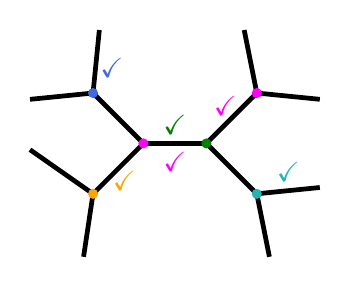
\begin{tikzpicture}[scale=0.8]
    % Boundaries
    \draw[line width=0.6mm, black] (0,0) -- (1,0);
    %
    \draw[line width=0.6mm, black] (0,0) -- (-0.8,0.8);
    \draw[line width=0.6mm, black] (-0.8,0.8) -- (-0.7, 1.8);
    \draw[line width=0.6mm, black] (-0.8,0.8) -- (-1.8,0.7);
    %
    \draw[line width=0.6mm, black] (0,0) -- (-0.8,-0.8);
    \draw[line width=0.6mm, black] (-0.8,-0.8) -- (-1.8, -0.1);
    \draw[line width=0.6mm, black] (-0.8,-0.8) -- (-0.95, -1.8);
    %
    \draw[line width=0.6mm, black] (1,0) -- (1.8,0.8);
    \draw[line width=0.6mm, black] (1.8,0.8) -- (1.6, 1.8);
    \draw[line width=0.6mm, black] (1.8,0.8) -- (2.8,0.7);
    %
    \draw[line width=0.6mm, black] (1,0) -- (1.8,-0.8);
    \draw[line width=0.6mm, black] (1.8,-0.8) -- (2, -1.8);
    \draw[line width=0.6mm, black] (1.8,-0.8) -- (2.8,-0.7);
    % Vertices
    \filldraw [Magenta] (0,0) circle (2pt);
    \filldraw [RoyalBlue] (-0.8,0.8) circle (2pt);
    \filldraw [Orange] (-0.8,-0.8) circle (2pt);
    \filldraw [Green] (1,0) circle (2pt);
    \filldraw [Fuchsia] (1.8,0.8) circle (2pt);
    \filldraw [TealBlue] (1.8,-0.8) circle (2pt);
    % Votes
    \node[draw=none, color=Magenta] at (0.5, -0.3) {$\checkmark$};
    \node[draw=none, color=RoyalBlue] at (-0.5, 1.2) {$\checkmark$};
    \node[draw=none, color=Orange] at (-0.3, -0.6) {$\checkmark$};
    \node[draw=none, color=Green] at (0.5, 0.3) {$\checkmark$};
    \node[draw=none, color=Fuchsia] at (1.3, 0.6) {$\checkmark$};
    \node[draw=none, color=TealBlue] at (2.3, -0.45) {$\checkmark$};
    %%
    \end{tikzpicture}
    \label{fig:poll1}
    }\hspace{5em}
    \subfloat[] {    
    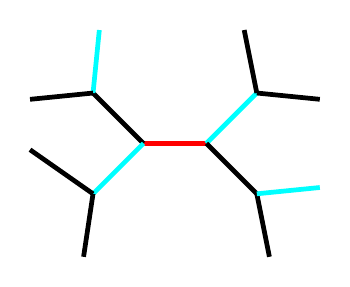
\begin{tikzpicture}[scale=0.8]
    % Boundaries
    \draw[line width=0.6mm, red] (0,0) -- (1,0);
    %
    \draw[line width=0.6mm, black] (0,0) -- (-0.8,0.8);
    \draw[line width=0.6mm, Cyan] (-0.8,0.8) -- (-0.7, 1.8);
    \draw[line width=0.6mm, black] (-0.8,0.8) -- (-1.8,0.7);
    %
    \draw[line width=0.6mm, Cyan] (0,0) -- (-0.8,-0.8);
    \draw[line width=0.6mm, black] (-0.8,-0.8) -- (-1.8, -0.1);
    \draw[line width=0.6mm, black] (-0.8,-0.8) -- (-0.95, -1.8);
    %
    \draw[line width=0.6mm, Cyan] (1,0) -- (1.8,0.8);
    \draw[line width=0.6mm, black] (1.8,0.8) -- (1.6, 1.8);
    \draw[line width=0.6mm, black] (1.8,0.8) -- (2.8,0.7);
    %
    \draw[line width=0.6mm, black] (1,0) -- (1.8,-0.8);
    \draw[line width=0.6mm, black] (1.8,-0.8) -- (2, -1.8);
    \draw[line width=0.6mm, Cyan] (1.8,-0.8) -- (2.8,-0.7);
    \end{tikzpicture}
    \label{fig:poll2}
    }
    \\
    \subfloat[] {    
    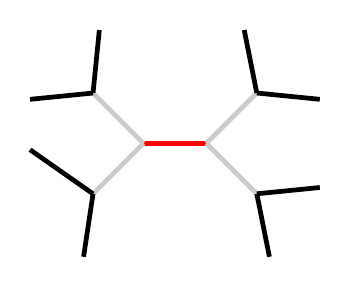
\begin{tikzpicture}[scale=0.8]
    % Boundaries
    \draw[line width=0.6mm, red] (0,0) -- (1,0);
    %
    \draw[line width=0.6mm, black!20] (0,0) -- (-0.8,0.8);
    \draw[line width=0.6mm, black] (-0.8,0.8) -- (-0.7, 1.8);
    \draw[line width=0.6mm, black] (-0.8,0.8) -- (-1.8,0.7);
    %
    \draw[line width=0.6mm, black!20] (0,0) -- (-0.8,-0.8);
    \draw[line width=0.6mm, black] (-0.8,-0.8) -- (-1.8, -0.1);
    \draw[line width=0.6mm, black] (-0.8,-0.8) -- (-0.95, -1.8);
    %
    \draw[line width=0.6mm, black!20] (1,0) -- (1.8,0.8);
    \draw[line width=0.6mm, black] (1.8,0.8) -- (1.6, 1.8);
    \draw[line width=0.6mm, black] (1.8,0.8) -- (2.8,0.7);
    %
    \draw[line width=0.6mm, black!20] (1,0) -- (1.8,-0.8);
    \draw[line width=0.6mm, black] (1.8,-0.8) -- (2, -1.8);
    \draw[line width=0.6mm, black] (1.8,-0.8) -- (2.8,-0.7);
    \end{tikzpicture}
    \label{fig:poll3}
    }\hspace{5em}
    \subfloat[] {    
    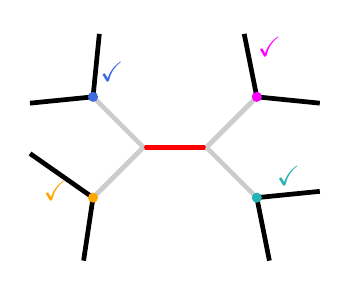
\begin{tikzpicture}[scale=0.8]
    % Boundaries
    \draw[line width=0.6mm, red] (0,0) -- (1,0);
    %
    \draw[line width=0.6mm, black!20] (0,0) -- (-0.8,0.8);
    \draw[line width=0.6mm, black] (-0.8,0.8) -- (-0.7, 1.8);
    \draw[line width=0.6mm, black] (-0.8,0.8) -- (-1.8,0.7);
    %
    \draw[line width=0.6mm, black!20] (0,0) -- (-0.8,-0.8);
    \draw[line width=0.6mm, black] (-0.8,-0.8) -- (-1.8, -0.1);
    \draw[line width=0.6mm, black] (-0.8,-0.8) -- (-0.95, -1.8);
    %
    \draw[line width=0.6mm, black!20] (1,0) -- (1.8,0.8);
    \draw[line width=0.6mm, black] (1.8,0.8) -- (1.6, 1.8);
    \draw[line width=0.6mm, black] (1.8,0.8) -- (2.8,0.7);
    %
    \draw[line width=0.6mm, black!20] (1,0) -- (1.8,-0.8);
    \draw[line width=0.6mm, black] (1.8,-0.8) -- (2, -1.8);
    \draw[line width=0.6mm, black] (1.8,-0.8) -- (2.8,-0.7);
    % Vertices
    %\filldraw [Magenta] (0,0) circle (2pt);
    \filldraw [RoyalBlue] (-0.8,0.8) circle (2pt);
    \filldraw [Orange] (-0.8,-0.8) circle (2pt);
    %\filldraw [Green] (1,0) circle (2pt);
    \filldraw [Fuchsia] (1.8,0.8) circle (2pt);
    \filldraw [TealBlue] (1.8,-0.8) circle (2pt);
    % Votes
    \node[draw=none, color=RoyalBlue] at (-0.5, 1.2) {$\checkmark$};
    \node[draw=none, color=Orange] at (-1.4, -0.7) {$\checkmark$};
    \node[draw=none, color=Fuchsia] at (2, 1.6) {$\checkmark$};
    \node[draw=none, color=TealBlue] at (2.3, -0.45) {$\checkmark$};
    \end{tikzpicture}
    \label{fig:poll4}
    }
    \caption{Polling system scheme.}
    \label{fig:pollingscheme}
\end{figure}
\end{frame}

\begin{frame}{Parallel Management - The Polling System}
    \begin{algorithmic}[1]
\Procedure{Poll}{$\mathcal{S}$}
\State $\boundaries_{\text{flip}} \gets$ Clear boundaries count to 0 and vertices votes
\State $\boundaries_{\text{flip}} \gets$ Vertices votes for their uninhibited boundary with lowest $t_{\text{ext}}$
\State $\boundaries_{\text{flip}} \gets$ Boundaries counts the votes received
\State $\boundaries_{\text{flip}} \gets$ Select uninhibited boundaries with two votes
\State $\boundaries_{\text{flip}} \gets$ Inhibit neighbor boundaries
\State \Return $\mathcal{S}$ \Comment{New inhibited state of boundaries}
\EndProcedure
\end{algorithmic}
\end{frame}

\begin{frame}{Parallel Management - The Polling System}
    \begin{algorithmic}[1]
\Procedure{PollingSystem}{boundaries $\boundaries$}
\State $\boundaries \gets$ Clear flip and inhibited state for each boundary
\State $\boundaries \gets$ Update $t_{\text{ext}}$ for each boundary
\State $\boundaries_{\text{flip}} \gets$ Boundaries to flip with $t_{\text{ext}} \in [0, \Delta t]$
\State $\mathcal{S}_0 \gets$ Initial inhibited state of boundaries
%\State $convergence \gets$ False
\For {$i: 1,\dotsc,n$}
    \State $\mathcal{S}_i \gets \textsc{Poll}(\mathcal{S}_{i-1})$
    \If{$\mathcal{S}_i = \mathcal{S}_{i-1}$}
    \State \Return
    \EndIf
\EndFor
\EndProcedure
\end{algorithmic}
\end{frame}

\section[3D Implicit-transition Model]{More on the Implicit-transition Model for 3D Grain Growth}

\begin{frame}{More on the Implicit-transition Model}
If we choose to move with normal vectors to each boundary instead of tangents, that is:
%
\begin{equation*}
    \dot{\mathbf{P}}^{(\grn)} = \sum_{\bnd^{(k)} \in \grn} \sigma_k \mathbf{N}_k,
\end{equation*}
%
we decrease the energy monotonically.
\begin{figure}
    \centering
    \includegraphics[trim={0 1em 0 3em},clip=true,scale=0.4]{figures/3d_voronoi/3D_energy2.pdf}
\end{figure}
\vspace{-1em}
However we still obtain some unstable behavior, probably related to grains that should have been removed.
\end{frame}
\end{document}


